\documentclass[a4paper,titlepage,11pt,twosides,floatssmall]{mwrep}
\usepackage[left=2.5cm,right=2.5cm,top=2.5cm,bottom=2.5cm]{geometry}
\usepackage[OT1]{fontenc}
\usepackage{polski}
\usepackage{amsmath}
\usepackage{amsfonts}
\usepackage{amssymb}
\usepackage{graphicx}
\usepackage{url}
\usepackage{tikz}
\usetikzlibrary{arrows,calc,decorations.markings,math,arrows.meta}
\usepackage{rotating}
\usepackage[percent]{overpic}
\usepackage[cp1250]{inputenc}
\usepackage{xcolor}
\usepackage{pgfplots}
\usetikzlibrary{pgfplots.groupplots}
\usepackage{listings}
\usepackage{matlab-prettifier}
\usepackage{enumitem,amssymb}
\definecolor{szary}{rgb}{0.95,0.95,0.95}
\usepackage{siunitx}
\sisetup{detect-weight,exponent-product=\cdot,output-decimal-marker={,},per-mode=symbol,binary-units=true,range-phrase={-},range-units=single}
\SendSettingsToPgf
%konfiguracje pakietu listings
\lstset{
	backgroundcolor=\color{szary},
	frame=single,
	breaklines=true,
}
\lstdefinestyle{customlatex}{
	basicstyle=\footnotesize\ttfamily,
	%basicstyle=\small\ttfamily,
}
\lstdefinestyle{customc}{
	breaklines=true,
	frame=tb,
	language=C,
	xleftmargin=0pt,
	showstringspaces=false,
	basicstyle=\small\ttfamily,
	keywordstyle=\bfseries\color{green!40!black},
	commentstyle=\itshape\color{purple!40!black},
	identifierstyle=\color{blue},
	stringstyle=\color{orange},
}
\lstdefinestyle{custommatlab}{
	captionpos=t,
	breaklines=true,
	frame=tb,
	xleftmargin=0pt,
	language=matlab,
	showstringspaces=false,
	%basicstyle=\footnotesize\ttfamily,
	basicstyle=\scriptsize\ttfamily,
	keywordstyle=\bfseries\color{green!40!black},
	commentstyle=\itshape\color{purple!40!black},
	identifierstyle=\color{blue},
	stringstyle=\color{orange},
}

%wymiar tekstu (bez �ywej paginy)
\textwidth 160mm \textheight 247mm

%ustawienia pakietu pgfplots
\pgfplotsset{
tick label style={font=\scriptsize},
label style={font=\small},
legend style={font=\small},
title style={font=\small}
}

\def\figurename{Rys.}
\def\tablename{Tab.}

%konfiguracja liczby p�ywaj�cych element�w
\setcounter{topnumber}{0}%2
\setcounter{bottomnumber}{3}%1
\setcounter{totalnumber}{5}%3
\renewcommand{\textfraction}{0.01}%0.2
\renewcommand{\topfraction}{0.95}%0.7
\renewcommand{\bottomfraction}{0.95}%0.3
\renewcommand{\floatpagefraction}{0.35}%0.5

\begin{document}
\frenchspacing
\pagestyle{uheadings}

%strona tytu�owa
\title{\bf Sprawozdanie z projektu i �wiczenia laboratoryjnego nr 1, zadanie nr 1\vskip 0.1cm}
\author{Imi� i Nazwisko, Imi� i Nazwisko, Imi� i Nazwisko}
\date{2017}

\makeatletter
\renewcommand{\maketitle}{\begin{titlepage}
\begin{center}{\LARGE {\bf
Wydzia� Elektroniki i Technik Informacyjnych}}\\
\vspace{0.4cm}
{\LARGE {\bf Politechnika Warszawska}}\\
\vspace{0.3cm}
\end{center}
\vspace{5cm}
\begin{center}
{\bf \LARGE Projektowanie uk�ad�w sterowania\\ (projekt grupowy) \vskip 0.1cm}
\end{center}
\vspace{1cm}
\begin{center}
{\bf \LARGE \@title}
\end{center}
\vspace{2cm}
\begin{center}
{\bf \Large \@author \par}
\end{center}
\vspace*{\stretch{6}}
\begin{center}
\bf{\large{Warszawa, \@date\vskip 0.1cm}}
\end{center}
\end{titlepage}
}
\makeatother

\maketitle

\tableofcontents
\chapter{Wst�p}
Sprawozdania przygotowywane w~ramach projekt�w i~�wicze� laboratoryjnych musz� by� opracowane w~systemie \LaTeX. System sk�adu dokument�w \LaTeX \ jest ca�kowicie darmowy, ale umo�liwia opracowanie bardzo dobrze z�o�onych dokument�w. Do przygotowania sprawozdania nale�y wykorzysta� klas� \verb+mwrep+ z~pakietu klas \verb+mwcls+ \cite{litWolinski2013} oraz klas� \verb+polski+. W~przypadku d�u�szych opracowa� (ksi��ek, prac dyplomowych) nale�y wykorzysta� klas� \verb+mwbk+.

Je�eli dost�pne s� rysunki w~formacie \verb+pdf+, najwygodniej do przetworzenia dokumentu u�y� polecenia \verb+pdflatex+, kt�re bezpo�rednio generuje dokument w formacie \verb+pdf+. Polecenie \verb+latex+ wymaga rysunk�w w formacie \verb+ps+ lub \verb+eps+ i~generuje dokument w~formacie \verb+dvi+, kt�ry nast�pnie mo�na przekszta�ci� do formatu \verb+eps+ lub \verb+pdf+. Nie u�ywamy rysunk�w zapisanych w~plikach bitmapowych (\verb+bmp+, \verb+jpg+, \verb+png+). Jedynym wyj�tkiem s� zdj�cia.

Istnieje wiele podr�cznik�w do nauki zasad sk�adania dokument�w w~\LaTeX u, np. doskona�a praca zbiorowa \cite{litOetiker2007} lub ew. podr�cznik Wikibooks \cite{litlatexwiki2017}. Do edycji dokument�w mo�na wykorzysta� np. program \TeX nicCenter, dost�pny pod adresem \url{http://www.texniccenter.org}. W~przypadku problem�w warto poszuka� rozwi�zania na forum \url{http://tex.stackexchange.com}.

W~dalszej cz�ci dokumentu podano najwa�niejsze wymagania dotycz�ce wzor�w matematycznych, tabeli i~rysunk�w. Najszybsz� metod� prowadz�c� do otrzymania dokumentu jest modyfikacja niniejszego szablonu.
\chapter{Wzory matematyczne}
Stosujemy przecinek dziesi�tny, a~nie kropk� dziesi�tn�. Aby unikn�� dodatkowego odst�pu, stosujemy zapis \verb+\num{1,2345}+ lub \verb+\num{1.2345}+, co prowadzi do \num{1,2345}, a~nie \verb+$1,2345$+, co prowadzi do $1,2345$. Stosujemy zapis \num{1.2345e10}, a~nie $1{,}2345\times 10^{10}$. Powy�szy zapis mo�na stosowa� r�wnie� w trybie matematycznym, np. \verb+$\num{1.2345e10}$+ skompiluje si� do $\num{1.2345e10}$.

\section{Sta�e i~zmienne, indeksowanie}
Skalarne sta�e i~zmienne zapisujemy w~trybie matematycznym, np. $x$, $y$, $z$. Stosujemy indeksy dolne, np. $x_i$, g�rne, np. $x^j$, lub oba, np. $x_i^j$. Mo�na r�wnie� zastosowa� indeksy w~nawiasach, np. $y(k)$. Je�eli indeks zapisany jest czcionk� pochy��, spodziewamy si�, �e przyjmuje on warto�� liczbow� (liczby naturalne), np. $x_i$ dla $i=1,\ldots,10$. Je�eli natomiast zastosujemy oznaczenie $x_{\mathrm{i}}$, to w�wczas indeks $\mathrm{i}$ nie przyjmuje �adnej warto�ci, jest on integraln� cz�ci� zmiennej lub sta�ej. Dlatego oznaczaj�c horyzont sterowania stosujemy symbol $N_{\mathrm{u}}$, a~nie $N_u$, co by sugerowa�o, �e indeks $u$ przyjmuje pewne warto�ci z zakresu liczb naturalnych. Analogicznie, sta�a czasowa ca�kowania oznaczana jest jako $T_{\mathrm{i}}$, a~nie jako $T_i$, sta�a czasowa r�niczkowania to $T_{\mathrm{d}}$, a nie $T_d$. Sygna� warto�ci zadanej oznaczamy przez $y^{\mathrm{zad}}$, a~nie przez $y^{zad}$.

Nie nale�y stosowa� czcionki pochy�ej r�wnie� do tekst�w, kt�re uzupe�niaj� wyra�enia matematyczne, np. zamiast b��dnej postaci
\begin{equation}
y(x)=
\begin{cases}
x^2 & gdy \ x\le 0\\
x^3 & gdy \ x>0
\end{cases}
\nonumber
\end{equation}
powinno by�
\begin{equation}
y(x)=
\begin{cases}
x^2 & \textrm{gdy } x\le 0\\
x^3 & \textrm{gdy } x>0
\end{cases}
\nonumber
\end{equation}
Odst�py w trybie matematycznym wymuszamy za pomoc� instrukcji \verb+\+, \verb+\quad+, \verb+\qquad+ itd.

\section{Wektory}
Do oznaczenia wektor�w najcz�ciej stosujemy symbole pogrubione, np. $\boldsymbol{x}$, $\triangle\boldsymbol{u}(k)$. Pami�tamy, �e w matematyce wektory zawsze s� pionowe. Wektory, kt�rych elementami s� skalary, zapisujemy wi�c jako
\begin{equation}
\triangle\boldsymbol{u}(k)=\left[\triangle u(k|k) \ \ldots \ \triangle u(k+N_{\mathrm{u}}-1|k) \right]^{\mathrm{T}}
\end{equation}
lub w~postaci
\begin{equation}
\triangle\boldsymbol{u}(k)=\left[
\begin{array}{c}
\triangle u(k|k)\\
\vdots\\
\triangle u(k+N_{\mathrm{u}}-1|k)
\end{array}
\right]
\label{w_dUk}
\end{equation}
Je�eli u�ywamy wektor�w, kt�rych elementami sk�adowymi s� inne wektory, najwygodniej zapisa� je pionowo. Np. elementami wektora (\ref{w_dUk}) s� podwektory
\begin{equation}
\triangle u(k+p|k)=\left[
\begin{array}{c}
\triangle u_1(k+p|k)\\
\vdots\\
\triangle u_{n_{\mathrm{u}}}(k+p|k)
\end{array}
\right]
\label{w_dukp}
\end{equation}
gdzie $p=1,\ldots,N_{\mathrm{u}}$. A wi�c ka�dy z~wektor�w (\ref{w_dukp}) ma d�ugo�� $n_{\mathrm{u}}$, wektor (\ref{w_dUk}) ma d�ugo�� $n_{\mathrm{u}}N_{\mathrm{u}}$.

\section{Macierze}
Do oznaczenia macierzy najcz�ciej stosujemy symbole pogrubione, np. macierz dynamiczna w~algorytmie DMC dla procesu o~jednym wej�ciu i~jednym wyj�ciu ma wymiar $N \times N_{\mathrm{u}}$ i struktur�
\begin{equation}
\boldsymbol{G}=\left[
\begin{array}
{cccc}
s_{1} & 0 & \ldots & 0\\
s_{2} & s_{1} & \ldots & 0\\
\vdots & \vdots & \ddots & \vdots\\
s_{N} & s_{N-1} & \ldots &  s_{N-N_{\mathrm{u}}+1}
\end{array}
\right]
\end{equation}
W~przypadku procesu o~$n_{\mathrm{u}}$ wej�ciach i~$n_{\mathrm{y}}$ wyj�ciach ma ona  wymiar $N\times N_{\mathrm{u}}$ i posta�
\begin{equation}
\boldsymbol{G}=\left[
\begin{array}
{cccc}
\boldsymbol{S}_{1} & \boldsymbol{0}_{n_{\mathrm{y}}\times n_{\mathrm{u}}} & \ldots & \boldsymbol{0}_{n_{\mathrm{y}}\times n_{\mathrm{u}}}\\
\boldsymbol{S}_{2} & \boldsymbol{S}_{1} & \ldots & \boldsymbol{0}_{n_{\mathrm{y}}\times n_{\mathrm{u}}}\\
\vdots & \vdots & \ddots & \vdots\\
\boldsymbol{S}_{N} & \boldsymbol{S}_{N-1} & \ldots &  \boldsymbol{S}_{N-N_{\mathrm{u}}+1}%
\end{array}
\right]
\label{w_G}
\end{equation}
gdzie ka�da z~macierzy sk�adowych ma wymiar $n_{\mathrm{y}}\times n_{\mathrm{u}}$
\begin{equation}
\boldsymbol{S}_p=\left[
\begin{array}
{ccc}
s_p^{1,1} & \ldots & s_p^{1,n_{\mathrm{u}}}\\
\vdots & \ddots & \vdots\\
s_p^{n_{\mathrm{y}},1} & \ldots & s_p^{n_{\mathrm{y}},n_{\mathrm{u}}}
\end{array}
\right]
\end{equation}
gdzie $p=1,\ldots,N$. A~wi�c macierz (\ref{w_G}) ma wymiar $n_{\mathrm{y}}N\times n_{\mathrm{u}}N_{\mathrm{u}}$.

\section{Wi�ksze wyra�enia matematyczne}
W~przypadku d�ugich wzor�w nie nale�y korzysta� z~otoczenia \verb+equation+, poniewa� wz�r taki zwykle nie~mie�ci si� na stronie o przyj�tej szeroko�ci, np.
\begin{equation}
y(k)=b_1u(k-1)+b_2u(k-2)+b_3u(k-3)+b_4u(k-4)+b_5u(k-5)-a_1y(k-1)-a_2y(k-2)-a_3y(k-3)-a_4y(k-4)-a_5y(k-5)
\end{equation}
Nale�y zastosowa� otoczenie \verb+align+, co prowadzi do wzoru
\begin{align}
y(k)&=b_1u(k-1)+b_2u(k-2)+b_3u(k-3)+b_4u(k-4)+b_5u(k-5)\nonumber\\
&\quad -a_1y(k-1)-a_2y(k-2)-a_3y(k-3)-a_4y(k-4)-a_5y(k-5)\label{w_yk}
\end{align}
Nie stosujemy otoczenia \verb+split+ z~powodu b��dnego centrowania. Numer wzoru z�o�onego z~wielu wierszy umieszczamy tylko w~ostatnim wierszu.





\chapter{Tabele}
W~praktyce bardzo cz�sto nale�y wyr�wna� liczby wzgl�dem cyfr znacz�cych w~poszczeg�lnych kolumnach (czyli przecinek dziesi�tny ma by� we wszystkich wierszach tabeli umieszczony w~tym samym miejscu w~pionie). Do wyr�wnania liczb mo�na wykorzysta� pakiet \verb+siunitx+, co zastosowano w tab.~\ref{t_wyrownanie_do_znaku_przecinek3} (pakiety \verb+rccol+ oraz \verb+dcolumn+ maj� mniejsze mo�liwo�ci).

Je�eli tabela jest szersza ni� szeroko�� strony, nale�y zastosowa� otoczenie \verb+sidewaystable+ z~pakietu \verb+rotating+, co wykorzystano w~tab.~\ref{t_wyrownanie_do_znaku_przecinek4}.

W~zamieszczonych tabelkach wykorzystano polecenie \verb+\rule+ do wstawienia linii o~zerowej szeroko�ci do wierszy tabelek, kt�re s� zbyt w�skie.

Je�eli standardowa szeroko�� kolumn jest za ma�a, nale�y w~dowolnym wierszu wstawi� z~obu stron zawarto�ci kom�rki polecenia \verb+\hspace{odleg�o��}+, kt�re zapewniaj� odpowiedni� szeroko��. Modyfikacj� tak� zastosowano w~drugiej kolumnie tab.~\ref{t_wyrownanie_do_znaku_przecinek3}.

%\begin{table}
%[b] \caption{Por�wnanie liczby parametr�w~(LP) i~dok�adno�ci~(SSE) modeli}
%\label{t_wyrownanie_do_znaku_przecinek1}
%\centering
%\begin{small}
%\begin{tabular}{|l|c|r @{$,$} l|r @{$,$} l|r @{$,$} l|}
%\hline
%\multicolumn{1}{|c|}{Model\rule{0pt}{3.5mm}} & LP &
%\multicolumn{2}{c|}{$\mathrm{SSE_{ucz}}$} & \multicolumn{2}{c|}{$\mathrm{SSE_{wer}}$} & \multicolumn{2}{c|}{$\mathrm{SSE_{test}}$}\\\hline
%Liniowy \rule{0pt}{3.5mm}& \phantom{0}4 & $90$&$1815$ & $70$&$7787$ & \multicolumn{2}{c|}{$-$}\\
%Neuronowy, $K=1$ & \phantom{0}7 & $10$&$1649$ & $10$&$3895$ & \multicolumn{2}{c|}{$-$}\\
%Neuronowy, $K=2$ & 13 & $0$&$3282$ & $0$&$3257$ & \multicolumn{2}{c|}{$-$}\\
%Neuronowy, $K=3$ & 19 & $0$&$2014$ & $0$&$1827$ & $0$&$1468$\\
%Neuronowy, $K=4$ & 25 & $0$&$1987$ & $0$&$1906$ & \multicolumn{2}{c|}{$-$}\\
%Neuronowy, $K=5$ & 31 & $0$&$1364$ & $0$&$1971$ & \multicolumn{2}{c|}{$-$}\\
%Neuronowy, $K=6$ & 37 & $0$&$1340$ & $0$&$2044$ & \multicolumn{2}{c|}{$-$}\\
%%Neuronowy, $K=7$ & 43 & $0$&$1280$ & $0$&$2939$ & \multicolumn{2}{c|}{$-$}\\
%\hline
%\end{tabular}
%\end{small}
%\end{table}

\begin{table}
	[b] \caption{Por�wnanie liczby parametr�w~(LP) i~dok�adno�ci~(SSE) modeli}
	\label{t_wyrownanie_do_znaku_przecinek1}
	\centering
	\sisetup{table-format = 2.4}
	\begin{small}
		\begin{tabular}{|l|S[table-format=2]|S|S|S|}
			\hline
			\multicolumn{1}{|c|}{Model\rule{0pt}{3.5mm}} & LP & $\mathrm{SSE_{ucz}}$ & $\mathrm{SSE_{wer}}$ & $\mathrm{SSE_{test}}$ \\ \hline
			Liniowy \rule{0pt}{3.5mm}                    &  4 & 90.1815              & 70.7787              & \textemdash         \\
			Neuronowy, $K=1$                             &  7 & 10.1649              & 10.3895              & \textemdash         \\
			Neuronowy, $K=2$                             & 13 & 0.3282               & 0.3257               & \textemdash         \\
			Neuronowy, $K=3$                             & 19 & 0.2014               & 0.1827               & 0.1468                \\
			Neuronowy, $K=4$                             & 25 & 0.1987               & 0.1906               & \textemdash         \\
			Neuronowy, $K=5$                             & 31 & 0.1364               & 0.1971               & \textemdash         \\
			Neuronowy, $K=6$                             & 37 & 0.1340               & 0.2044               & \textemdash         \\ \hline
		\end{tabular}
	\end{small}
\end{table}

%\begin{table}
%[b] \caption{Por�wnanie liczby parametr�w~(LP) i~dok�adno�ci~(SSE) modeli}
%\label{t_wyrownanie_do_znaku_przecinek2}
%\centering
%\begin{small}
%\begin{tabular}{|l|c|r @{$,$} l|r @{$,$} l|r @{$,$} l|}
%\hline
%\multicolumn{1}{|c|}{Model\rule{0pt}{3.5mm}} & LP &
%\multicolumn{2}{c|}{$\mathrm{SSE_{ucz}}$} & \multicolumn{2}{c|}{$\mathrm{SSE_{wer}}$} & \multicolumn{2}{c|}{$\mathrm{SSE_{test}}$}\\\hline
%Liniowy\rule{0pt}{3.5mm} & \phantom{0}4 & $9$&$1815\cdot10^1$ & $7$&$7787\cdot 10^1$ & \multicolumn{2}{c|}{$-$}\\
%Neuronowy, $K=1$ & \phantom{0}7 & $1$&$1649\cdot 10^1$ & $1$&$3895\cdot 10^1$ & \multicolumn{2}{c|}{$-$}\\
%Neuronowy, $K=2$ & 13 & $3$&$2821\cdot 10^{-1}$ & $3$&$2568\cdot 10^{-1}$ & \multicolumn{2}{c|}{$-$}\\
%Neuronowy, $K=3$ & 19 & $2$&$0137\cdot 10^{-1}$ & $1$&$8273\cdot 10^{-1}$ & $1$&$4682\cdot 10^{-1}$\\
%Neuronowy, $K=4$ & 25 & $1$&$9868\cdot 10^{-1}$ & $1$&$9063\cdot 10^{-1}$ & \multicolumn{2}{c|}{$-$}\\
%Neuronowy, $K=5$ & 31 & $1$&$3642\cdot 10^{-1}$ & $1$&$9712\cdot 10^{-1}$ & \multicolumn{2}{c|}{$-$}\\
%Neuronowy, $K=6$ & 37 & $1$&$3404\cdot 10^{-1}$ & $2$&$0440\cdot 10^{-1}$ & \multicolumn{2}{c|}{$-$}\\
%%Neuronowy, $K=7$ & 43 & $1$&$2801\cdot 10^{-1}$ & $2$&$9391\cdot 10^{-1}$ & \multicolumn{2}{c|}{$-$}\\
%\hline
%\end{tabular}
%\end{small}
%\end{table}

\begin{table}
	[b] \caption{Por�wnanie liczby parametr�w~(LP) i~dok�adno�ci~(SSE) modeli}
	\label{t_wyrownanie_do_znaku_przecinek2}
	\centering
	\sisetup{table-format = 1.4e-1}
	\begin{small}
		\begin{tabular}{|l|S[table-format=2]|S|S|S|}
			\hline
			\multicolumn{1}{|c|}{Model\rule{0pt}{3.5mm}} & LP & $\mathrm{SSE_{ucz}}$ & $\mathrm{SSE_{wer}}$ & $\mathrm{SSE_{test}}$ \\ \hline
			Liniowy\rule{0pt}{3.5mm} &  4 & 9.1815e1  & 7.7787e1  & \textemdash\\
			Neuronowy, $K=1$         &  7 & 1.1649e1  & 1.3895e1  & \textemdash\\
			Neuronowy, $K=2$         & 13 & 3.2821e-1 & 3.2568e-1 & \textemdash\\
			Neuronowy, $K=3$         & 19 & 2.0137e-1 & 1.8273e-1 & 1.4682e-1\\
			Neuronowy, $K=4$         & 25 & 1.9868e-1 & 1.9063e-1 & \textemdash\\
			Neuronowy, $K=5$         & 31 & 1.3642e-1 & 1.9712e-1 & \textemdash\\
			Neuronowy, $K=6$         & 37 & 1.3404e-1 & 2.0440e-1 & \textemdash\\ \hline
		\end{tabular}
	\end{small}
\end{table}

%\begin{table}
%[b] \caption{Por�wnanie z�o�ono�ci obliczeniowej}
%\label{t_wyrownanie_do_znaku_przecinek3}
%\centering
%\begin{small}
%\begin{tabular}{|l|c|R{1}{2}|R{1}{2}|R{2}{2}|R{2}{2}|R{2}{2}|R{3}{2}|}
%	\hline
%	\multicolumn{1}{|c|}{Algorytm\rule{0pt}{3.25mm}} & \hspace{0.5cm} $N$ \hspace{0.5cm} & \multicolumn{1}{c|}{$N_{\mathrm{u}}=1$} & \multicolumn{1}{c|}{$N_{\mathrm{u}}=2$} & \multicolumn{1}{c|}{$N_{\mathrm{u}}=3$} & \multicolumn{1}{c|}{$N_{\mathrm{u}}=4$} & \multicolumn{1}{c|}{$N_{\mathrm{u}}=5$} & \multicolumn{1}{c|}{$N_{\mathrm{u}}=10$}\tabularnewline
%\hline
%NPL\rule{0pt}{3.5mm} & \phantom{0}5 & 0,3954 & 0,5326 & 0,8482 & 1,2868 & 1,9179 & \multicolumn{1}{c|}{$-$}\tabularnewline
%NO & \phantom{0}5 & 2,6129 & 5,0372 & 8,0029 & 12,6476 & 18,3668 & \multicolumn{1}{c|}{$-$}\tabularnewline
%NO$_{\mathrm{apr}}$\rule[-1.5mm]{0pt}{3.5mm} & \phantom{0}5 & 2,4654 & 4,3206 & 7,9801 & 15,2479 & 26,5298 & \multicolumn{1}{c|}{$-$}\tabularnewline
%\hline
%NPL\rule{0pt}{3.5mm} & 10 & 0,6274 & 0, 7874 & 1,1366 & 1,6201 & 2,3101 & 9,1346\tabularnewline
%NO & 10 & 5,2040 & 9,0378 & 13,5571 & 19,1675 & 26,2604 & 76,5018\tabularnewline
%NO$_{\mathrm{apr}}$\rule[-1.5mm]{0pt}{3.5mm} & 10 & 4,3828 & 7,5813 & 12,6279 & 20,0911 & 31, 7747 & 154,1544\tabularnewline
%\hline
%\end{tabular}
%\end{small}
%\end{table}

\begin{table}
	[b] \caption{Por�wnanie z�o�ono�ci obliczeniowej}
	\label{t_wyrownanie_do_znaku_przecinek3}
	\centering
	\sisetup{table-auto-round=true}
	\begin{small}
		\begin{tabular}{|l|S[table-format=2]|S[table-format=1.2]|S[table-format=1.2]|S[table-format=2.2]|S[table-format=2.2]|S[table-format=2.2]|S[table-format=3.2]|}
			\hline
			\multicolumn{1}{|c|}{Algorytm\rule{0pt}{3.25mm}} & \hspace{0.5cm} $N$ \hspace{0.5cm} & ${N_{\mathrm{u}}=1}$ & ${N_{\mathrm{u}}=2}$ & ${N_{\mathrm{u}}=3}$ & ${N_{\mathrm{u}}=4}$ & ${N_{\mathrm{u}}=5}$ & ${N_{\mathrm{u}}=10}$ \\ \hline
			NPL\rule{0pt}{3.5mm} & 5 & 0,3954 & 0,5326 & 0,8482 & 1,2868 & 1,9179 & \textemdash \\
			NO & 5 & 2,6129 & 5,0372 & 8,0029 & 12,6476 & 18,3668 & \textemdash \\
			NO$_{\mathrm{apr}}$\rule[-1.5mm]{0pt}{3.5mm} & \phantom{0}5 & 2,4654 & 4,3206 & 7,9801 & 15,2479 & 26,5298 & \textemdash \\ \hline
			NPL\rule{0pt}{3.5mm} & 10 & 0,6274 & 0, 7874 & 1,1366 & 1,6201 & 2,3101 & 9,1346 \\
			NO & 10 & 5,2040 & 9,0378 & 13,5571 & 19,1675 & 26,2604 & 76,5018 \\		
			NO$_{\mathrm{apr}}$\rule[-1.5mm]{0pt}{3.5mm} & 10 & 4,3828 & 7,5813 & 12,6279 & 20,0911 & 31, 7747 & 154,1544 \\ \hline
		\end{tabular}
	\end{small}
\end{table}

%\begin{sidewaystable}
%[b] \caption{Por�wnanie z�o�ono�ci obliczeniowej}
%\label{t_wyrownanie_do_znaku_przecinek4}
%\centering
%\begin{small}
%\begin{tabular}{|l|c|R{1}{2}|R{1}{2}|R{2}{2}|R{2}{2}|R{2}{2}|R{3}{2}|R{3}{2}|R{3}{2}|R{3}{2}|}
%\hline
%\multicolumn{1}{|c|}{Algorytm\rule{0pt}{3.25mm}} & $N$ & \multicolumn{1}{c|}{$N_{\mathrm{u}}=1$} & \multicolumn{1}{c|}{$N_{\mathrm{u}}=2$} &
%\multicolumn{1}{c|}{$N_{\mathrm{u}}=3$} &
%\multicolumn{1}{c|}{$N_{\mathrm{u}}=4$} &
%\multicolumn{1}{c|}{$N_{\mathrm{u}}=5$} &
%\multicolumn{1}{c|}{$N_{\mathrm{u}}=10$} &
%\multicolumn{1}{c|}{$N_{\mathrm{u}}=15$} &
%\multicolumn{1}{c|}{$N_{\mathrm{u}}=20$} &
%\multicolumn{1}{c|}{$N_{\mathrm{u}}=30$}\tabularnewline
%\hline
%NPL\rule{0pt}{3.5mm} & \phantom{0}5 & 0,3954 & 0,5326 & 0,8482 & 1,2868 & 1,9179 & \multicolumn{1}{c|}{$-$} & \multicolumn{1}{c|}{$-$} & \multicolumn{1}{c|}{$-$} & \multicolumn{1}{c|}{$-$}\tabularnewline
%NO & \phantom{0}5 & 2,6129 & 5,0372 & 8,0029 & 12,6476 & 18,3668 & \multicolumn{1}{c|}{$-$} & \multicolumn{1}{c|}{$-$} & \multicolumn{1}{c|}{$-$} & \multicolumn{1}{c|}{$-$}\tabularnewline
%NO$_{\mathrm{apr}}$\rule[-1.5mm]{0pt}{3.5mm} & \phantom{0}5 & 2,4654 &  4,3206 & 7,9801 & 15,2479 & 26,5298 & \multicolumn{1}{c|}{$-$} & \multicolumn{1}{c|}{$-$} & \multicolumn{1}{c|}{$-$} & \multicolumn{1}{c|}{$-$}\tabularnewline
%\hline
%\end{tabular}
%\end{small}
%\end{sidewaystable}

\begin{sidewaystable}
	[b] \caption{Por�wnanie z�o�ono�ci obliczeniowej}
	\label{t_wyrownanie_do_znaku_przecinek4}
	\centering
	\centering
	\sisetup{table-auto-round=true}
	\begin{small}
		\begin{tabular}{|l|S[table-format=2]|S[table-format=1.2]|S[table-format=1.2]|S[table-format=2.2]|S[table-format=2.2]|S[table-format=2.2]|S[table-format=3.2]|S[table-format=3.2]|S[table-format=3.2]|S[table-format=3.2]|}
			\hline
			\multicolumn{1}{|c|}{Algorytm\rule{0pt}{3.25mm}} & $N$ & ${N_{\mathrm{u}}=1}$ & ${N_{\mathrm{u}}=2}$ &
			${N_{\mathrm{u}}=3}$ &
			${N_{\mathrm{u}}=4}$ &
			${N_{\mathrm{u}}=5}$ &
			${N_{\mathrm{u}}=10}$ &
			${N_{\mathrm{u}}=15}$ &
			${N_{\mathrm{u}}=20}$ &
			${N_{\mathrm{u}}=30}$\\
			\hline
			NPL\rule{0pt}{3.5mm} & \phantom{0}5 & 0,3954 & 0,5326 & 0,8482 & 1,2868 & 1,9179 & \textemdash & \textemdash & \textemdash & \textemdash\\
			NO & \phantom{0}5 & 2,6129 & 5,0372 & 8,0029 & 12,6476 & 18,3668 & \textemdash & \textemdash & \textemdash & \textemdash\\
			NO$_{\mathrm{apr}}$\rule[-1.5mm]{0pt}{3.5mm} & \phantom{0}5 & 2,4654 &  4,3206 & 7,9801 & 15,2479 & 26,5298 & \textemdash & \textemdash & \textemdash & \textemdash\\
			\hline
		\end{tabular}
	\end{small}
\end{sidewaystable}
\chapter{Rysunki}
Wszystkie elementy dokumentu opracowanego w~systemie \LaTeX powinny wygl�da� jednolicie. Do wykonywania rysunk�w korzystamy wi�c z mechanizm�w oferowanych przez dodatkowe pakiety \LaTeX a, nie do��czamy rysunk�w wykonanych jako�ciowo r�nych, np. wykonanych w~programie Word. Nie u�ywamy rysunkach zapisanych w~plikach bitmapowych, lecz w~plikach wektorowych (\verb+pdf+, ew. \verb+ps+ lub \verb+eps+). Jedynym wyj�tkiem s� zdj�cia.

\section{Schematy blokowe}
Do opracowania schemat�w blokowych najlepiej wykorzysta� j�zyk opisu rysunk�w \verb+TikZ/PGF+ \cite{litTantau2015}. Przy wykonywaniu prostych rysunk�w po prostu opisujemy je za pomoc� polece� dodaj�cych kolejne elementy, tzn. prostok�ty, okr�gi, linie. Na przyk�ad, ci�g polece�:
\begin{lstlisting}[style=customlatex,frame=single] 
\begin{figure}[b]
\centering
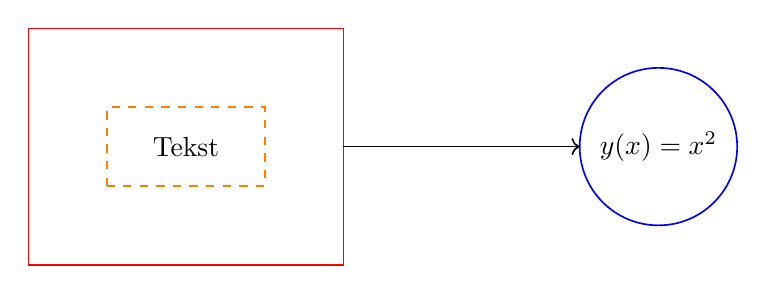
\begin{tikzpicture}
\draw [red, semithick] (0,0) rectangle (4,3);
\draw [orange, semithick,dashed] (1,1) rectangle (3,2);
\draw [->,semithick] (4,1.5) -- (7,1.5);
\draw [blue, semithick] (8,1.5) circle [radius=1];
\node at (2,1.5) {Tekst};
\node at (8,1.5) {$y(x)=x^2$};
\end{tikzpicture}
\end{figure}
\end{lstlisting}
pozwala narysowa� figury geometryczne przedstawione na rys. \ref{r_tikz_przyklad}. Zwr��my uwag�, �e napis oraz wz�r s� z�o�one aktualnie wykorzystywan� czcionk�, jej wielko�� jest taka sama jak w~ca�ym dokumencie.

\begin{figure}[b]
\centering
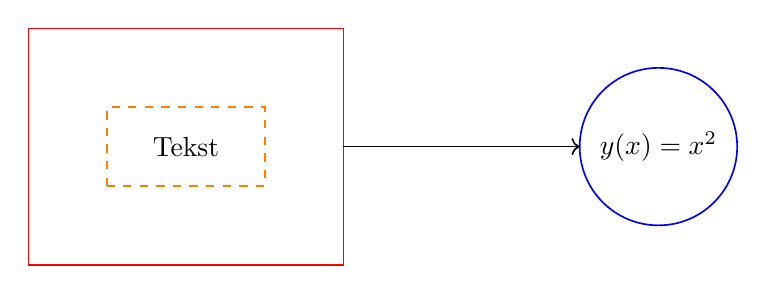
\begin{tikzpicture}
\draw [red, semithick] (0,0) rectangle (4,3);
\draw [orange, semithick,dashed] (1,1) rectangle (3,2);
\draw [->,semithick] (4,1.5) -- (7,1.5);
\draw [blue, semithick] (8,1.5) circle [radius=1];;
\node at (2,1.5) {Tekst};
\node at (8,1.5) {$y(x)=x^2$};
\end{tikzpicture}
%\caption{Przyk�adowy rysunek wykorzystany w~j�zyku \verb+TikZ/PGF+}
\caption{Tekst Przyk�adowy rysunek wykorzystany w~j�zyku \texttt{TikZ/PGF}}
\label{r_tikz_przyklad}
\end{figure}

Przy wi�kszych rysunkach mo�na wykorzysta� programy umo�liwiaj�ce ich przygotowanie przy wykorzystaniu �rodowiska graficznego, np. \verb+TikzEdt+ (\url{http://www.tikzedt.org/}), \verb+TpX+ (\url{http://tpx.sourceforge.net/}), \verb+ktikz+ (\url{https://www.linux-apps.com/p/1126914/}), \verb+GraTeX+ (\url{https://sourceforge.net/projects/gratex/}).

Mo�na r�wnie� wykorzysta� starsze, klasyczne pakiety \verb+picture+, \verb+epic+, \verb+eepic+. R�wnie� w~tych przypadkach mo�na ,,r�cznie'' opisywa� poszczeg�lne elementy graficzne lub skorzysta� ze �rodowiska graficznego, np. \verb+LaTeXPiX+ (\url{http://latexpix.software.informer.com/}), kt�re znacznie przyspiesza prac�. Inne narz�dzia, umo�liwiaj�ce opracowanie rysunk�w wysokiej jako�ci, to \verb+METAPOST+ oraz \verb+PSTricks+.

\section{Funkcje statyczne}
Do wykonywania wykres�w prezentuj�cych wyniki symulacji i~eksperyment�w stosuje si� pakiet \verb+PGFPLOTS+ \cite{litFeuersanger2016}. Za��my, �e w~katalogu \verb+rysunki/dane_stat+ znajduje si� plik \verb+dane_fx.txt+ zawieraj�cy w~pierwszej kolumnie warto�ci argumentu $x$, natomiast w~drugiej kolumnie warto�ci funkcji $f(x)$
\begin{lstlisting}[style=customlatex,frame=single]
  -10.0000 -808.7350
   -9.0000 -696.4791
   -8.0000 -539.7850
   -7.0000 -386.1268
   -6.0000 -291.5881
   -5.0000 -267.6436
   -4.0000 -268.9551
   -3.0000 -233.3995
   -2.0000 -137.5303
   -1.0000  -16.4788
         0   70.0000
    1.0000   94.1212
    2.0000   87.2697
    3.0000  112.8005
    4.0000  209.4449
    5.0000  357.3564
    6.0000  498.0119
    7.0000  589.6732
    8.0000  647.4150
    9.0000  730.9209
   10.0000  891.2650
\end{lstlisting}
oraz podobny plik \verb+dane_gx.txt+, definiuj�cy funkcj� $g(x)$. Aby narysowa� te funkcje stosuje si� polecenia:
\begin{lstlisting}[style=customlatex,frame=single]
\begin{figure}[t]
\centering
\begin{tikzpicture}
\begin{axis}[
width=0.5\textwidth,
xmin=-10,xmax=10,ymin=-1000,ymax=1000,
xlabel={$x$},
ylabel={$f(x), \ g(x)$},
xtick={-10,-5,0,5,10},
ytick={-1000,-500,0,500,1000},
legend pos=south east,
y tick label style={/pgf/number format/1000 sep=},
]
\addplot[red, semithick]                file {rysunki/dane_stat/dane_fx.txt};
\addplot[blue,semithick,densely dashed] file {rysunki/dane_stat/dane_gx.txt};
\legend{$f(x)$,$g(x)$}
\end{axis}
\end{tikzpicture}
\caption{Przyk�adowy rysunek funkcji $f(x)$ i~$g(x)$ wykonany 
w~j�zyku \texttt{PGFPLOTS}}
\label{r_pgfplots_funkcje}
\end{figure}
\end{lstlisting}
Otrzymany rezultat przedstawiono na rys.~\ref{r_pgfplots_funkcje}. Istnieje mo�liwo�� ustawienia wielko�ci czcionek liczb umieszczonych: na osiach (\verb+tick label style+), w~oznaczeniach osi (\verb+label style+), w~legendzie (\verb+legend style+) oraz w~tytule rysunku (\verb+title style+). Przyk�adowa konfiguracja zmieniaj�ca wielko�� czcionek jest nast�puj�ca:
\begin{lstlisting}[style=customlatex,frame=single]
\pgfplotsset{
tick label style={font=\tiny},
label style={font=\footnotesize},
legend style={font=\footnotesize},
title style={font=\footnotesize}
}
\end{lstlisting}

\begin{figure}[tb]
\centering
\begin{tikzpicture}
\begin{axis}[
width=0.5\textwidth,
xmin=-10,xmax=10,ymin=-1000,ymax=1000,
xlabel={$x$},
ylabel={$f(x), \ g(x)$},
xtick={-10,-5,0,5,10},
ytick={-1000,-500,0,500,1000},
legend pos=south east,
y tick label style={/pgf/number format/1000 sep=},
]
\addplot[red, semithick]                file {rysunki/dane_stat/dane_fx.txt};
\addplot[blue,semithick,densely dashed] file {rysunki/dane_stat/dane_gx.txt};
\legend{$f(x)$,$g(x)$}
\end{axis}
\end{tikzpicture}
\caption{Przyk�adowy rysunek funkcji $f(x)$ i~$g(x)$ wykonany w~j�zyku \texttt{PGFPLOTS} (rysunek jest kompilowany przy ka�dym przetworzenia pliku �r�d�owego}
\label{r_pgfplots_funkcje}
\end{figure}

Opisany spos�b implementacji rysunk�w jest poprawny, ale ma powa�n� wad�, poniewa� \LaTeX{}   potrzebuje do�� du�o czasu na ich przetworzenie. Okazuje si� to du�ym mankamentem szczeg�lnie w�wczas, gdy w~dokumencie znajduje si� du�o skomplikowanych rysunk�w. Skutecznym rozwi�zaniem jest przygotowanie rysunk�w i~zapis ich do plik�w \verb+pdf+, a~nast�pnie do��czenie ich do g��wnego dokumentu poleceniem \verb+\includegraphics+. Plik \verb+zapisz_pdf_funkcje.tex+, umo�liwiaj�cy zapisanie rysunku do pliku \verb+funkcje.pdf+, znajduje si� w~katalogu \verb+rysunki/zapisz_pdf+ i~ma nast�puj�c� posta�:
\lstinputlisting[style=customlatex,frame=single]{rysunki/zapisz_pdf/zapisz_pdf_funkcje.tex}

Polecenie
\begin{lstlisting}[style=customlatex,frame=single]
pdflatex -shell-escape zapisz_pdf_funkcje.tex
\end{lstlisting}
zapisuje plik \verb+funkcje.pdf+. Umieszczaj�c wiele definicji rysunk�w w~jednym pliku �r�d�owym mo�na  generowa� wiele rysunk�w w~postaci plik�w \verb+pdf+.

Przy du�ych zbiorach danych \LaTeX{} zg�asza b��d pami�ci. Nale�y w�wczas zastosowa� \hbox{Lua\LaTeX}. Rysunek do��cza si� do dokumentu ci�giem instrukcji:
\begin{lstlisting}[style=customlatex,frame=single]
\begin{figure}[tb]
\centering
\includegraphics[scale=1]{pgfplots_pdf/funkcje}
\caption{Przyk�adowy rysunek funkcji $f(x)$ i~$g(x)$ wykonany
w~j�zyku \texttt{PGFPLOTS}}
\label{r_pgfplots_funkcje}
\end{figure}
\end{lstlisting}
Otrzymany rezultat przedstawiono na rys.~\ref{r_pgfplots_funkcje_pdf}. Oczywi�cie, rysunki \ref{r_pgfplots_funkcje} i~\ref{r_pgfplots_funkcje_pdf} s� bardzo podobne, jedyn� r�nic� jest wielko�� czcionek.

Nie nale�y skalowa� rysunku, gdy� zmieni to wielko�� zastosowanej czcionki. Je�eli zachodzi konieczno�� zmiany wielko�ci rysunku, nale�y zmodyfikowa� plik �r�d�owy generuj�cy rysunek.

Je�eli rysunek jest szerszy ni� szeroko�� strony, nale�y zastosowa� otoczenie \verb+sidewaysfigure+ z~pakietu \verb+rotating+, kt�re dzia�a analogicznie jak otoczenie \verb+sidewaystable+.

W~bardzo podobny spos�b przygotowuje si� rysunki tr�jwymiarowe \cite{litFeuersanger2016}.

\begin{figure}[ptb]
\centering
\includegraphics[scale=1]{rysunki/zapisz_pdf/funkcje}
\caption{Przyk�adowy rysunek funkcji $f(x)$ i~$g(x)$ wykonany
w~j�zyku \texttt{PGFPLOTS} i~zapisany w~pliku \texttt{funkcje.pdf}}
\label{r_pgfplots_funkcje_pdf}
\end{figure}

\section{Wyniki symulacji i~eksperyment�w}
Za��my, �e w~katalogu \verb+rysunki/symulacje11+ znajduje si� plik \verb+yzad.txt+ zawieraj�cy w~pierwszej kolumnie pomiary czasu $t$ (w~sekundach), natomiast w~drugiej kolumnie pr�bki sygna�u warto�ci zadanej $y^{\mathrm{zad}}$. Wykonano symulacje algorytmu regulacji GPC przy pi�ciu r�nych warto�ciach parametru $\lambda$: $\num{0,1}$, $\num{0,2}$, $\num{0,5}$, $\num{1}$ i~$\num{2}$. Przebiegi sygna�u steruj�cego $u$ zapisano w~plikach \verb+u_lambda_0_1.txt+, \verb+u_lambda_0_2.txt+, \verb+u_lambda_0_5.txt+, \verb+u_lambda_1.txt+ i~\verb+u_lambda_2.txt+, natomiast przebiegi sygna�u wyj�ciowego procesu $y$ zapisano w~plikach \verb+y_lambda_0_1.txt+, \verb+y_lambda_0_2.txt+, \verb+y_lambda_0_5.txt+, \verb+y_lambda_1.txt+ i~\verb+y_lambda_2.txt+. Przygotowano plik \verb+zapisz_pdf_symulacje11.tex+, umo�liwiaj�cy zapisanie rysunku do pliku \verb+symulacje11.pdf+. Znajduje si� on w~katalogu \verb+rysunki/zapisz_pdf+ i~ma nast�puj�c� posta�:

\lstinputlisting[style=customlatex,frame=single]{rysunki/zapisz_pdf/zapisz_pdf_symulacje11.tex}
Polecenie
\begin{lstlisting}[style=customlatex,frame=single]
pdflatex -shell-escape zapisz_pdf_symulacje11.tex
\end{lstlisting}
zapisuje plik \verb+symulacje11.pdf+. Rysunek do��cza si� do dokumentu instrukcj� \verb+\includegraphics+. Efekt przedstawiono na rys.~\ref{r_pgfplots_symulacje11_pdf}. Zwr��my uwag�, �e do narysowania wynik�w symulacji dla kolejnych warto�ci parametru $\lambda$ zastosowano r�ne kolory oraz r�ne style linii (linia ci�g�a, linia przerywana, itd.). Umo�liwia to �atwe rozr�nienie dokument�w na czarno-bia�ym wydruku. Przy wydruku kolorowym oraz dokumentach elektronicznych mo�na zrezygnowa� ze stosowania r�nych styl�w linii, do ich rozr�nienia wystarczaj�ce s� kolory, pod warunkiem jednak, �e kolejne krzywe nie s� po�o�one bardzo blisko siebie.

Pakiet \verb+PGFPLOTS+ mo�na skonfigurowa� w~taki spos�b, aby na osiach stosowane by�y liczby z~przecinkiem dziesi�tnym w~miejsce kropki dziesi�tnej \cite{litFeuersanger2016}.

Czasami ze wzgl�du na ograniczon� obj�to�� dokumentu nale�y zmniejszy� rysunki. Aby zmniejszy� obj�to�� mo�na zastosowa� u�o�enie poziome dw�ch rysunk�w, prezentuj�cych wyniki symulacji procesu. Przygotowano plik \verb+zapisz_pdf_symulacje11_wersja2.tex+, umo�liwiaj�cy zapisanie rysunku do pliku \verb+symulacje11_wersja2.pdf+. Znajduje si� on w~katalogu \verb+rysunki/zapisz_pdf+ i~ma nast�puj�c� posta�:
\lstinputlisting[style=customlatex,frame=single]{rysunki/zapisz_pdf/zapisz_pdf_symulacje11_wersja2.tex}
Rysunek do��cza si� do dokumentu instrukcj� \verb+\includegraphics+. Efekt przedstawiono na rys.~\ref{r_pgfplots_symulacje11_wersja2_pdf}.

\begin{figure}[tb]
\centering
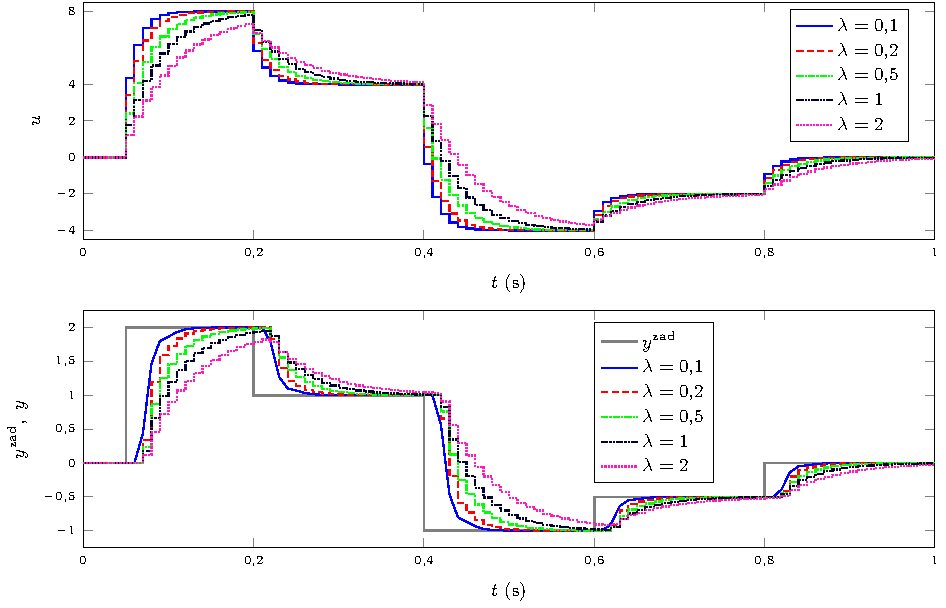
\includegraphics[scale=1]{rysunki/zapisz_pdf/symulacje11}
%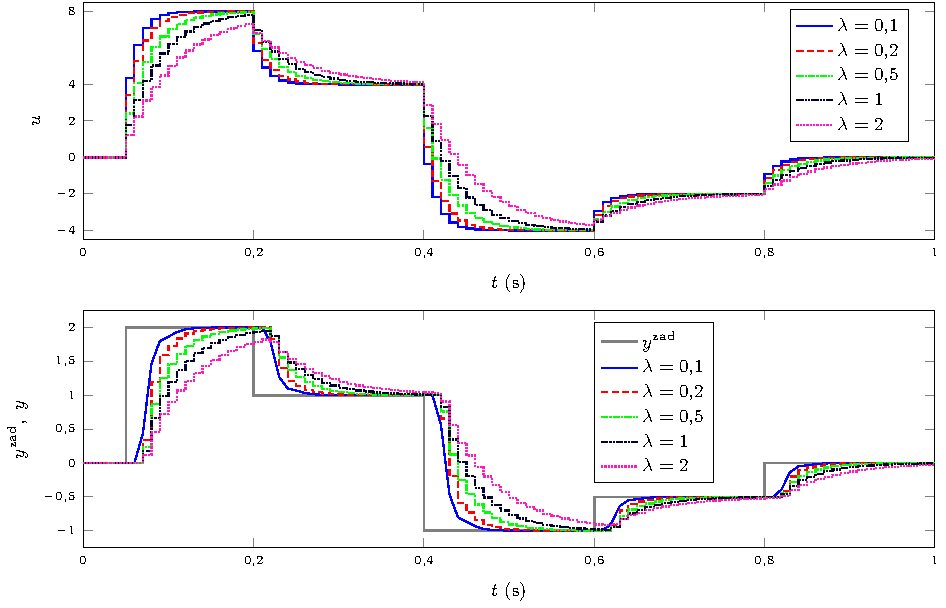
\includegraphics[scale=1]{rysunki/zapisz_pdf/symulacje11}
\caption{Przyk�adowy rysunek wynik�w symulacji procesu jednowymiarowego wykonany
w~j�zyku \texttt{PGFPLOTS} i~zapisany w~pliku \texttt{symulacje11.pdf}}
\label{r_pgfplots_symulacje11_pdf}
\end{figure}

\begin{figure}[tb]
\centering
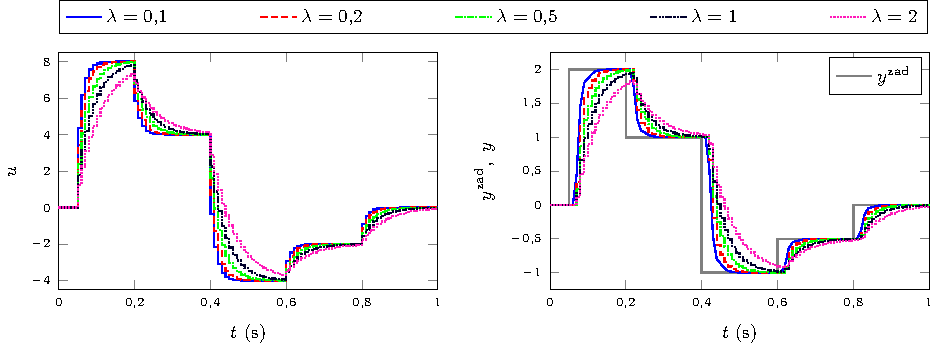
\includegraphics[scale=1]{rysunki/zapisz_pdf/symulacje11_wersja2}
\caption{Przyk�adowy rysunek wynik�w symulacji procesu jednowymiarowego wykonany
w~j�zyku \texttt{PGFPLOTS} i~zapisany w~pliku \texttt{symulacje11\_wersja2.pdf}}
\label{r_pgfplots_symulacje11_wersja2_pdf}
\end{figure}

Za��my, �e w~katalogu \verb+rysunki/symulacje22+ znajduj� si� wyniki symulacji procesu o~dw�ch wej�ciach i~dw�ch wyj�ciach zapisane w~plikach: \verb+yzad1.txt+, \verb+yzad2.txt+, \verb+u1.txt+, \verb+u2.txt+, \verb+y1.txt+, \verb+y2.txt+. W~pierwszej kolumnie tych plik�w podano czas $t$ (w~sekundach), natomiast w~drugiej kolumnie warto�� odpowiedniej zmiennej. Plik \verb+zapisz_pdf_symulacje22.tex+, umo�liwiaj�cy zapisanie rysunku do pliku \verb+symulacje22.pdf+ znajduje si� w~katalogu \verb+rysunki/zapisz_pdf+ i~ma nast�puj�c� posta�:
\lstinputlisting[style=customlatex,frame=single]{rysunki/zapisz_pdf/zapisz_pdf_symulacje22.tex}
Rysunek do��cza si� do dokumentu instrukcj� \verb+\includegraphics+. Efekt przedstawiono na rys.~\ref{r_pgfplots_symulacje22_pdf}.

Aby zmniejszy� obj�to�� mo�na nieco inaczej u�o�y� 4 rysunki, prezentuj�ce wyniki symulacji procesu dwuwymiarowego. Przygotowano plik \verb+zapisz_pdf_symulacje22_wersja2.tex+, umo�liwiaj�cy zapisanie rysunku do pliku \verb+symulacje22_wersja2.pdf+. Znajduje si� on w~katalogu \verb+rysunki/zapisz_pdf+ i~ma nast�puj�c� posta�:
\lstinputlisting[style=customlatex,frame=single]{rysunki/zapisz_pdf/zapisz_pdf_symulacje22_wersja2.tex}
Rysunek do��cza si� do dokumentu instrukcj� \verb+\includegraphics+. Efekt przedstawiono na rys.~\ref{r_pgfplots_symulacje22_wersja2_pdf}.

\begin{figure}[p]
\centering
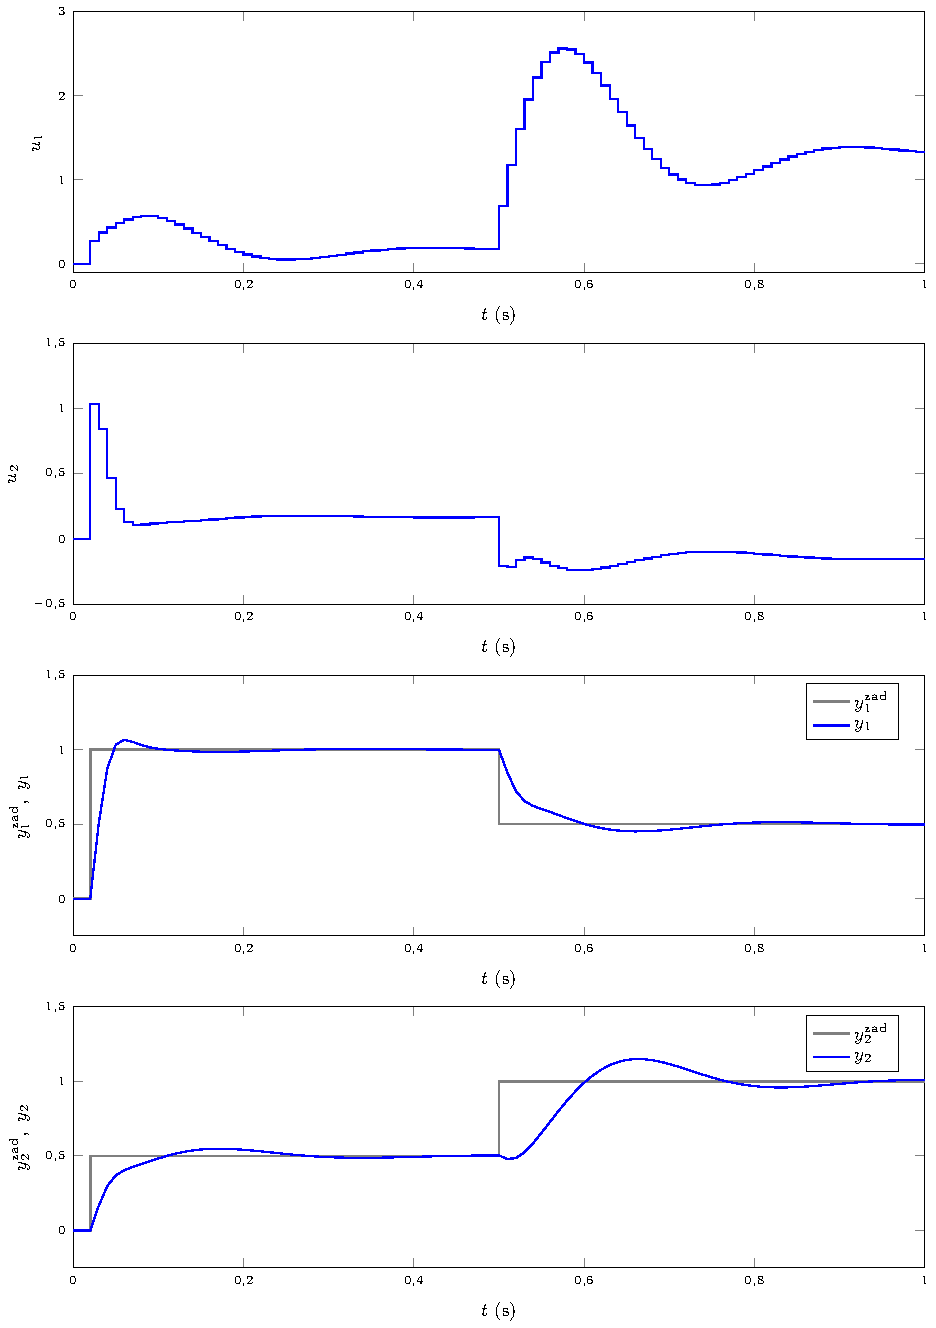
\includegraphics[scale=1]{rysunki/zapisz_pdf/symulacje22}
\caption{Przyk�adowy rysunek wynik�w symulacji procesu dwuwymiarowego wykonany
w~j�zyku \texttt{PGFPLOTS} i~zapisany w~pliku \texttt{symulacje22.pdf}}
\label{r_pgfplots_symulacje22_pdf}
\end{figure}

\begin{figure}[b]
\centering
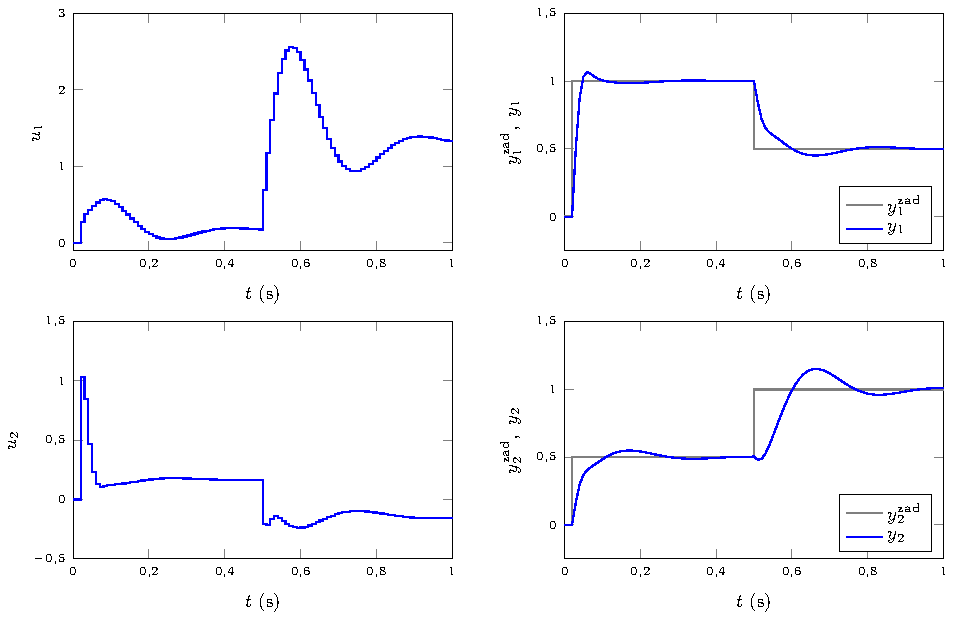
\includegraphics[scale=1]{rysunki/zapisz_pdf/symulacje22_wersja2}
\caption{Przyk�adowy rysunek wynik�w symulacji procesu dwuwymiarowego wykonany
w~j�zyku \texttt{PGFPLOTS} i~zapisany w~pliku \texttt{symulacje22\_wersja2.pdf}}
\label{r_pgfplots_symulacje22_wersja2_pdf}
\end{figure}

\section{Kolory}
Przy umieszczaniu kilku wykres�w na tym samym rysunku nale�y zastosowa� kolory r�ni�ce si� od siebie w~znacznym stopniu, nie mo�na stosowa� kolor�w podobnych, np. kilku odcieni tego samego koloru. Do generacji palety kolor�w spe�niaj�cej takie wymagania mo�na u�y� funkcji \verb+distinguishable_colors.m+, udost�pnionej na stronie \url{https://www.mathworks.com/matlabcentral/}. Zestaw dwudziestu kolor�w zosta� przedstawiony na rys.~\ref{r_zestaw_kolorow}. Ich definicja w~palecie RGB jest nast�puj�ca:
\begin{lstlisting}[style=customlatex,frame=single]
         0         0    1.0000
    1.0000         0         0
         0    1.0000         0
         0         0    0.1724
    1.0000    0.1034    0.7241
    1.0000    0.8276         0
         0    0.3448         0
    0.5172    0.5172    1.0000
    0.6207    0.3103    0.2759
         0    1.0000    0.7586
         0    0.5172    0.5862
         0         0    0.4828
    0.5862    0.8276    0.3103
    0.9655    0.6207    0.8621
    0.8276    0.0690    1.0000
    0.4828    0.1034    0.4138
    0.9655    0.0690    0.3793
    1.0000    0.7586    0.5172
    0.1379    0.1379    0.0345
    0.5517    0.6552    0.4828
\end{lstlisting}
\definecolor{kolor5}{rgb}{1.0000,0.1034,0.7241}
Opr�cz kolor�w standardowych oraz dodatkowych, kt�re s� zdefiniowane w~pakiecie \verb+xcolor+, w�asne kolory definiujemy poleceniem \verb+\definecolor+. Na przyk�ad, pi�ty kolor z~zestawu definiujemy poleceniem \verb+\definecolor{kolor5}{rgb}{1.0000,0.1034,0.7241}+, {\color{kolor5}co umo�liwia osi�gni�cie nast�puj�cego efektu}.

\begin{figure}[b]
\centering

\includegraphics[width=0.75\textwidth,height=0.1\textheight]{rysunki/kolory}
\caption{Paleta 20 kolor�w}
\label{r_zestaw_kolorow}
\end{figure}

\section{Lokalizacja rysunk�w (i~tabel)}
Wszystkie rysunki i~tabele umieszczamy jako ,,p�ywaj�ce", a~wi�c w otoczeniu \verb+figure+ oraz \verb+table+ nie stosujemy opcji \verb+[h]+ i~\verb+[H]+. Aby unikn�� umieszczenia rysunk�w w~tek�cie kolejnego rozdzia�u nale�y zastosowa� polecenie \verb+\FloatBarrier+ z~pakietu \verb+placeins+.



\chapter{Listingi program�w}
Do zamieszczenia program�w mo�na zastosowa� otoczenie \verb+verbatim+, ale znacznie wi�ksze mo�liwo�ci oferuje pakiet \verb+listings+. Przyk�adowy program w~j�zyku C ma posta�:
\begin{lstlisting}[style=customc,frame=single] 
//Hello World in C
#include <stdio.h>
int main (void)
{
   puts ("Hello World!");
   return 0;
}
\end{lstlisting}
natomiast przyk�adowy program w~j�zyku \verb+Matlab+ jest nast�puj�cy:
%\begin{lstlisting}[style=custommatlab,frame=single]
\begin{lstlisting}[style=Matlab-editor]
%Hello World in Matlab
clear all;

disp('Hello World!');
\end{lstlisting} 







\begin{thebibliography}{99}
\bibitem{litFeuersanger2016}
C. Feuers\"anger: Manual for package PGFPLOTS. \url{ftp://ftp.gust.org.pl/TeX/graphics/pgf/contrib/pgfplots/doc/pgfplots.pdf}, 2016.

\bibitem{litOetiker2007}
T. Oetiker, H. Partl, I. Hyna, E. Schlegl: Nie za kr�tkie wprowadzenie do systemu \LaTeXe. \url{ftp://ftp.gust.org.pl/pub/CTAN/info/lshort/polish/lshort2e.pdf}, 2007.

\bibitem{litTantau2015}
T. Tantau: The TikZ and PGF Packages Manual for version 3.0.1a. \url{ftp://ftp.gust.org.pl/TeX/graphics/pgf/base/doc/pgfmanual.pdf}, 2015.

\bibitem{litWolinski2013}
M. Woli�ski: Moje W�asne CLaSy dokument�w dla \LaTeX a 2e \url{http://marcinwolinski.pl/mwcls.html}, 2013.

\bibitem{litlatexwiki2017}
Wikibooks: \LaTeX. \url{https://en.wikibooks.org/wiki/LaTeX}, 2017.

\end{thebibliography}
\appendix
\newlength\fwidth
\newlength\fheight

\chapter{Uwagi do wykonywania sprawozda�}
\section{Kodowanie znak�w}
Aktualnie kodowanie znak�w ustawione jest na cp1250 (czasem oznaczane jako windows-1250). Wiele program�w dokonuje automatycznej analizy dokumentu otwieranego i na podstawie jego zawarto�ci odgaduje jakie kodowanie powinno zosta� zastosowane dla danego pliku. O ile przyk�adowo TeXstudio (dobre IDE na pocz�tek) nie ma problem�w z automatycznym okre�leniem kodowania dla pliku \verb|sprawozdanie_szablon.tex|, poniewa� rozpoznaje np. zawart� w nim linijk� \verb|\usepackage[cp1250]{inputenc}|, o tyle pozosta�e pliki tej linijki nie zawieraj�, co powoduje cz�sto b��dnie odgadni�te kodowanie. Aby wskaza� dla danego pliku jakie kodowanie ma zosta� u�yte, mo�na wstawi� na poczatku tego pliku linijk� o tre�ci \newline\verb|% !TEX encoding = cp1250|\newline kt�ra spowoduje wymuszenie u�ycia tego w�a�nie kodowania w tym pliku.

Oczywi�cie ewentualne przej�cie na kodowanie UTF-8 wymaga� b�dzie:
\begin{itemize}
	\item zmiany linijki \verb|\usepackage[cp1250]{inputenc}| na \verb|\usepackage[utf8]{inputenc}|,
	\item zmiany kodowania w poszczeg�lnych plikach z kodowania cp1250 na UTF-8,
	\item ewentualn� zmian� linijek \verb|% !TEX encoding = cp1250| na \verb|% !TEX encoding = utf8|.
\end{itemize}
Warto na koniec przekompilowa� wszelkie pliki, aby nie by�o problem�w ze sp�jno�ci�, a wi�c w szczeg�lno�ci wyrzuci� wszystki pliki o rozszerzeniu \verb|.aux| i \verb|.pdf|.

\section{Nie nale�y u�ywa� zwrot�w w cudzys�owiu i narzeka�}
Potrzeba u�ycia wyra�enia otoczonego znakami ,, oraz '' (prosz� nie stosowa� ameryka�skiej formy cudzys�owiu!) sugeruje, �e pisz�cy nie zna poprawnego okre�lenia opisywanego zjawiska. W takim wypadku nale�y zg��bi� k�opotliwy temat lub w szczeg�lno�ci poprosi� o pomoc prowadz�cego.

R�wnie� nale�y unika� zrzucania winy za niewykonanie zada� na:
\begin{itemize}
	\item ograniczony czas trwania laboratorium,
	\item b��dy we w�asnym kodzie, kt�rych znalezienie trwa�o zbyt d�ugo,
	\item zbyt du�� liczb� zada� do wykonania,
	\item niedzia�aj�cy sprz�t,
	\item zaskakuj�ce dzia�anie programu, kt�rego nikt si� nie spodziewa�,
	\item itp.
\end{itemize} 

Je�li maj� Pa�stwo jakie� problemy z oprogramowaniem/sprz�tem, to nale�y to zg�osi� prowadz�cemu laboratorium. Nie mniej sprz�t jest testowany przed zaj�ciami -- w tym aspekcie problem�w by� nie powinno. 

Odwiedzanie prowadz�cego w ramach konsultacji jest wysoce wskazane i zalecane. Warto korzysta� tak�e z kontaktu mailowego -- wiele prostych problem�w mo�na rozwi�za� t� drog�.

\section{Przecinki zamiast kropek i jednostki}
Stosowanie j�zyka polskiego wymusza na autorze sprawozdania przestrzeganie podstawowych zasad. Jedn� z cz�sto ignorowanych regu� jest stosowanie przecinka zamiast kropki do oddzielenia cz�ci ca�kowitej liczby rzeczywistej od jej cz�ci u�amkowej. Ma to du�y wp�yw na estetyk� sprawozdania.
\begin{center}
\begin{tabular}{llc}
	zapis w \LaTeX & efekt & czy poprawne? \\ \hline
	\verb+$12.345$+ & $12.345$ & nie \\
	\verb+$12,345$+ & $12,345$ & nie \\
	\verb+$\num{12.345}$+ & $\num{12.345}$ & \textbf{tak} \\
	\verb+$\num{12,345}$+ & $\num{12,345}$ & \textbf{tak} \\
\end{tabular}
\end{center}

Ciekawe efekty pojawiaj� si� przy wymienianiu r�nych warto�ci parametr�w w jednym zdaniu, np. 
\newline\noindent,,Do testowania zastosowane zosta�y okresy pr�bkowania $0,01$, $0,1$, $1$, $10$ oraz $100$ sekund.''

Przy okazji warto zwr�ci� uwag� na zapis jednostek:

\begin{center}
\begin{tabular}{llc}
	zapis w \LaTeX & efekt & czy poprawne? \\ \hline
	\verb+$\num{12.345}\mu s$+ & $\num{12.345}\mu s$ & nie \\
	\verb+$\SI{12.345}{\micro s}$+ & $\SI{12.345}{\micro s}$ & \textbf{tak} \\
	\verb+$\num{12.345}\ \mu s$+ & $\num{12.345}\ \mu s$ & nie \\
\end{tabular}
\end{center}

Nawyk pisania kropek zamiast przecink�w w liczbach rzeczywistych cz�sto wywodzi si� ze stylu narzuconego przez j�zyk programowania i dlatego mo�na go zachowa� tylko w listingach -- w sprawozdaniu i na wykresie koniecznie nale�y stosowa� przecinki.

\section{Prosty eksport wykres�w: \texttt{matlab2tikz}}
Poprzez wywo�anie skryptu:
\lstinputlisting[style=Matlab-editor]{./skrypty/wykresy_z_matlaba.m}

a nast�pnie u�ycie w \LaTeX-u polecenia \lstinline[language=tex]|% This file was created by matlab2tikz.
%
\definecolor{mycolor1}{rgb}{0.00000,0.44700,0.74100}%
%
\begin{tikzpicture}

\begin{axis}[%
width=4.521in,
height=3.566in,
at={(0.758in,0.481in)},
scale only axis,
xmin=0,
xmax=3.141,
xlabel style={font=\color{white!15!black}},
xlabel={o� X},
ymin=-1,
ymax=1,
ylabel style={font=\color{white!15!black}},
ylabel={o� Y},
axis background/.style={fill=white}
]
\addplot [color=mycolor1, forget plot]
  table[row sep=crcr]{%
0	0\\
0.001	2e-12\\
0.002	3.2e-11\\
0.003	1.62e-10\\
0.004	5.12e-10\\
0.005	1.25e-09\\
0.006	2.592e-09\\
0.007	4.802e-09\\
0.008	8.192e-09\\
0.009	1.3122e-08\\
0.01	2e-08\\
0.011	2.9282e-08\\
0.012	4.1472e-08\\
0.013	5.7122e-08\\
0.014	7.68319999999999e-08\\
0.015	1.0125e-07\\
0.016	1.31072e-07\\
0.017	1.67041999999999e-07\\
0.018	2.09951999999999e-07\\
0.019	2.60641999999997e-07\\
0.02	3.19999999999995e-07\\
0.021	3.8896199999999e-07\\
0.022	4.68511999999983e-07\\
0.023	5.59681999999971e-07\\
0.024	6.63551999999951e-07\\
0.025	7.81249999999921e-07\\
0.026	9.13951999999873e-07\\
0.027	1.0628819999998e-06\\
0.028	1.22931199999969e-06\\
0.029	1.41456199999953e-06\\
0.03	1.61999999999929e-06\\
0.031	1.84704199999895e-06\\
0.032	2.09715199999846e-06\\
0.033	2.37184199999778e-06\\
0.034	2.67267199999682e-06\\
0.035	3.0012499999955e-06\\
0.036	3.35923199999368e-06\\
0.037	3.74832199999122e-06\\
0.038	4.17027199998791e-06\\
0.039	4.62688199998349e-06\\
0.04	5.11999999997763e-06\\
0.041	5.65152199996992e-06\\
0.042	6.22339199995983e-06\\
0.043	6.83760199994672e-06\\
0.044	7.49619199992979e-06\\
0.045	8.20124999990806e-06\\
0.046	8.95491199988032e-06\\
0.047	9.75936199984508e-06\\
0.048	1.06168319998006e-05\\
0.049	1.15296019997446e-05\\
0.05	1.24999999996745e-05\\
0.051	1.35304019995872e-05\\
0.052	1.46232319994788e-05\\
0.053	1.5780961999345e-05\\
0.054	1.70061119991803e-05\\
0.055	1.83012499989784e-05\\
0.056	1.96689919987318e-05\\
0.057	2.11120019984317e-05\\
0.058	2.26329919980677e-05\\
0.059	2.42347219976277e-05\\
0.06	2.59199999970976e-05\\
0.061	2.76916819964609e-05\\
0.062	2.95526719956983e-05\\
0.063	3.15059219947878e-05\\
0.064	3.35544319937035e-05\\
0.065	3.5701249992416e-05\\
0.066	3.79494719908911e-05\\
0.067	4.03022419890897e-05\\
0.068	4.2762751986967e-05\\
0.069	4.53342419844716e-05\\
0.07	4.8019999981545e-05\\
0.071	5.08233619781204e-05\\
0.072	5.37477119741221e-05\\
0.073	5.67964819694639e-05\\
0.074	5.99731519640483e-05\\
0.075	6.32812499577649e-05\\
0.076	6.6724351950489e-05\\
0.077	7.03060819420801e-05\\
0.078	7.40301119323802e-05\\
0.079	7.79001619212113e-05\\
0.08	8.1919999908374e-05\\
0.081	8.60934418936448e-05\\
0.082	9.04243518767733e-05\\
0.083	9.491664185748e-05\\
0.084	9.9574271835453e-05\\
0.085	0.000104401249810344\\
0.086	0.000109401631781767\\
0.087	0.000114579521749291\\
0.088	0.000119939071712438\\
0.089	0.000125484481670679\\
0.09	0.000131219999623427\\
0.091	0.000137149921570033\\
0.092	0.000143278591509778\\
0.093	0.000149610401441872\\
0.094	0.00015614979136544\\
0.095	0.00016290124927952\\
0.096	0.000169869311183054\\
0.097	0.000177058561074877\\
0.098	0.000184473630953711\\
0.099	0.000192119200818154\\
0.1	0.000199999998666667\\
0.101	0.000208120800497567\\
0.102	0.000216486430309011\\
0.103	0.000225101760098986\\
0.104	0.00023397170986529\\
0.105	0.000243101247605525\\
0.106	0.000252495389317071\\
0.107	0.000262159198997078\\
0.108	0.00027209778864244\\
0.109	0.00028231631824978\\
0.11	0.000292819995815429\\
0.111	0.000303614077335399\\
0.112	0.000314703866805365\\
0.113	0.000326094716220636\\
0.114	0.000337792025576127\\
0.115	0.000349801242866333\\
0.116	0.000362127864085297\\
0.117	0.000374777433226577\\
0.118	0.00038775554228321\\
0.119	0.000401067831247678\\
0.12	0.000414719988111866\\
0.121	0.000428717748867023\\
0.122	0.000443066897503716\\
0.123	0.000457773266011782\\
0.124	0.000472842734380282\\
0.125	0.000488281230597447\\
0.126	0.00050409473065062\\
0.127	0.000520289258526201\\
0.128	0.000536870886209583\\
0.129	0.000553845733685086\\
0.13	0.000571219968935887\\
0.131	0.00058899980794395\\
0.132	0.000607191514689944\\
0.133	0.000625801401153164\\
0.134	0.000644835827311446\\
0.135	0.00066430120114107\\
0.136	0.000684203978616674\\
0.137	0.000704550663711144\\
0.138	0.000725347808395512\\
0.139	0.000746602012638843\\
0.14	0.000768319924408119\\
0.141	0.000790508239668112\\
0.142	0.000813173702381256\\
0.143	0.000836323104507509\\
0.144	0.000859963286004208\\
0.145	0.000884101134825921\\
0.146	0.000908743586924287\\
0.147	0.000933897626247844\\
0.148	0.000959570284741863\\
0.149	0.000985768642348157\\
0.15	0.00101249982700489\\
0.151	0.00103977101464638\\
0.152	0.00106758942920289\\
0.153	0.00109596234260038\\
0.154	0.0011248970747603\\
0.155	0.00115440099359937\\
0.156	0.00118448151502926\\
0.157	0.00121514610295639\\
0.158	0.00124640226928159\\
0.159	0.00127825757389986\\
0.16	0.00131071962470006\\
0.161	0.00134379607756456\\
0.162	0.00137749463636891\\
0.163	0.00141182305298153\\
0.164	0.00144678912726332\\
0.165	0.00148240070706727\\
0.166	0.00151866568823811\\
0.167	0.00155559201461181\\
0.168	0.00159318767801526\\
0.169	0.00163146071826574\\
0.17	0.00167041922317046\\
0.171	0.00171007132852611\\
0.172	0.00175042521811833\\
0.173	0.00179148912372115\\
0.174	0.00183327132509648\\
0.175	0.00187578014999352\\
0.176	0.00191902397414814\\
0.177	0.0019630112212823\\
0.178	0.00200775036310335\\
0.179	0.00205324991930337\\
0.18	0.0020995184575585\\
0.181	0.00214656459352815\\
0.182	0.0021943969908543\\
0.183	0.00224302436116064\\
0.184	0.00229245546405183\\
0.185	0.00234269910711257\\
0.186	0.00239376414590674\\
0.187	0.00244565948397651\\
0.188	0.00249839407284133\\
0.189	0.00255197691199696\\
0.19	0.00260641704891444\\
0.191	0.00266172357903902\\
0.192	0.00271790564578901\\
0.193	0.00277497244055471\\
0.194	0.00283293320269711\\
0.195	0.00289179721954672\\
0.196	0.00295157382640227\\
0.197	0.00301227240652934\\
0.198	0.00307390239115904\\
0.199	0.00313647325948651\\
0.2	0.00319999453866946\\
0.201	0.00326447580382667\\
0.202	0.00332992667803632\\
0.203	0.00339635683233439\\
0.204	0.00346377598571297\\
0.205	0.00353219390511842\\
0.206	0.00360162040544959\\
0.207	0.00367206534955594\\
0.208	0.00374353864823551\\
0.209	0.00381605026023294\\
0.21	0.0038896101922374\\
0.211	0.00396422849888034\\
0.212	0.0040399152827333\\
0.213	0.00411668069430558\\
0.214	0.00419453493204182\\
0.215	0.00427348824231956\\
0.216	0.00435355091944663\\
0.217	0.00443473330565855\\
0.218	0.00451704579111574\\
0.219	0.00460049881390075\\
0.22	0.0046851028600153\\
0.221	0.0047708684633773\\
0.222	0.00485780620581768\\
0.223	0.00494592671707728\\
0.224	0.00503524067480342\\
0.225	0.00512575880454656\\
0.226	0.00521749187975673\\
0.227	0.00531045072177991\\
0.228	0.00540464619985424\\
0.229	0.00550008923110619\\
0.23	0.00559679078054652\\
0.231	0.00569476186106618\\
0.232	0.00579401353343207\\
0.233	0.00589455690628261\\
0.234	0.00599640313612328\\
0.235	0.00609956342732195\\
0.236	0.00620404903210408\\
0.237	0.00630987125054774\\
0.238	0.00641704143057859\\
0.239	0.0065255709679646\\
0.24	0.00663547130631062\\
0.241	0.00674675393705287\\
0.242	0.00685943039945317\\
0.243	0.00697351228059307\\
0.244	0.00708901121536776\\
0.245	0.00720593888647983\\
0.246	0.00732430702443283\\
0.247	0.00744412740752466\\
0.248	0.00756541186184074\\
0.249	0.00768817226124705\\
0.25	0.00781242052738283\\
0.251	0.00793816862965327\\
0.252	0.0080654285852218\\
0.253	0.0081942124590023\\
0.254	0.00832453236365099\\
0.255	0.00845640045955818\\
0.256	0.00858982895483971\\
0.257	0.00872483010532821\\
0.258	0.00886141621456407\\
0.259	0.00899959963378621\\
0.26	0.00913939276192254\\
0.261	0.0092808080455802\\
0.262	0.00942385797903552\\
0.263	0.00956855510422371\\
0.264	0.00971491201072822\\
0.265	0.00986294133576994\\
0.266	0.0100126557641959\\
0.267	0.010164068028468\\
0.268	0.0103171909086509\\
0.269	0.0104720372324002\\
0.27	0.01062861987495\\
0.271	0.0107869517591001\\
0.272	0.0109470458552027\\
0.273	0.0111089151811493\\
0.274	0.0112725728023569\\
0.275	0.0114380318317536\\
0.276	0.0116053054297642\\
0.277	0.0117744068042955\\
0.278	0.0119453492107209\\
0.279	0.0121181459518647\\
0.28	0.0122928103779861\\
0.281	0.0124693558867626\\
0.282	0.0126477959232734\\
0.283	0.0128281439799819\\
0.284	0.0130104135967178\\
0.285	0.0131946183606594\\
0.286	0.0133807719063144\\
0.287	0.0135688879155009\\
0.288	0.0137589801173282\\
0.289	0.0139510622881763\\
0.29	0.0141451482516756\\
0.291	0.0143412518786853\\
0.292	0.0145393870872728\\
0.293	0.0147395678426904\\
0.294	0.0149418081573536\\
0.295	0.0151461220908174\\
0.296	0.0153525237497526\\
0.297	0.0155610272879214\\
0.298	0.0157716469061529\\
0.299	0.0159843968523168\\
0.3	0.016199291421298\\
0.301	0.0164163449549695\\
0.302	0.016635571842165\\
0.303	0.0168569865186509\\
0.304	0.0170806034670978\\
0.305	0.0173064372170508\\
0.306	0.0175345023448996\\
0.307	0.0177648134738481\\
0.308	0.0179973852738821\\
0.309	0.018232232461738\\
0.31	0.0184693698008692\\
0.311	0.018708812101413\\
0.312	0.0189505742201554\\
0.313	0.0191946710604966\\
0.314	0.0194411175724146\\
0.315	0.019689928752428\\
0.316	0.0199411196435591\\
0.317	0.0201947053352945\\
0.318	0.0204507009635464\\
0.319	0.0207091217106115\\
0.32	0.0209699828051309\\
0.321	0.0212332995220467\\
0.322	0.0214990871825599\\
0.323	0.0217673611540862\\
0.324	0.0220381368502108\\
0.325	0.0223114297306423\\
0.326	0.0225872553011664\\
0.327	0.0228656291135973\\
0.328	0.0231465667657287\\
0.329	0.0234300839012842\\
0.33	0.0237161962098655\\
0.331	0.0240049194269004\\
0.332	0.0242962693335895\\
0.333	0.0245902617568515\\
0.334	0.0248869125692673\\
0.335	0.0251862376890236\\
0.336	0.0254882530798541\\
0.337	0.025792974750981\\
0.338	0.0261004187570534\\
0.339	0.0264106011980864\\
0.34	0.0267235382193973\\
0.341	0.0270392460115412\\
0.342	0.0273577408102455\\
0.343	0.0276790388963422\\
0.344	0.0280031565956998\\
0.345	0.0283301102791529\\
0.346	0.028659916362431\\
0.347	0.0289925913060853\\
0.348	0.0293281516154147\\
0.349	0.0296666138403894\\
0.35	0.0300079945755738\\
0.351	0.0303523104600472\\
0.352	0.0306995781773232\\
0.353	0.0310498144552675\\
0.354	0.0314030360660139\\
0.355	0.0317592598258788\\
0.356	0.0321185025952735\\
0.357	0.0324807812786157\\
0.358	0.032846112824238\\
0.359	0.0332145142242958\\
0.36	0.0335860025146725\\
0.361	0.0339605947748833\\
0.362	0.0343383081279769\\
0.363	0.0347191597404353\\
0.364	0.0351031668220718\\
0.365	0.0354903466259267\\
0.366	0.0358807164481612\\
0.367	0.0362742936279496\\
0.368	0.0366710955473681\\
0.369	0.0370711396312835\\
0.37	0.0374744433472378\\
0.371	0.0378810242053317\\
0.372	0.0382908997581055\\
0.373	0.0387040876004181\\
0.374	0.0391206053693231\\
0.375	0.039540470743943\\
0.376	0.0399637014453409\\
0.377	0.0403903152363897\\
0.378	0.0408203299216389\\
0.379	0.0412537633471791\\
0.38	0.0416906334005037\\
0.381	0.0421309580103677\\
0.382	0.042574755146645\\
0.383	0.0430220428201818\\
0.384	0.0434728390826478\\
0.385	0.0439271620263849\\
0.386	0.0443850297842529\\
0.387	0.0448464605294721\\
0.388	0.0453114724754634\\
0.389	0.0457800838756853\\
0.39	0.0462523130234681\\
0.391	0.0467281782518449\\
0.392	0.0472076979333795\\
0.393	0.0476908904799913\\
0.394	0.0481777743427773\\
0.395	0.0486683680118303\\
0.396	0.0491626900160545\\
0.397	0.0496607589229772\\
0.398	0.0501625933385575\\
0.399	0.0506682119069916\\
0.4	0.0511776333105147\\
0.401	0.0516908762691989\\
0.402	0.0522079595407483\\
0.403	0.0527289019202897\\
0.404	0.0532537222401603\\
0.405	0.0537824393696914\\
0.406	0.0543150722149882\\
0.407	0.0548516397187058\\
0.408	0.0553921608598218\\
0.409	0.055936654653404\\
0.41	0.0564851401503751\\
0.411	0.0570376364372725\\
0.412	0.0575941626360049\\
0.413	0.0581547379036033\\
0.414	0.0587193814319697\\
0.415	0.0592881124476193\\
0.416	0.0598609502114204\\
0.417	0.0604379140183283\\
0.418	0.0610190231971154\\
0.419	0.061604297110097\\
0.42	0.0621937551528516\\
0.421	0.0627874167539374\\
0.422	0.0633853013746035\\
0.423	0.0639874285084965\\
0.424	0.064593817681362\\
0.425	0.0652044884507415\\
0.426	0.0658194604056638\\
0.427	0.0664387531663317\\
0.428	0.067062386383803\\
0.429	0.067690379739667\\
0.43	0.0683227529457151\\
0.431	0.0689595257436061\\
0.432	0.069600717904526\\
0.433	0.0702463492288426\\
0.434	0.0708964395457539\\
0.435	0.0715510087129313\\
0.436	0.0722100766161566\\
0.437	0.0728736631689536\\
0.438	0.0735417883122132\\
0.439	0.074214472013813\\
0.44	0.0748917342682305\\
0.441	0.0755735950961501\\
0.442	0.0762600745440638\\
0.443	0.0769511926838659\\
0.444	0.0776469696124407\\
0.445	0.0783474254512441\\
0.446	0.0790525803458785\\
0.447	0.0797624544656606\\
0.448	0.080477068003183\\
0.449	0.0811964411738686\\
0.45	0.0819205942155179\\
0.451	0.0826495473878495\\
0.452	0.0833833209720333\\
0.453	0.0841219352702161\\
0.454	0.0848654106050408\\
0.455	0.0856137673191571\\
0.456	0.086367025774725\\
0.457	0.0871252063529112\\
0.458	0.0878883294533765\\
0.459	0.088656415493757\\
0.46	0.0894294849091359\\
0.461	0.090207558151508\\
0.462	0.0909906556892357\\
0.463	0.0917787980064971\\
0.464	0.0925720056027257\\
0.465	0.0933702989920407\\
0.466	0.0941736987026704\\
0.467	0.0949822252763652\\
0.468	0.0957958992678033\\
0.469	0.0966147412439859\\
0.47	0.097438771783625\\
0.471	0.098268011476521\\
0.472	0.0991024809229309\\
0.473	0.0999422007329285\\
0.474	0.100787191525753\\
0.475	0.101637473929151\\
0.476	0.102493068578704\\
0.477	0.103353996117152\\
0.478	0.104220277193702\\
0.479	0.105091932463331\\
0.48	0.105968982586072\\
0.481	0.106851448226299\\
0.482	0.107739350051994\\
0.483	0.108632708734005\\
0.484	0.109531544945296\\
0.485	0.110435879360184\\
0.486	0.111345732653564\\
0.487	0.112261125500125\\
0.488	0.113182078573557\\
0.489	0.114108612545738\\
0.49	0.11504074808592\\
0.491	0.115978505859893\\
0.492	0.116921906529151\\
0.493	0.11787097075003\\
0.494	0.118825719172843\\
0.495	0.119786172441005\\
0.496	0.12075235119014\\
0.497	0.121724276047176\\
0.498	0.122701967629431\\
0.499	0.123685446543683\\
0.5	0.124674733385228\\
0.501	0.125669848736926\\
0.502	0.126670813168232\\
0.503	0.127677647234214\\
0.504	0.12869037147456\\
0.505	0.129709006412566\\
0.506	0.130733572554114\\
0.507	0.131764090386637\\
0.508	0.132800580378066\\
0.509	0.133843062975765\\
0.51	0.134891558605453\\
0.511	0.135946087670106\\
0.512	0.137006670548851\\
0.513	0.138073327595838\\
0.514	0.139146079139104\\
0.515	0.140224945479416\\
0.516	0.141309946889101\\
0.517	0.142401103610859\\
0.518	0.143498435856562\\
0.519	0.144601963806035\\
0.52	0.145711707605824\\
0.521	0.146827687367943\\
0.522	0.147949923168605\\
0.523	0.149078435046944\\
0.524	0.150213243003706\\
0.525	0.15135436699994\\
0.526	0.152501826955653\\
0.527	0.153655642748466\\
0.528	0.154815834212236\\
0.529	0.155982421135674\\
0.53	0.157155423260933\\
0.531	0.158334860282187\\
0.532	0.159520751844186\\
0.533	0.160713117540794\\
0.534	0.161911976913511\\
0.535	0.163117349449969\\
0.536	0.164329254582416\\
0.537	0.165547711686179\\
0.538	0.166772740078101\\
0.539	0.168004359014968\\
0.54	0.169242587691909\\
0.541	0.170487445240777\\
0.542	0.171738950728513\\
0.543	0.172997123155484\\
0.544	0.174261981453805\\
0.545	0.175533544485636\\
0.546	0.176811831041462\\
0.547	0.178096859838345\\
0.548	0.179388649518162\\
0.549	0.180687218645814\\
0.55	0.18199258570742\\
0.551	0.18330476910848\\
0.552	0.184623787172024\\
0.553	0.185949658136732\\
0.554	0.187282400155034\\
0.555	0.188622031291186\\
0.556	0.18996856951932\\
0.557	0.191322032721476\\
0.558	0.192682438685605\\
0.559	0.19404980510355\\
0.56	0.195424149569\\
0.561	0.196805489575423\\
0.562	0.198193842513972\\
0.563	0.199589225671365\\
0.564	0.200991656227745\\
0.565	0.202401151254503\\
0.566	0.203817727712088\\
0.567	0.205241402447784\\
0.568	0.20667219219346\\
0.569	0.208110113563295\\
0.57	0.209555183051481\\
0.571	0.211007417029887\\
0.572	0.212466831745709\\
0.573	0.213933443319082\\
0.574	0.21540726774067\\
0.575	0.216888320869229\\
0.576	0.218376618429132\\
0.577	0.21987217600788\\
0.578	0.221375009053571\\
0.579	0.222885132872346\\
0.58	0.22440256262581\\
0.581	0.225927313328408\\
0.582	0.227459399844793\\
0.583	0.228998836887141\\
0.584	0.230545639012458\\
0.585	0.232099820619832\\
0.586	0.23366139594768\\
0.587	0.23523037907094\\
0.588	0.236806783898249\\
0.589	0.23839062416908\\
0.59	0.239981913450847\\
0.591	0.241580665135986\\
0.592	0.24318689243899\\
0.593	0.244800608393425\\
0.594	0.246421825848903\\
0.595	0.248050557468026\\
0.596	0.249686815723293\\
0.597	0.25133061289398\\
0.598	0.252981961062976\\
0.599	0.254640872113595\\
0.6	0.256307357726341\\
0.601	0.25798142937565\\
0.602	0.259663098326591\\
0.603	0.261352375631527\\
0.604	0.263049272126752\\
0.605	0.264753798429077\\
0.606	0.266465964932393\\
0.607	0.268185781804186\\
0.608	0.269913258982026\\
0.609	0.271648406170008\\
0.61	0.273391232835162\\
0.611	0.275141748203825\\
0.612	0.27689996125797\\
0.613	0.278665880731502\\
0.614	0.28043951510651\\
0.615	0.282220872609488\\
0.616	0.284009961207507\\
0.617	0.285806788604352\\
0.618	0.287611362236622\\
0.619	0.289423689269784\\
0.62	0.29124377659419\\
0.621	0.293071630821054\\
0.622	0.294907258278384\\
0.623	0.296750665006876\\
0.624	0.298601856755767\\
0.625	0.300460838978643\\
0.626	0.302327616829206\\
0.627	0.304202195157\\
0.628	0.306084578503095\\
0.629	0.30797477109572\\
0.63	0.309872776845865\\
0.631	0.311778599342831\\
0.632	0.313692241849737\\
0.633	0.315613707298985\\
0.634	0.317542998287682\\
0.635	0.31948011707301\\
0.636	0.321425065567559\\
0.637	0.323377845334611\\
0.638	0.325338457583381\\
0.639	0.327306903164205\\
0.64	0.329283182563693\\
0.641	0.331267295899826\\
0.642	0.333259242917008\\
0.643	0.335259022981081\\
0.644	0.337266635074276\\
0.645	0.33928207779013\\
0.646	0.34130534932835\\
0.647	0.343336447489629\\
0.648	0.345375369670415\\
0.649	0.34742211285763\\
0.65	0.349476673623343\\
0.651	0.351539048119389\\
0.652	0.353609232071944\\
0.653	0.355687220776049\\
0.654	0.35777300909008\\
0.655	0.359866591430175\\
0.656	0.361967961764606\\
0.657	0.364077113608099\\
0.658	0.366194040016111\\
0.659	0.368318733579046\\
0.66	0.370451186416427\\
0.661	0.372591390171015\\
0.662	0.374739336002873\\
0.663	0.376895014583382\\
0.664	0.379058416089204\\
0.665	0.381229530196192\\
0.666	0.383408346073246\\
0.667	0.385594852376121\\
0.668	0.387789037241174\\
0.669	0.389990888279068\\
0.67	0.392200392568414\\
0.671	0.394417536649366\\
0.672	0.396642306517153\\
0.673	0.398874687615572\\
0.674	0.401114664830408\\
0.675	0.40336222248282\\
0.676	0.405617344322654\\
0.677	0.407880013521714\\
0.678	0.410150212666975\\
0.679	0.412427923753735\\
0.68	0.414713128178723\\
0.681	0.417005806733141\\
0.682	0.419305939595661\\
0.683	0.421613506325354\\
0.684	0.423928485854575\\
0.685	0.426250856481788\\
0.686	0.428580595864333\\
0.687	0.43091768101114\\
0.688	0.433262088275385\\
0.689	0.435613793347091\\
0.69	0.437972771245676\\
0.691	0.440338996312437\\
0.692	0.442712442202982\\
0.693	0.445093081879609\\
0.694	0.447480887603625\\
0.695	0.449875830927604\\
0.696	0.4522778826876\\
0.697	0.454687012995291\\
0.698	0.457103191230075\\
0.699	0.459526386031106\\
0.7	0.461956565289273\\
0.701	0.464393696139124\\
0.702	0.466837744950733\\
0.703	0.469288677321511\\
0.704	0.471746458067957\\
0.705	0.474211051217358\\
0.706	0.476682419999429\\
0.707	0.479160526837898\\
0.708	0.481645333342031\\
0.709	0.484136800298111\\
0.71	0.486634887660846\\
0.711	0.489139554544738\\
0.712	0.491650759215378\\
0.713	0.494168459080703\\
0.714	0.496692610682182\\
0.715	0.499223169685961\\
0.716	0.50176009087394\\
0.717	0.504303328134801\\
0.718	0.506852834454986\\
0.719	0.509408561909608\\
0.72	0.51197046165332\\
0.721	0.514538483911123\\
0.722	0.51711257796912\\
0.723	0.519692692165222\\
0.724	0.522278773879794\\
0.725	0.524870769526253\\
0.726	0.527468624541607\\
0.727	0.530072283376952\\
0.728	0.532681689487906\\
0.729	0.535296785324997\\
0.73	0.537917512324001\\
0.731	0.540543810896226\\
0.732	0.543175620418744\\
0.733	0.545812879224578\\
0.734	0.548455524592838\\
0.735	0.551103492738804\\
0.736	0.553756718803964\\
0.737	0.556415136846005\\
0.738	0.55907867982875\\
0.739	0.561747279612057\\
0.74	0.564420866941665\\
0.741	0.567099371438996\\
0.742	0.56978272159091\\
0.743	0.57247084473942\\
0.744	0.575163667071358\\
0.745	0.577861113608\\
0.746	0.580563108194647\\
0.747	0.583269573490168\\
0.748	0.585980430956493\\
0.749	0.588695600848077\\
0.75	0.591415002201316\\
0.751	0.594138552823927\\
0.752	0.596866169284286\\
0.753	0.599597766900741\\
0.754	0.60233325973087\\
0.755	0.60507256056072\\
0.756	0.607815580894003\\
0.757	0.610562230941261\\
0.758	0.613312419608998\\
0.759	0.61606605448878\\
0.76	0.618823041846305\\
0.761	0.621583286610443\\
0.762	0.624346692362251\\
0.763	0.627113161323953\\
0.764	0.629882594347902\\
0.765	0.632654890905515\\
0.766	0.63542994907618\\
0.767	0.638207665536144\\
0.768	0.640987935547384\\
0.769	0.643770652946448\\
0.77	0.646555710133285\\
0.771	0.649342998060058\\
0.772	0.652132406219937\\
0.773	0.65492382263588\\
0.774	0.6577171338494\\
0.775	0.660512224909324\\
0.776	0.663308979360539\\
0.777	0.666107279232726\\
0.778	0.668907005029099\\
0.779	0.671708035715125\\
0.78	0.67451024870725\\
0.781	0.677313519861621\\
0.782	0.680117723462807\\
0.783	0.682922732212521\\
0.784	0.68572841721835\\
0.785	0.688534647982486\\
0.786	0.691341292390464\\
0.787	0.694148216699918\\
0.788	0.696955285529335\\
0.789	0.699762361846833\\
0.79	0.70256930695895\\
0.791	0.705375980499452\\
0.792	0.708182240418161\\
0.793	0.710987942969802\\
0.794	0.713792942702877\\
0.795	0.716597092448566\\
0.796	0.719400243309655\\
0.797	0.722202244649495\\
0.798	0.725002944080996\\
0.799	0.727802187455656\\
0.8	0.730599818852629\\
0.801	0.733395680567834\\
0.802	0.736189613103107\\
0.803	0.738981455155401\\
0.804	0.741771043606033\\
0.805	0.744558213509985\\
0.806	0.747342798085257\\
0.807	0.75012462870228\\
0.808	0.752903534873387\\
0.809	0.755679344242349\\
0.81	0.758451882573978\\
0.811	0.761220973743796\\
0.812	0.763986439727781\\
0.813	0.766748100592182\\
0.814	0.769505774483422\\
0.815	0.772259277618076\\
0.816	0.775008424272935\\
0.817	0.777753026775164\\
0.818	0.780492895492543\\
0.819	0.783227838823817\\
0.82	0.785957663189131\\
0.821	0.788682173020578\\
0.822	0.791401170752848\\
0.823	0.794114456813994\\
0.824	0.796821829616301\\
0.825	0.799523085547284\\
0.826	0.802218018960804\\
0.827	0.804906422168306\\
0.828	0.80758808543019\\
0.829	0.81026279694732\\
0.83	0.812930342852663\\
0.831	0.815590507203076\\
0.832	0.818243071971237\\
0.833	0.820887817037731\\
0.834	0.823524520183283\\
0.835	0.82615295708116\\
0.836	0.82877290128973\\
0.837	0.831384124245199\\
0.838	0.833986395254508\\
0.839	0.836579481488423\\
0.84	0.839163147974798\\
0.841	0.84173715759203\\
0.842	0.844301271062708\\
0.843	0.846855246947455\\
0.844	0.84939884163898\\
0.845	0.851931809356333\\
0.846	0.854453902139374\\
0.847	0.856964869843466\\
0.848	0.859464460134381\\
0.849	0.861952418483451\\
0.85	0.864428488162936\\
0.851	0.86689241024165\\
0.852	0.869343923580821\\
0.853	0.871782764830208\\
0.854	0.874208668424473\\
0.855	0.876621366579822\\
0.856	0.87902058929091\\
0.857	0.881406064328021\\
0.858	0.883777517234539\\
0.859	0.886134671324689\\
0.86	0.888477247681593\\
0.861	0.89080496515561\\
0.862	0.893117540362992\\
0.863	0.895414687684846\\
0.864	0.897696119266423\\
0.865	0.899961545016728\\
0.866	0.902210672608464\\
0.867	0.90444320747832\\
0.868	0.906658852827594\\
0.869	0.908857309623187\\
0.87	0.911038276598939\\
0.871	0.913201450257346\\
0.872	0.915346524871645\\
0.873	0.917473192488284\\
0.874	0.919581142929774\\
0.875	0.921670063797951\\
0.876	0.923739640477628\\
0.877	0.925789556140664\\
0.878	0.927819491750454\\
0.879	0.929829126066845\\
0.88	0.931818135651482\\
0.881	0.933786194873598\\
0.882	0.93573297591626\\
0.883	0.937658148783063\\
0.884	0.939561381305299\\
0.885	0.941442339149593\\
0.886	0.943300685826028\\
0.887	0.945136082696751\\
0.888	0.946948188985092\\
0.889	0.948736661785175\\
0.89	0.950501156072057\\
0.891	0.952241324712381\\
0.892	0.953956818475571\\
0.893	0.955647286045565\\
0.894	0.957312374033094\\
0.895	0.958951726988524\\
0.896	0.960564987415271\\
0.897	0.962151795783782\\
0.898	0.96371179054611\\
0.899	0.965244608151081\\
0.9	0.966749883060068\\
0.901	0.968227247763372\\
0.902	0.969676332797233\\
0.903	0.971096766761468\\
0.904	0.972488176337753\\
0.905	0.973850186308554\\
0.906	0.975182419576719\\
0.907	0.976484497185741\\
0.908	0.977756038340699\\
0.909	0.978996660429887\\
0.91	0.980205979047144\\
0.911	0.981383608014895\\
0.912	0.982529159407903\\
0.913	0.983642243577756\\
0.914	0.984722469178092\\
0.915	0.985769443190566\\
0.916	0.986782770951583\\
0.917	0.987762056179796\\
0.918	0.988706901004379\\
0.919	0.989616905994098\\
0.92	0.990491670187167\\
0.921	0.991330791121926\\
0.922	0.992133864868332\\
0.923	0.992900486060277\\
0.924	0.993630247928752\\
0.925	0.994322742335856\\
0.926	0.994977559809668\\
0.927	0.995594289579988\\
0.928	0.996172519614961\\
0.929	0.996711836658589\\
0.93	0.997211826269153\\
0.931	0.997672072858533\\
0.932	0.998092159732467\\
0.933	0.998471669131734\\
0.934	0.998810182274278\\
0.935	0.999107279398295\\
0.936	0.999362539806278\\
0.937	0.999575541910039\\
0.938	0.999745863276715\\
0.939	0.999873080675772\\
0.94	0.999956770127012\\
0.941	0.999996506949601\\
0.942	0.999991865812119\\
0.943	0.999942420783647\\
0.944	0.99984774538591\\
0.945	0.999707412646463\\
0.946	0.999520995152959\\
0.947	0.999288065108486\\
0.948	0.999008194387995\\
0.949	0.998680954595826\\
0.95	0.998305917124343\\
0.951	0.997882653213683\\
0.952	0.99741073401264\\
0.953	0.996889730640681\\
0.954	0.996319214251109\\
0.955	0.995698756095388\\
0.956	0.99502792758863\\
0.957	0.994306300376262\\
0.958	0.993533446401872\\
0.959	0.992708937976259\\
0.96	0.991832347847678\\
0.961	0.990903249273303\\
0.962	0.989921216091912\\
0.963	0.988885822797801\\
0.964	0.987796644615936\\
0.965	0.986653257578357\\
0.966	0.985455238601834\\
0.967	0.984202165566793\\
0.968	0.982893617397507\\
0.969	0.981529174143575\\
0.97	0.980108417062687\\
0.971	0.978630928704683\\
0.972	0.977096292996917\\
0.973	0.975504095330933\\
0.974	0.973853922650459\\
0.975	0.972145363540721\\
0.976	0.970378008319093\\
0.977	0.968551449127084\\
0.978	0.96666528002367\\
0.979	0.96471909707997\\
0.98	0.962712498475284\\
0.981	0.960645084594491\\
0.982	0.958516458126813\\
0.983	0.956326224165945\\
0.984	0.954073990311572\\
0.985	0.951759366772255\\
0.986	0.949381966469712\\
0.987	0.946941405144477\\
0.988	0.944437301462961\\
0.989	0.941869277125901\\
0.99	0.939236956978211\\
0.991	0.936539969120231\\
0.992	0.933777945020382\\
0.993	0.930950519629224\\
0.994	0.928057331494921\\
0.995	0.925098022880109\\
0.996	0.922072239880184\\
0.997	0.918979632542983\\
0.998	0.915819854989887\\
0.999	0.912592565538323\\
1	0.909297426825682\\
1.001	0.905934105934631\\
1.002	0.902502274519843\\
1.003	0.899001608936119\\
1.004	0.895431790367915\\
1.005	0.891792504960261\\
1.006	0.888083443951078\\
1.007	0.88430430380488\\
1.008	0.88045478634786\\
1.009	0.876534598904359\\
1.01	0.872543454434703\\
1.011	0.86848107167441\\
1.012	0.86434717527476\\
1.013	0.86014149594471\\
1.014	0.855863770594166\\
1.015	0.851513742478577\\
1.016	0.847091161344878\\
1.017	0.842595783578721\\
1.018	0.838027372353046\\
1.019	0.833385697777925\\
1.02	0.828670537051704\\
1.021	0.823881674613405\\
1.022	0.819018902296411\\
1.023	0.814082019483369\\
1.024	0.809070833262346\\
1.025	0.803985158584191\\
1.026	0.798824818421103\\
1.027	0.793589643926387\\
1.028	0.788279474595359\\
1.029	0.782894158427433\\
1.03	0.777433552089298\\
1.031	0.771897521079248\\
1.032	0.766285939892563\\
1.033	0.76059869218799\\
1.034	0.754835670955251\\
1.035	0.74899677868359\\
1.036	0.743081927531302\\
1.037	0.737091039496262\\
1.038	0.731024046587375\\
1.039	0.72488089099698\\
1.04	0.718661525274122\\
1.041	0.712365912498718\\
1.042	0.705994026456531\\
1.043	0.699545851814991\\
1.044	0.693021384299751\\
1.045	0.686420630872025\\
1.046	0.679743609906608\\
1.047	0.672990351370599\\
1.048	0.666160897002743\\
1.049	0.6592553004934\\
1.05	0.652273627665062\\
1.051	0.645215956653424\\
1.052	0.638082378088916\\
1.053	0.630872995278719\\
1.054	0.623587924389157\\
1.055	0.616227294628483\\
1.056	0.60879124842996\\
1.057	0.601279941635248\\
1.058	0.593693543677988\\
1.059	0.586032237767602\\
1.06	0.578296221073199\\
1.061	0.570485704907591\\
1.062	0.562600914911314\\
1.063	0.554642091236661\\
1.064	0.546609488731617\\
1.065	0.538503377123686\\
1.066	0.530324041203515\\
1.067	0.522071781008303\\
1.068	0.513746912004886\\
1.069	0.505349765272485\\
1.07	0.496880687685011\\
1.071	0.488340042092917\\
1.072	0.479728207504474\\
1.073	0.471045579266461\\
1.074	0.462292569244153\\
1.075	0.453469606000598\\
1.076	0.444577134975034\\
1.077	0.435615618660468\\
1.078	0.426585536780261\\
1.079	0.417487386463707\\
1.08	0.408321682420493\\
1.081	0.39908895711399\\
1.082	0.389789760933268\\
1.083	0.380424662363803\\
1.084	0.370994248156728\\
1.085	0.361499123496627\\
1.086	0.351939912167706\\
1.087	0.342317256718335\\
1.088	0.332631818623805\\
1.089	0.32288427844727\\
1.09	0.31307533599874\\
1.091	0.303205710492074\\
1.092	0.29327614069984\\
1.093	0.283287385105999\\
1.094	0.273240222056255\\
1.095	0.263135449906049\\
1.096	0.252973887166023\\
1.097	0.242756372644928\\
1.098	0.232483765589807\\
1.099	0.222156945823419\\
1.1	0.211776813878728\\
1.101	0.201344291130435\\
1.102	0.190860319923355\\
1.103	0.180325863697628\\
1.104	0.16974190711056\\
1.105	0.159109456155072\\
1.106	0.148429538274568\\
1.107	0.137703202474176\\
1.108	0.126931519428189\\
1.109	0.116115581583643\\
1.11	0.105256503259862\\
1.111	0.0943554207439116\\
1.112	0.0834134923817753\\
1.113	0.0724318986652015\\
1.114	0.0614118423140259\\
1.115	0.0503545483539258\\
1.116	0.0392612641893983\\
1.117	0.0281332596719168\\
1.118	0.0169718271630628\\
1.119	0.00577828159258111\\
1.12	-0.0054460394888536\\
1.121	-0.0166997758621992\\
1.122	-0.0279815445981622\\
1.123	-0.03928994002091\\
1.124	-0.0506235336775986\\
1.125	-0.061980874313767\\
1.126	-0.0733604878548177\\
1.127	-0.0847608773936358\\
1.128	-0.0961805231845679\\
1.129	-0.107617882643816\\
1.13	-0.119071390356469\\
1.131	-0.130539458090227\\
1.132	-0.142020474816046\\
1.133	-0.153512806735755\\
1.134	-0.165014797316879\\
1.135	-0.176524767334723\\
1.136	-0.188041014921934\\
1.137	-0.199561815625631\\
1.138	-0.211085422472286\\
1.139	-0.222610066040464\\
1.14	-0.234133954541611\\
1.141	-0.245655273908985\\
1.142	-0.25717218789493\\
1.143	-0.268682838176577\\
1.144	-0.28018534447019\\
1.145	-0.291677804654224\\
1.146	-0.303158294901321\\
1.147	-0.314624869819312\\
1.148	-0.326075562601447\\
1.149	-0.33750838518592\\
1.15	-0.348921328424923\\
1.151	-0.36031236226327\\
1.152	-0.371679435926851\\
1.153	-0.383020478120944\\
1.154	-0.394333397238632\\
1.155	-0.405616081579391\\
1.156	-0.416866399578027\\
1.157	-0.428082200044115\\
1.158	-0.439261312412026\\
1.159	-0.450401547001764\\
1.16	-0.461500695290658\\
1.161	-0.472556530196133\\
1.162	-0.483566806369622\\
1.163	-0.494529260501816\\
1.164	-0.505441611639327\\
1.165	-0.516301561512956\\
1.166	-0.527106794877627\\
1.167	-0.537854979864185\\
1.168	-0.548543768343118\\
1.169	-0.559170796300393\\
1.17	-0.569733684225454\\
1.171	-0.580230037511581\\
1.172	-0.590657446868644\\
1.173	-0.60101348874845\\
1.174	-0.611295725782717\\
1.175	-0.621501707233855\\
1.176	-0.631628969458587\\
1.177	-0.641675036384596\\
1.178	-0.65163742000021\\
1.179	-0.661513620857308\\
1.18	-0.671301128587459\\
1.181	-0.680997422431462\\
1.182	-0.690599971782295\\
1.183	-0.700106236741637\\
1.184	-0.709513668689961\\
1.185	-0.718819710870343\\
1.186	-0.728021798985997\\
1.187	-0.737117361811663\\
1.188	-0.746103821818838\\
1.189	-0.754978595814986\\
1.19	-0.763739095596698\\
1.191	-0.772382728616927\\
1.192	-0.780906898666264\\
1.193	-0.789309006568365\\
1.194	-0.797586450889489\\
1.195	-0.805736628662239\\
1.196	-0.813756936123461\\
1.197	-0.821644769466378\\
1.198	-0.829397525606907\\
1.199	-0.837012602964211\\
1.2	-0.844487402255433\\
1.201	-0.851819327304653\\
1.202	-0.859005785865993\\
1.203	-0.866044190460891\\
1.204	-0.872931959229476\\
1.205	-0.879666516796038\\
1.206	-0.886245295148504\\
1.207	-0.892665734531908\\
1.208	-0.89892528435575\\
1.209	-0.905021404115213\\
1.21	-0.910951564326124\\
1.211	-0.916713247473591\\
1.212	-0.922303948974211\\
1.213	-0.927721178151753\\
1.214	-0.932962459226185\\
1.215	-0.938025332315945\\
1.216	-0.942907354453295\\
1.217	-0.947606100612648\\
1.218	-0.952119164751684\\
1.219	-0.956444160865122\\
1.22	-0.960578724050956\\
1.221	-0.964520511588985\\
1.222	-0.968267204031434\\
1.223	-0.971816506305489\\
1.224	-0.975166148827487\\
1.225	-0.978313888628592\\
1.226	-0.981257510491673\\
1.227	-0.983994828099176\\
1.228	-0.986523685191703\\
1.229	-0.988841956737048\\
1.23	-0.990947550109405\\
1.231	-0.992838406278448\\
1.232	-0.994512501007981\\
1.233	-0.995967846063861\\
1.234	-0.997202490430822\\
1.235	-0.99821452153791\\
1.236	-0.999002066492128\\
1.237	-0.999563293319964\\
1.238	-0.999896412216385\\
1.239	-0.999999676800944\\
1.24	-0.999871385380552\\
1.241	-0.999509882218535\\
1.242	-0.998913558809514\\
1.243	-0.99808085515968\\
1.244	-0.997010261071996\\
1.245	-0.995700317435852\\
1.246	-0.9941496175207\\
1.247	-0.992356808273137\\
1.248	-0.990320591616966\\
1.249	-0.988039725755655\\
1.25	-0.9855130264767\\
1.251	-0.982739368457293\\
1.252	-0.979717686570755\\
1.253	-0.976446977193125\\
1.254	-0.972926299509323\\
1.255	-0.969154776818251\\
1.256	-0.965131597836234\\
1.257	-0.960856017998118\\
1.258	-0.956327360755407\\
1.259	-0.951545018870727\\
1.26	-0.946508455707973\\
1.261	-0.941217206517391\\
1.262	-0.93567087971492\\
1.263	-0.929869158155034\\
1.264	-0.923811800396366\\
1.265	-0.917498641959317\\
1.266	-0.910929596574931\\
1.267	-0.904104657424184\\
1.268	-0.897023898366952\\
1.269	-0.889687475159781\\
1.27	-0.882095626661684\\
1.271	-0.874248676027073\\
1.272	-0.866147031885019\\
1.273	-0.857791189503915\\
1.274	-0.849181731940722\\
1.275	-0.84031933117383\\
1.276	-0.831204749218706\\
1.277	-0.821838839225317\\
1.278	-0.812222546556489\\
1.279	-0.802356909846164\\
1.28	-0.792243062036675\\
1.281	-0.781882231394009\\
1.282	-0.771275742500115\\
1.283	-0.760425017221257\\
1.284	-0.749331575651377\\
1.285	-0.737997037029518\\
1.286	-0.726423120630202\\
1.287	-0.714611646625817\\
1.288	-0.702564536919888\\
1.289	-0.690283815950246\\
1.29	-0.677771611460986\\
1.291	-0.665030155242185\\
1.292	-0.652061783836264\\
1.293	-0.638868939209961\\
1.294	-0.625454169390759\\
1.295	-0.611820129066753\\
1.296	-0.597969580148773\\
1.297	-0.583905392293731\\
1.298	-0.569630543388005\\
1.299	-0.555148119989843\\
1.3	-0.54046131772954\\
1.301	-0.525573441666419\\
1.302	-0.510487906601336\\
1.303	-0.495208237343736\\
1.304	-0.479738068931998\\
1.305	-0.464081146806069\\
1.306	-0.448241326931144\\
1.307	-0.432222575871397\\
1.308	-0.416028970812516\\
1.309	-0.399664699532036\\
1.31	-0.383134060316269\\
1.311	-0.366441461822814\\
1.312	-0.349591422887435\\
1.313	-0.332588572274343\\
1.314	-0.315437648368659\\
1.315	-0.298143498810114\\
1.316	-0.280711080066784\\
1.317	-0.26314545694793\\
1.318	-0.245451802054782\\
1.319	-0.227635395168328\\
1.32	-0.209701622573\\
1.321	-0.191655976315345\\
1.322	-0.173504053396583\\
1.323	-0.155251554898191\\
1.324	-0.136904285039442\\
1.325	-0.118468150166085\\
1.326	-0.0999491576691084\\
1.327	-0.0813534148328466\\
1.328	-0.0626871276113996\\
1.329	-0.0439565993326642\\
1.33	-0.0251682293290115\\
1.331	-0.00632851149395102\\
1.332	0.0125559672361271\\
1.333	0.0314785284757384\\
1.334	0.0504324040604632\\
1.335	0.0694107377940288\\
1.336	0.0884065872730977\\
1.337	0.107412925790229\\
1.338	0.12642264431575\\
1.339	0.145428553558919\\
1.34	0.164423386109035\\
1.341	0.18339979865682\\
1.342	0.202350374296628\\
1.343	0.221267624909728\\
1.344	0.240143993629137\\
1.345	0.258971857386158\\
1.346	0.277743529539\\
1.347	0.296451262583549\\
1.348	0.315087250946567\\
1.349	0.33364363386128\\
1.35	0.35211249832555\\
1.351	0.370485882142459\\
1.352	0.388755777043407\\
1.353	0.406914131893439\\
1.354	0.42495285597878\\
1.355	0.442863822376194\\
1.356	0.460638871404\\
1.357	0.478269814154246\\
1.358	0.495748436105771\\
1.359	0.513066500817495\\
1.36	0.530215753701544\\
1.361	0.547187925875428\\
1.362	0.56397473809273\\
1.363	0.580567904751389\\
1.364	0.59695913797888\\
1.365	0.613140151793257\\
1.366	0.629102666339173\\
1.367	0.644838412197732\\
1.368	0.660339134769114\\
1.369	0.675596598726664\\
1.37	0.690602592541255\\
1.371	0.705348933074432\\
1.372	0.719827470238987\\
1.373	0.734030091725326\\
1.374	0.747948727792085\\
1.375	0.76157535611921\\
1.376	0.774902006721773\\
1.377	0.787920766922564\\
1.378	0.800623786381574\\
1.379	0.81300328218022\\
1.38	0.825051543958236\\
1.381	0.836760939100935\\
1.382	0.848123917974564\\
1.383	0.859133019207262\\
1.384	0.869780875013193\\
1.385	0.880060216557155\\
1.386	0.889963879357062\\
1.387	0.899484808721413\\
1.388	0.908616065218945\\
1.389	0.917350830177433\\
1.39	0.925682411208602\\
1.391	0.933604247755957\\
1.392	0.941109916662303\\
1.393	0.948193137753563\\
1.394	0.954847779435493\\
1.395	0.961067864299703\\
1.396	0.966847574735411\\
1.397	0.972181258543147\\
1.398	0.977063434546636\\
1.399	0.98148879819893\\
1.4	0.985452227178798\\
1.401	0.988948786973292\\
1.402	0.991973736442306\\
1.403	0.994522533360879\\
1.404	0.996590839934879\\
1.405	0.998174528285649\\
1.406	0.999269685899095\\
1.407	0.999872621034614\\
1.408	0.999979868089196\\
1.409	0.999588192911934\\
1.41	0.998694598064116\\
1.411	0.997296328019992\\
1.412	0.995390874303242\\
1.413	0.992975980554085\\
1.414	0.990049647521935\\
1.415	0.986610137978402\\
1.416	0.982655981545416\\
1.417	0.978185979433155\\
1.418	0.973199209082439\\
1.419	0.967695028706161\\
1.42	0.961673081724315\\
1.421	0.95513330108709\\
1.422	0.948075913480518\\
1.423	0.940501443409035\\
1.424	0.932410717149394\\
1.425	0.923804866570221\\
1.426	0.914685332811568\\
1.427	0.905053869818732\\
1.428	0.894912547724654\\
1.429	0.884263756075109\\
1.43	0.873110206890998\\
1.431	0.861454937561939\\
1.432	0.849301313565465\\
1.433	0.836653031006016\\
1.434	0.823514118968076\\
1.435	0.809888941677654\\
1.436	0.795782200466504\\
1.437	0.781198935533325\\
1.438	0.766144527496425\\
1.439	0.750624698732131\\
1.44	0.734645514493534\\
1.441	0.718213383803943\\
1.442	0.701335060119766\\
1.443	0.684017641757298\\
1.444	0.666268572078261\\
1.445	0.648095639428776\\
1.446	0.629506976826726\\
1.447	0.610511061392382\\
1.448	0.591116713517488\\
1.449	0.571333095767821\\
1.45	0.551169711514675\\
1.451	0.530636403290546\\
1.452	0.509743350864681\\
1.453	0.488501069034053\\
1.454	0.466920405125718\\
1.455	0.445012536206405\\
1.456	0.422788965995611\\
1.457	0.400261521478388\\
1.458	0.377442349214436\\
1.459	0.354343911340067\\
1.46	0.330978981260009\\
1.461	0.307360639026037\\
1.462	0.283502266399809\\
1.463	0.259417541597296\\
1.464	0.235120433712671\\
1.465	0.210625196819482\\
1.466	0.185946363747464\\
1.467	0.161098739533303\\
1.468	0.136097394544225\\
1.469	0.110957657273258\\
1.47	0.0856951068055692\\
1.471	0.0603255649553018\\
1.472	0.0348650880728884\\
1.473	0.00932995852283999\\
1.474	-0.0162633241673544\\
1.475	-0.041898052486659\\
1.476	-0.0675573204469214\\
1.477	-0.0932240334151118\\
1.478	-0.118880918269374\\
1.479	-0.144510533876996\\
1.48	-0.170095281891614\\
1.481	-0.195617417867032\\
1.482	-0.221059062684269\\
1.483	-0.246402214288435\\
1.484	-0.27162875973133\\
1.485	-0.296720487515585\\
1.486	-0.321659100235457\\
1.487	-0.346426227509319\\
1.488	-0.371003439198139\\
1.489	-0.395372258904211\\
1.49	-0.419514177743566\\
1.491	-0.443410668385534\\
1.492	-0.467043199352036\\
1.493	-0.490393249569211\\
1.494	-0.513442323163155\\
1.495	-0.536171964491448\\
1.496	-0.558563773401441\\
1.497	-0.580599420706096\\
1.498	-0.602260663867442\\
1.499	-0.623529362877622\\
1.5	-0.644387496326683\\
1.501	-0.664817177646191\\
1.502	-0.684800671516986\\
1.503	-0.70432041042926\\
1.504	-0.723359011382379\\
1.505	-0.741899292711798\\
1.506	-0.759924291029597\\
1.507	-0.777417278265118\\
1.508	-0.794361778791413\\
1.509	-0.81074158662308\\
1.51	-0.826540782670408\\
1.511	-0.841743752034541\\
1.512	-0.856335201327787\\
1.513	-0.870300176002976\\
1.514	-0.883624077675185\\
1.515	-0.896292681418967\\
1.516	-0.908292153023663\\
1.517	-0.919609066189158\\
1.518	-0.93023041964396\\
1.519	-0.940143654167271\\
1.52	-0.949336669496226\\
1.521	-0.957797841099335\\
1.522	-0.965516036796681\\
1.523	-0.97248063320728\\
1.524	-0.978681532003618\\
1.525	-0.984109175953203\\
1.526	-0.98875456472665\\
1.527	-0.992609270451652\\
1.528	-0.99566545299192\\
1.529	-0.997915874930024\\
1.53	-0.999353916232871\\
1.531	-0.9999735885784\\
1.532	-0.999769549321953\\
1.533	-0.998737115080658\\
1.534	-0.996872274914073\\
1.535	-0.994171703079276\\
1.536	-0.990632771338537\\
1.537	-0.986253560797702\\
1.538	-0.981032873253405\\
1.539	-0.974970242027289\\
1.54	-0.968065942265434\\
1.541	-0.960321000681339\\
1.542	-0.951737204720835\\
1.543	-0.942317111127563\\
1.544	-0.932064053887698\\
1.545	-0.920982151532936\\
1.546	-0.909076313780866\\
1.547	-0.896352247492255\\
1.548	-0.882816461924916\\
1.549	-0.868476273264342\\
1.55	-0.853339808411455\\
1.551	-0.837416008008414\\
1.552	-0.820714628683687\\
1.553	-0.803246244498207\\
1.554	-0.785022247574783\\
1.555	-0.766054847893653\\
1.556	-0.746357072237427\\
1.557	-0.725942762269507\\
1.558	-0.704826571730485\\
1.559	-0.683023962737927\\
1.56	-0.660551201175431\\
1.561	-0.637425351157851\\
1.562	-0.613664268560127\\
1.563	-0.589286593598211\\
1.564	-0.564311742451207\\
1.565	-0.538759897915028\\
1.566	-0.512651999078454\\
1.567	-0.48600973001387\\
1.568	-0.458855507475499\\
1.569	-0.431212467599446\\
1.57	-0.403104451600563\\
1.571	-0.374555990462567\\
1.572	-0.345592288618679\\
1.573	-0.316239206621606\\
1.574	-0.286523242802468\\
1.575	-0.256471513919948\\
1.576	-0.226111734801811\\
1.577	-0.195472196982653\\
1.578	-0.164581746342638\\
1.579	-0.133469759753779\\
1.58	-0.102166120741325\\
1.581	-0.0707011941695677\\
1.582	-0.0391057999624758\\
1.583	-0.00741118587143076\\
1.584	0.0243510006966141\\
1.585	0.056148741775294\\
1.586	0.0879496788429314\\
1.587	0.119721143716255\\
1.588	0.151430190314269\\
1.589	0.183043627270793\\
1.59	0.214528051373093\\
1.591	0.245849881801887\\
1.592	0.276975395146977\\
1.593	0.307870761170607\\
1.594	0.338502079289507\\
1.595	0.368835415744554\\
1.596	0.398836841425767\\
1.597	0.428472470318332\\
1.598	0.457708498534158\\
1.599	0.486511243891485\\
1.6	0.514847186003833\\
1.601	0.542683006837654\\
1.602	0.569985631696877\\
1.603	0.596722270590587\\
1.604	0.622860459938984\\
1.605	0.64836810457086\\
1.606	0.673213519964767\\
1.607	0.697365474684269\\
1.608	0.72079323295652\\
1.609	0.743466597341947\\
1.61	0.765355951441441\\
1.611	0.786432302586346\\
1.612	0.806667324455078\\
1.613	0.826033399559277\\
1.614	0.844503661540994\\
1.615	0.862052037221613\\
1.616	0.878653288341936\\
1.617	0.894283052932137\\
1.618	0.908917886249198\\
1.619	0.92253530121881\\
1.62	0.935113808317795\\
1.621	0.946632954832629\\
1.622	0.957073363428839\\
1.623	0.966416769965765\\
1.624	0.974646060490535\\
1.625	0.98174530734497\\
1.626	0.987699804318698\\
1.627	0.992496100781788\\
1.628	0.996122034730001\\
1.629	0.998566764675941\\
1.63	0.999820800319416\\
1.631	0.999876031930688\\
1.632	0.998725758380569\\
1.633	0.996364713751833\\
1.634	0.992789092467015\\
1.635	0.987996572868334\\
1.636	0.981986339186341\\
1.637	0.974759101834782\\
1.638	0.966317115970311\\
1.639	0.956664198256753\\
1.64	0.945805741775084\\
1.641	0.933748729021546\\
1.642	0.920501742938093\\
1.643	0.906074975920827\\
1.644	0.89048023675413\\
1.645	0.873730955419957\\
1.646	0.855842185733997\\
1.647	0.836830605762468\\
1.648	0.81671451597585\\
1.649	0.795513835098087\\
1.65	0.773250093612674\\
1.651	0.749946424889494\\
1.652	0.725627553899422\\
1.653	0.700319783486392\\
1.654	0.674050978170083\\
1.655	0.64685054545524\\
1.656	0.618749414627408\\
1.657	0.589780013017938\\
1.658	0.559976239725101\\
1.659	0.52937343678149\\
1.66	0.498008357762097\\
1.661	0.465919133830961\\
1.662	0.43314523722876\\
1.663	0.399727442207397\\
1.664	0.365707783422335\\
1.665	0.331129511797244\\
1.666	0.296037047880444\\
1.667	0.260475932716608\\
1.668	0.224492776262235\\
1.669	0.188135203377533\\
1.67	0.151451797432527\\
1.671	0.11449204156949\\
1.672	0.0773062576690177\\
1.673	0.0399455430714399\\
1.674	0.00246170511064289\\
1.675	-0.035092806478301\\
1.676	-0.0726649692108101\\
1.677	-0.11020125949256\\
1.678	-0.147647726170621\\
1.679	-0.184950065914931\\
1.68	-0.222053700343596\\
1.681	-0.258903854801215\\
1.682	-0.295445638694059\\
1.683	-0.331624127281682\\
1.684	-0.367384444819309\\
1.685	-0.402671848941205\\
1.686	-0.437431816170135\\
1.687	-0.471610128434093\\
1.688	-0.505152960466503\\
1.689	-0.538006967962425\\
1.69	-0.570119376358568\\
1.691	-0.601438070101446\\
1.692	-0.63191168226361\\
1.693	-0.66148968436468\\
1.694	-0.69012247624986\\
1.695	-0.717761475875761\\
1.696	-0.744359208849638\\
1.697	-0.769869397565698\\
1.698	-0.794247049778924\\
1.699	-0.817448546454666\\
1.7	-0.839431728729676\\
1.701	-0.860155983818495\\
1.702	-0.879582329696946\\
1.703	-0.897673498393372\\
1.704	-0.914394017716626\\
1.705	-0.929710291249169\\
1.706	-0.943590676432729\\
1.707	-0.956005560573855\\
1.708	-0.966927434596456\\
1.709	-0.976330964368889\\
1.71	-0.984193059433668\\
1.711	-0.990492938968957\\
1.712	-0.995212194812229\\
1.713	-0.99833485137827\\
1.714	-0.999847422305694\\
1.715	-0.99973896366861\\
1.716	-0.998001123592857\\
1.717	-0.994628188119444\\
1.718	-0.989617123161408\\
1.719	-0.982967612404234\\
1.72	-0.97468209100442\\
1.721	-0.964765774945435\\
1.722	-0.953226685915572\\
1.723	-0.940075671577646\\
1.724	-0.92532642110656\\
1.725	-0.908995475876944\\
1.726	-0.891102235190033\\
1.727	-0.871668956935794\\
1.728	-0.850720753094144\\
1.729	-0.828285579986695\\
1.73	-0.804394223198996\\
1.731	-0.779080277101652\\
1.732	-0.752380118907921\\
1.733	-0.724332877214526\\
1.734	-0.694980394982326\\
1.735	-0.664367186923299\\
1.736	-0.632540391270835\\
1.737	-0.599549715920879\\
1.738	-0.565447378942289\\
1.739	-0.530288043466365\\
1.74	-0.49412874697642\\
1.741	-0.45702882503056\\
1.742	-0.419049829462273\\
1.743	-0.380255441115973\\
1.744	-0.340711377186575\\
1.745	-0.300485293245119\\
1.746	-0.259646680044477\\
1.747	-0.218266755212623\\
1.748	-0.176418349953008\\
1.749	-0.134175790885177\\
1.75	-0.0916147771709822\\
1.751	-0.048812253085379\\
1.752	-0.00584627620298729\\
1.753	0.0372041186149147\\
1.754	0.0802590592361071\\
1.755	0.123237980065764\\
1.756	0.166059769425419\\
1.757	0.208642920267619\\
1.758	0.250905683979752\\
1.759	0.292766227018163\\
1.76	0.334142790102534\\
1.761	0.374953849688701\\
1.762	0.415118281427628\\
1.763	0.454555525307196\\
1.764	0.493185752163785\\
1.765	0.530930031240408\\
1.766	0.567710498459409\\
1.767	0.603450525068573\\
1.768	0.63807488631177\\
1.769	0.671509929767193\\
1.77	0.703683742989852\\
1.771	0.734526320088099\\
1.772	0.763969726858862\\
1.773	0.791948264100971\\
1.774	0.818398628722131\\
1.775	0.8432600722514\\
1.776	0.866474556366875\\
1.777	0.887986905046119\\
1.778	0.90774495294646\\
1.779	0.925699689621943\\
1.78	0.941805399184977\\
1.781	0.956019795022366\\
1.782	0.968304149178515\\
1.783	0.978623416022152\\
1.784	0.986946349818029\\
1.785	0.993245615830659\\
1.786	0.997497894594183\\
1.787	0.999683978990256\\
1.788	0.999788863784867\\
1.789	0.997801827284947\\
1.79	0.993716504786715\\
1.791	0.987530953499816\\
1.792	0.979247708644448\\
1.793	0.968873830432972\\
1.794	0.956420941662631\\
1.795	0.941905255662492\\
1.796	0.925347594354836\\
1.797	0.906773396209783\\
1.798	0.886212713891011\\
1.799	0.863700201410963\\
1.8	0.839275090634946\\
1.801	0.812981156995829\\
1.802	0.784866674303914\\
1.803	0.754984358560609\\
1.804	0.723391300708945\\
1.805	0.690148888279728\\
1.806	0.655322715917901\\
1.807	0.618982484800959\\
1.808	0.581201890988191\\
1.809	0.542058502768088\\
1.81	0.501633627099259\\
1.811	0.460012165269599\\
1.812	0.417282457927436\\
1.813	0.373536119668395\\
1.814	0.328867863391268\\
1.815	0.283375314666663\\
1.816	0.237158816391934\\
1.817	0.190321224036603\\
1.818	0.142967691812103\\
1.819	0.0952054501301956\\
1.82	0.0471435747436454\\
1.821	-0.00110725200719511\\
1.822	-0.0494349873898527\\
1.823	-0.097726481435928\\
1.824	-0.145867736549433\\
1.825	-0.193744173030652\\
1.826	-0.241240899953056\\
1.827	-0.28824299080444\\
1.828	-0.334635763279351\\
1.829	-0.380305062585588\\
1.83	-0.425137547605582\\
1.831	-0.469020979231558\\
1.832	-0.511844510174043\\
1.833	-0.553498975523991\\
1.834	-0.593877183332476\\
1.835	-0.632874204455746\\
1.836	-0.67038766090025\\
1.837	-0.706318011889685\\
1.838	-0.740568836866451\\
1.839	-0.77304711463119\\
1.84	-0.803663497818238\\
1.841	-0.832332581900296\\
1.842	-0.858973167913938\\
1.843	-0.883508518097394\\
1.844	-0.905866603634812\\
1.845	-0.925980343705648\\
1.846	-0.943787835045221\\
1.847	-0.959232571231726\\
1.848	-0.972263650927203\\
1.849	-0.982835974314163\\
1.85	-0.990910426986726\\
1.851	-0.996454050574352\\
1.852	-0.99944019939842\\
1.853	-0.999848682486242\\
1.854	-0.997665890294236\\
1.855	-0.992884905521435\\
1.856	-0.985505597426582\\
1.857	-0.975534699096517\\
1.858	-0.96298586715045\\
1.859	-0.947879723404054\\
1.86	-0.93024387805882\\
1.861	-0.910112934026106\\
1.862	-0.887528472041219\\
1.863	-0.862539016271157\\
1.864	-0.835199980169761\\
1.865	-0.805573592386014\\
1.866	-0.773728802585398\\
1.867	-0.739741167099422\\
1.868	-0.703692714376032\\
1.869	-0.665671790261776\\
1.87	-0.625772883206869\\
1.871	-0.584096429544951\\
1.872	-0.540748599061755\\
1.873	-0.49584106112922\\
1.874	-0.44949073174557\\
1.875	-0.401819501885242\\
1.876	-0.352953947627348\\
1.877	-0.303025022594862\\
1.878	-0.252167733301682\\
1.879	-0.200520798067722\\
1.88	-0.148226290226107\\
1.881	-0.0954292664085057\\
1.882	-0.0422773807566156\\
1.883	0.011079514032342\\
1.884	0.0644897778588412\\
1.885	0.117800405549034\\
1.886	0.170857459277612\\
1.887	0.223506509953001\\
1.888	0.275593086380797\\
1.889	0.326963130973713\\
1.89	0.377463460729952\\
1.891	0.426942232160194\\
1.892	0.475249408803308\\
1.893	0.522237229935648\\
1.894	0.567760679046079\\
1.895	0.611677950620932\\
1.896	0.653850913758361\\
1.897	0.6941455711119\\
1.898	0.732432511646961\\
1.899	0.768587355683357\\
1.9	0.802491190690087\\
1.901	0.834030996297755\\
1.902	0.863100056996984\\
1.903	0.889598361000381\\
1.904	0.91343298375919\\
1.905	0.934518454645341\\
1.906	0.95277710533406\\
1.907	0.96813939845258\\
1.908	0.980544235095957\\
1.909	0.989939239852377\\
1.91	0.996281022026877\\
1.911	0.999535411804813\\
1.912	0.999677670153954\\
1.913	0.996692671327327\\
1.914	0.990575056897338\\
1.915	0.981329360325413\\
1.916	0.968970101150246\\
1.917	0.953521847961473\\
1.918	0.935019249414312\\
1.919	0.913507032633768\\
1.92	0.889039968454863\\
1.921	0.861682803046883\\
1.922	0.831510155575731\\
1.923	0.798606381667484\\
1.924	0.763065402549378\\
1.925	0.724990499859899\\
1.926	0.684494076238459\\
1.927	0.641697381925628\\
1.928	0.596730207728082\\
1.929	0.549730544826319\\
1.93	0.500844212029297\\
1.931	0.450224451205713\\
1.932	0.398031491748963\\
1.933	0.344432085058396\\
1.934	0.289599010145984\\
1.935	0.233710551601417\\
1.936	0.17694995127241\\
1.937	0.119504835137037\\
1.938	0.0615666169641826\\
1.939	0.0033298804724269\\
1.94	-0.0550082581899519\\
1.941	-0.113248805714464\\
1.942	-0.171191562618542\\
1.943	-0.22863580781864\\
1.944	-0.285380994567867\\
1.945	-0.341227455450795\\
1.946	-0.395977114048027\\
1.947	-0.449434200812078\\
1.948	-0.501405970630649\\
1.949	-0.55170341949787\\
1.95	-0.60014199766529\\
1.951	-0.646542316605883\\
1.952	-0.690730847093791\\
1.953	-0.732540605682761\\
1.954	-0.771811826855077\\
1.955	-0.808392618113154\\
1.956	-0.842139595295535\\
1.957	-0.872918495420334\\
1.958	-0.900604764390484\\
1.959	-0.925084116938223\\
1.96	-0.946253066239794\\
1.961	-0.964019420696747\\
1.962	-0.978302745456206\\
1.963	-0.989034786330339\\
1.964	-0.996159853873682\\
1.965	-0.99963516548694\\
1.966	-0.999431143536388\\
1.967	-0.995531667609399\\
1.968	-0.987934279168344\\
1.969	-0.976650337016997\\
1.97	-0.961705122155219\\
1.971	-0.943137890768625\\
1.972	-0.92100187427993\\
1.973	-0.895364225576729\\
1.974	-0.866305910726833\\
1.975	-0.833921545695205\\
1.976	-0.798319177786813\\
1.977	-0.75962001175497\\
1.978	-0.717958080736066\\
1.979	-0.673479862396133\\
1.98	-0.626343840904005\\
1.981	-0.576720015576368\\
1.982	-0.524789357273713\\
1.983	-0.470743213859229\\
1.984	-0.414782666266978\\
1.985	-0.357117836957424\\
1.986	-0.297967152769253\\
1.987	-0.237556564402758\\
1.988	-0.176118724993475\\
1.989	-0.113892130451435\\
1.99	-0.0511202244530283\\
1.991	0.0119495288244461\\
1.992	0.0750666009404454\\
1.993	0.137978380930202\\
1.994	0.200431178900212\\
1.995	0.262171247671332\\
1.996	0.322945818511239\\
1.997	0.382504146860226\\
1.998	0.440598563833204\\
1.999	0.496985529173113\\
2	0.551426681241691\\
2.001	0.603689879559391\\
2.002	0.653550235352123\\
2.003	0.700791125524982\\
2.004	0.745205185466412\\
2.005	0.786595276088835\\
2.006	0.824775420533996\\
2.007	0.859571706015395\\
2.008	0.890823146334807\\
2.009	0.918382500694859\\
2.01	0.942117044538319\\
2.011	0.961909288272062\\
2.012	0.977657639884788\\
2.013	0.989277007638695\\
2.014	0.996699339207584\\
2.015	0.999874093847284\\
2.016	0.998768644417445\\
2.017	0.993368606326663\\
2.018	0.983678090744882\\
2.019	0.969719879717009\\
2.02	0.951535521119054\\
2.021	0.929185341721553\\
2.022	0.902748376963987\\
2.023	0.872322216396465\\
2.024	0.838022764110015\\
2.025	0.79998391385417\\
2.026	0.75835713892554\\
2.027	0.713310997306786\\
2.028	0.665030552935425\\
2.029	0.613716714387546\\
2.03	0.559585492670573\\
2.031	0.502867180228072\\
2.032	0.443805453668007\\
2.033	0.382656403132758\\
2.034	0.319687491627689\\
2.035	0.255176448020854\\
2.036	0.189410097809635\\
2.037	0.12268313612344\\
2.038	0.0552968477924011\\
2.039	-0.0124422203442553\\
2.04	-0.0802236293895166\\
2.041	-0.147734454789911\\
2.042	-0.214660723093664\\
2.043	-0.280688872707391\\
2.044	-0.34550723205752\\
2.045	-0.408807508352323\\
2.046	-0.470286279958633\\
2.047	-0.529646485257532\\
2.048	-0.586598900724796\\
2.049	-0.64086360089536\\
2.05	-0.69217139282291\\
2.051	-0.740265217628549\\
2.052	-0.78490151175619\\
2.053	-0.82585152061136\\
2.054	-0.862902557357449\\
2.055	-0.895859199780158\\
2.056	-0.924544418306172\\
2.057	-0.948800628475214\\
2.058	-0.968490661418733\\
2.059	-0.983498646188378\\
2.06	-0.993730798107182\\
2.061	-0.999116107682231\\
2.062	-0.999606925019488\\
2.063	-0.995179435118644\\
2.064	-0.985834019895982\\
2.065	-0.971595503285478\\
2.066	-0.952513276300108\\
2.067	-0.928661299495311\\
2.068	-0.900137980861697\\
2.069	-0.867065927782302\\
2.07	-0.829591572318652\\
2.071	-0.787884669735833\\
2.072	-0.742137670837157\\
2.073	-0.692564969351919\\
2.074	-0.639402026297954\\
2.075	-0.582904373926726\\
2.076	-0.523346502542716\\
2.077	-0.461020634171389\\
2.078	-0.396235387726271\\
2.079	-0.32931434099049\\
2.08	-0.260594495378461\\
2.081	-0.190424650078019\\
2.082	-0.119163692780668\\
2.083	-0.0471788147950265\\
2.084	0.0251563411091581\\
2.085	0.0974635912580374\\
2.086	0.16936217067956\\
2.087	0.240470731964826\\
2.088	0.310409373194523\\
2.089	0.378801684388496\\
2.09	0.445276801641022\\
2.091	0.509471457856932\\
2.092	0.571032018817267\\
2.093	0.62961649317421\\
2.094	0.68489650490631\\
2.095	0.736559216761334\\
2.096	0.784309193273973\\
2.097	0.827870192070332\\
2.098	0.866986872365667\\
2.099	0.90142640981961\\
2.1	0.930980007241573\\
2.101	0.955464291032926\\
2.102	0.974722583712877\\
2.103	0.988626043401443\\
2.104	0.997074661722669\\
2.105	0.999998112242758\\
2.106	0.997356442269763\\
2.107	0.989140601609315\\
2.108	0.975372802693249\\
2.109	0.956106707369918\\
2.11	0.931427436563609\\
2.111	0.901451399970542\\
2.112	0.866325943956121\\
2.113	0.826228816848165\\
2.114	0.781367451875847\\
2.115	0.731978069082244\\
2.116	0.678324598629714\\
2.117	0.620697429018017\\
2.118	0.559411984838861\\
2.119	0.494807139788426\\
2.12	0.427243471747445\\
2.121	0.357101367808049\\
2.122	0.284778988170316\\
2.123	0.210690098845189\\
2.124	0.135261784072785\\
2.125	0.0589320502925529\\
2.126	-0.0178526656219786\\
2.127	-0.0946400703386432\\
2.128	-0.17097465597512\\
2.129	-0.246400394987859\\
2.13	-0.320463472490122\\
2.131	-0.392715039931535\\
2.132	-0.462713973646739\\
2.133	-0.530029621448493\\
2.134	-0.594244520205161\\
2.135	-0.654957067212918\\
2.136	-0.711784128143863\\
2.137	-0.764363564433867\\
2.138	-0.812356663164918\\
2.139	-0.855450452798708\\
2.14	-0.893359888533361\\
2.141	-0.925829891582089\\
2.142	-0.952637227309542\\
2.143	-0.973592207911085\\
2.144	-0.988540206174327\\
2.145	-0.997362967823175\\
2.146	-0.999979711005492\\
2.147	-0.996348002642383\\
2.148	-0.986464402605739\\
2.149	-0.970364868023489\\
2.15	-0.948124911423492\\
2.151	-0.919859507908873\\
2.152	-0.885722748102146\\
2.153	-0.845907235193788\\
2.154	-0.800643226073342\\
2.155	-0.7501975181986\\
2.156	-0.694872085559364\\
2.157	-0.635002468806417\\
2.158	-0.570955926333312\\
2.159	-0.503129354804729\\
2.16	-0.431946989310865\\
2.161	-0.357857894979797\\
2.162	-0.281333263485843\\
2.163	-0.20286352944266\\
2.164	-0.122955323149399\\
2.165	-0.0421282775574183\\
2.166	0.0390882913671879\\
2.167	0.120158810508003\\
2.168	0.200544960223271\\
2.169	0.279709247301073\\
2.17	0.357118616985549\\
2.171	0.432248080127486\\
2.172	0.504584330978732\\
2.173	0.573629330773638\\
2.174	0.638903832028718\\
2.175	0.69995081845205\\
2.176	0.756338835487452\\
2.177	0.807665186830017\\
2.178	0.853558972741999\\
2.179	0.893683946669077\\
2.18	0.927741167509839\\
2.181	0.955471425921282\\
2.182	0.976657424247459\\
2.183	0.991125691034139\\
2.184	0.99874821263147\\
2.185	0.999443766083029\\
2.186	0.993178939344664\\
2.187	0.979968826859654\\
2.188	0.959877390627434\\
2.189	0.933017479128394\\
2.19	0.899550498793974\\
2.191	0.859685735124117\\
2.192	0.813679323038346\\
2.193	0.761832868584364\\
2.194	0.704491726702461\\
2.195	0.642042942337378\\
2.196	0.57491286478101\\
2.197	0.503564447702037\\
2.198	0.42849424985196\\
2.199	0.350229153909517\\
2.2	0.269322823321063\\
2.201	0.186351919288587\\
2.202	0.101912102232789\\
2.203	0.0166138440982677\\
2.204	-0.0689219202526342\\
2.205	-0.154068272602936\\
2.206	-0.23819689043201\\
2.207	-0.320682692679014\\
2.208	-0.400908518357255\\
2.209	-0.478269803310681\\
2.21	-0.552179219803306\\
2.211	-0.622071243288891\\
2.212	-0.687406610634923\\
2.213	-0.747676634272533\\
2.214	-0.802407337221484\\
2.215	-0.851163374698364\\
2.216	-0.893551709055385\\
2.217	-0.929225006118332\\
2.218	-0.957884722588526\\
2.219	-0.979283856039477\\
2.22	-0.993229331167307\\
2.221	-0.999583998331727\\
2.222	-0.998268223039991\\
2.223	-0.989261047863679\\
2.224	-0.972600911319821\\
2.225	-0.948385911474429\\
2.226	-0.91677360541568\\
2.227	-0.877980339273057\\
2.228	-0.832280107101497\\
2.229	-0.780002940679792\\
2.23	-0.721532836061798\\
2.231	-0.657305226537192\\
2.232	-0.587804015476806\\
2.233	-0.513558186322508\\
2.234	-0.435138010702697\\
2.235	-0.353150879280753\\
2.236	-0.268236783439894\\
2.237	-0.181063479245549\\
2.238	-0.0923213682725708\\
2.239	-0.00271813280764983\\
2.24	0.0870268343881499\\
2.241	0.176188163179408\\
2.242	0.264040357353143\\
2.243	0.349863717687883\\
2.244	0.432950288965765\\
2.245	0.51260978206469\\
2.246	0.588175421623406\\
2.247	0.659009669533179\\
2.248	0.724509774683397\\
2.249	0.784113099987436\\
2.25	0.837302178740305\\
2.251	0.883609453812488\\
2.252	0.922621655064862\\
2.253	0.95398377266726\\
2.254	0.977402586710556\\
2.255	0.992649716604164\\
2.256	0.999564157228715\\
2.257	0.998054272647314\\
2.258	0.988099222341361\\
2.259	0.969749799400075\\
2.26	0.943128664824538\\
2.261	0.908429967071166\\
2.262	0.865918341118077\\
2.263	0.815927286649089\\
2.264	0.758856930371517\\
2.265	0.695171182968527\\
2.266	0.625394306687862\\
2.267	0.550106915038607\\
2.268	0.469941431454079\\
2.269	0.385577039034353\\
2.27	0.297734158555126\\
2.271	0.207168496769437\\
2.272	0.114664711589729\\
2.273	0.0210297449678458\\
2.274	-0.0729141218531942\\
2.275	-0.166336432602251\\
2.276	-0.258405878666119\\
2.277	-0.348297716623094\\
2.278	-0.435201215095561\\
2.279	-0.518327064001203\\
2.28	-0.596914678474153\\
2.281	-0.67023932952783\\
2.282	-0.737619033951505\\
2.283	-0.798421136984673\\
2.284	-0.852068523002537\\
2.285	-0.898045391768296\\
2.286	-0.935902540757863\\
2.287	-0.965262097625998\\
2.288	-0.985821651038683\\
2.289	-0.997357732821129\\
2.29	-0.99972860962993\\
2.291	-0.99287634811464\\
2.292	-0.976828123745212\\
2.293	-0.951696750097145\\
2.294	-0.917680412352788\\
2.295	-0.875061596034986\\
2.296	-0.824205209476405\\
2.297	-0.765555906175823\\
2.298	-0.699634620932001\\
2.299	-0.627034341404708\\
2.3	-0.548415144453248\\
2.301	-0.464498534172721\\
2.302	-0.37606112590838\\
2.303	-0.283927727601836\\
2.304	-0.188963876537001\\
2.305	-0.0920678958300181\\
2.306	0.00583745922240622\\
2.307	0.103813689625125\\
2.308	0.20091549613149\\
2.309	0.296199893931358\\
2.31	0.388735411751463\\
2.311	0.477611286235562\\
2.312	0.561946561006665\\
2.313	0.640898999225306\\
2.314	0.713673718766823\\
2.315	0.779531460366659\\
2.316	0.837796401233297\\
2.317	0.887863429700145\\
2.318	0.929204800473185\\
2.319	0.961376094907127\\
2.32	0.984021416479789\\
2.321	0.996877758194302\\
2.322	0.999778485970276\\
2.323	0.992655890131254\\
2.324	0.975542765789131\\
2.325	0.948572992191057\\
2.326	0.911981090847623\\
2.327	0.866100752411752\\
2.328	0.811362332730002\\
2.329	0.748289329137745\\
2.33	0.677493858811784\\
2.331	0.599671171716489\\
2.332	0.515593241269409\\
2.333	0.426101486196781\\
2.334	0.332098687030709\\
2.335	0.234540170206879\\
2.336	0.134424341643363\\
2.337	0.0327826599065048\\
2.338	-0.0693308534999955\\
2.339	-0.170850462650968\\
2.34	-0.270709814898111\\
2.341	-0.367853173639582\\
2.342	-0.461246668700326\\
2.343	-0.549889444709793\\
2.344	-0.63282458695609\\
2.345	-0.709149704575311\\
2.346	-0.778027052619663\\
2.347	-0.838693077552095\\
2.348	-0.890467275033829\\
2.349	-0.932760254483257\\
2.35	-0.965080911760871\\
2.351	-0.987042619423276\\
2.352	-0.998368353228158\\
2.353	-0.998894683885602\\
2.354	-0.988574574345595\\
2.355	-0.967478935084801\\
2.356	-0.935796902789719\\
2.357	-0.893834821400863\\
2.358	-0.842013918544736\\
2.359	-0.780866684789761\\
2.36	-0.711031977765351\\
2.361	-0.633248887816972\\
2.362	-0.54834941637194\\
2.363	-0.457250032391502\\
2.364	-0.360942186016486\\
2.365	-0.260481871611885\\
2.366	-0.156978344713028\\
2.367	-0.0515821087166852\\
2.368	0.0545277026051818\\
2.369	0.1601564117102\\
2.37	0.264107210346529\\
2.371	0.365194750304472\\
2.372	0.462258758591724\\
2.373	0.554177520950849\\
2.374	0.639881076583288\\
2.375	0.718363967697287\\
2.376	0.788697390087032\\
2.377	0.850040595390714\\
2.378	0.901651401948224\\
2.379	0.942895679253812\\
2.38	0.973255680817719\\
2.381	0.992337111732903\\
2.382	0.999874830291051\\
2.383	0.995737097480622\\
2.384	0.979928303988987\\
2.385	0.952590121258738\\
2.386	0.914001041035905\\
2.387	0.864574286500911\\
2.388	0.804854097282105\\
2.389	0.735510410197627\\
2.39	0.657331977222551\\
2.391	0.571217981698783\\
2.392	0.478168232956125\\
2.393	0.379272038048462\\
2.394	0.275695866992919\\
2.395	0.168669944494964\\
2.396	0.0594739164199934\\
2.397	-0.0505782469804972\\
2.398	-0.160153937071176\\
2.399	-0.267917997957229\\
2.4	-0.372549030622895\\
2.401	-0.472755712208386\\
2.402	-0.567292929131948\\
2.403	-0.654977521791322\\
2.404	-0.734703440116921\\
2.405	-0.805456113327421\\
2.406	-0.866325843866013\\
2.407	-0.916520044637816\\
2.408	-0.955374150264752\\
2.409	-0.982361047031094\\
2.41	-0.997098882379283\\
2.411	-0.999357133075479\\
2.412	-0.98906083130673\\
2.413	-0.966292869777957\\
2.414	-0.93129433010346\\
2.415	-0.884462803163204\\
2.416	-0.826348695330432\\
2.417	-0.757649540263257\\
2.418	-0.679202361967588\\
2.419	-0.591974160747483\\
2.42	-0.497050619120737\\
2.421	-0.395623149452394\\
2.422	-0.288974428603167\\
2.423	-0.178462586972655\\
2.424	-0.0655042396175594\\
2.425	0.0484434346665564\\
2.426	0.16190134457595\\
2.427	0.273387632917861\\
2.428	0.381437073362031\\
2.429	0.484620464797401\\
2.43	0.581563766726434\\
2.431	0.670966718434834\\
2.432	0.751620687408165\\
2.433	0.822425498666888\\
2.434	0.882405006342106\\
2.435	0.930721181861679\\
2.436	0.966686509454056\\
2.437	0.989774499150599\\
2.438	0.999628149880044\\
2.439	0.996066220353966\\
2.44	0.979087192953699\\
2.441	0.948870845420719\\
2.442	0.905777376459236\\
2.443	0.850344063987075\\
2.444	0.783279468294797\\
2.445	0.705455226348617\\
2.446	0.617895517436377\\
2.447	0.521764313835448\\
2.448	0.418350562699562\\
2.449	0.309051476441807\\
2.45	0.195354138070377\\
2.451	0.0788156547584412\\
2.452	-0.0389578830256893\\
2.453	-0.156333358631918\\
2.454	-0.271673207063011\\
2.455	-0.383358304538128\\
2.456	-0.489810851455436\\
2.457	-0.589516925439037\\
2.458	-0.681048380679954\\
2.459	-0.763083773923768\\
2.46	-0.834428006247994\\
2.461	-0.894030383184353\\
2.462	-0.941000813678138\\
2.463	-0.974623890671054\\
2.464	-0.994370622514542\\
2.465	-0.999907614669325\\
2.466	-0.991103534861308\\
2.467	-0.968032731626019\\
2.468	-0.930975915506085\\
2.469	-0.880417853547156\\
2.47	-0.817042070599672\\
2.471	-0.74172259467651\\
2.472	-0.655512827611376\\
2.473	-0.559631665862616\\
2.474	-0.455447038858399\\
2.475	-0.344457073123826\\
2.476	-0.228269128925622\\
2.477	-0.108576991692372\\
2.478	0.0128634675800932\\
2.479	0.134259820897436\\
2.48	0.253809435565067\\
2.481	0.369726266841372\\
2.482	0.480267694890734\\
2.483	0.5837610030604\\
2.484	0.678629093564888\\
2.485	0.763415041837833\\
2.486	0.836805102157365\\
2.487	0.897649794613799\\
2.488	0.944982726929928\\
2.489	0.978036833826365\\
2.49	0.996257751213164\\
2.491	0.999314082064986\\
2.492	0.987104354885553\\
2.493	0.9597605235986\\
2.494	0.917647908849842\\
2.495	0.861361534334997\\
2.496	0.791718867095708\\
2.497	0.709749026914217\\
2.498	0.616678586125566\\
2.499	0.513914136465145\\
2.5	0.403021853089622\\
2.501	0.28570433676815\\
2.502	0.163775062572916\\
2.503	0.0391308063832088\\
2.504	-0.0862775416220409\\
2.505	-0.210475335282033\\
2.506	-0.331495235817867\\
2.507	-0.447408494926091\\
2.508	-0.556355961183416\\
2.509	-0.65657831002187\\
2.51	-0.746445002208706\\
2.511	-0.824481488520723\\
2.512	-0.889394199098527\\
2.513	-0.940092884628636\\
2.514	-0.975709912720097\\
2.515	-0.995616166183794\\
2.516	-0.999433239816886\\
2.517	-0.987041688057984\\
2.518	-0.958585136711867\\
2.519	-0.914470136942917\\
2.52	-0.855361707914945\\
2.521	-0.782174584743683\\
2.522	-0.696060259703084\\
2.523	-0.598389975717683\\
2.524	-0.490733900890596\\
2.525	-0.37483677996546\\
2.526	-0.252590422019826\\
2.527	-0.126003442195737\\
2.528	0.00283127219473358\\
2.529	0.131770855307471\\
2.53	0.258657962618579\\
2.531	0.381356894516831\\
2.532	0.497789741582685\\
2.533	0.605971939811695\\
2.534	0.704046624612224\\
2.535	0.790317183431458\\
2.536	0.863277428367464\\
2.537	0.921638841947768\\
2.538	0.964354391054748\\
2.539	0.990638455237438\\
2.54	0.999982475666397\\
2.541	0.992165998898776\\
2.542	0.96726286440148\\
2.543	0.925642365262661\\
2.544	0.867965296413619\\
2.545	0.795174892582933\\
2.546	0.70848274762928\\
2.547	0.609349896301445\\
2.548	0.499463327274865\\
2.549	0.380708280928717\\
2.55	0.255136765185742\\
2.551	0.124932796327965\\
2.552	-0.00762506241679653\\
2.553	-0.140203234881344\\
2.554	-0.27045406231865\\
2.555	-0.396057418556011\\
2.556	-0.514762275209224\\
2.557	-0.624427471851405\\
2.558	-0.723060948912536\\
2.559	-0.808856717429411\\
2.56	-0.880228869546547\\
2.561	-0.935841976614609\\
2.562	-0.974637277320687\\
2.563	-0.995854125756369\\
2.564	-0.999046247680704\\
2.565	-0.984092441247563\\
2.566	-0.951201454712228\\
2.567	-0.900910876497921\\
2.568	-0.834079980720045\\
2.569	-0.751876581932208\\
2.57	-0.655758064478492\\
2.571	-0.547446862347556\\
2.572	-0.428900772743715\\
2.573	-0.302278588644727\\
2.574	-0.16990163038573\\
2.575	-0.0342118418708304\\
2.576	0.102272808433358\\
2.577	0.237004819646693\\
2.578	0.367454693825683\\
2.579	0.491158631954898\\
2.58	0.605765491567137\\
2.581	0.70908210733007\\
2.582	0.79911609342005\\
2.583	0.874115281118695\\
2.584	0.932602996498844\\
2.585	0.973408450651917\\
2.586	0.995691597667922\\
2.587	0.998961912217082\\
2.588	0.983090647497749\\
2.589	0.948316253641341\\
2.59	0.89524276428489\\
2.591	0.824831092611907\\
2.592	0.738383315229563\\
2.593	0.637520160178255\\
2.594	0.524152051469536\\
2.595	0.400444194102315\\
2.596	0.268776307834575\\
2.597	0.131697732485439\\
2.598	-0.00812127025222207\\
2.599	-0.147941105864182\\
2.6	-0.285006343262884\\
2.601	-0.41660008185518\\
2.602	-0.540098120102116\\
2.603	-0.653021844100116\\
2.604	-0.753088764027269\\
2.605	-0.838259657308472\\
2.606	-0.906781329861012\\
2.607	-0.957224080145495\\
2.608	-0.98851304389502\\
2.609	-0.999952708820163\\
2.61	-0.991244016381255\\
2.611	-0.962493609598342\\
2.612	-0.914214939204842\\
2.613	-0.847321102327973\\
2.614	-0.763109455137301\\
2.615	-0.663238210205752\\
2.616	-0.549695397219422\\
2.617	-0.424760728652783\\
2.618	-0.290961066622949\\
2.619	-0.151020329967096\\
2.62	-0.00780480845324105\\
2.621	0.135735039030509\\
2.622	0.276625136109626\\
2.623	0.411929457681284\\
2.624	0.538811541303413\\
2.625	0.65459455098913\\
2.626	0.756818614353042\\
2.627	0.843294192427238\\
2.628	0.912150306745531\\
2.629	0.961876539627417\\
2.63	0.991357839540543\\
2.631	0.999901301984371\\
2.632	0.98725425499914\\
2.633	0.953613154147654\\
2.634	0.899622981201824\\
2.635	0.826367039975825\\
2.636	0.735347247673989\\
2.637	0.62845522644151\\
2.638	0.507934703070782\\
2.639	0.376335920551704\\
2.64	0.236462948945471\\
2.641	0.0913149506666998\\
2.642	-0.0559773973031456\\
2.643	-0.202218998107196\\
2.644	-0.344219523775248\\
2.645	-0.478863208180115\\
2.646	-0.603177718951764\\
2.647	-0.714400580828424\\
2.648	-0.810041654412894\\
2.649	-0.887940239514307\\
2.65	-0.946315470391002\\
2.651	-0.983808799720255\\
2.652	-0.999517526707886\\
2.653	-0.993018509425918\\
2.654	-0.964381408580668\\
2.655	-0.914171035235426\\
2.656	-0.843438613806258\\
2.657	-0.753702018771784\\
2.658	-0.646915293546522\\
2.659	-0.525428007233174\\
2.66	-0.391935243808587\\
2.661	-0.249419243094491\\
2.662	-0.101083918201893\\
2.663	0.0497163450624717\\
2.664	0.199552049713366\\
2.665	0.344996434508308\\
2.666	0.482704048947999\\
2.667	0.609488256417153\\
2.668	0.722395863852548\\
2.669	0.81877711641124\\
2.67	0.896349377330949\\
2.671	0.953252935416097\\
2.672	0.98809754326916\\
2.673	0.999998485484138\\
2.674	0.98860120360148\\
2.675	0.954093758933905\\
2.676	0.897206689921877\\
2.677	0.819200111353021\\
2.678	0.721838201980142\\
2.679	0.607351527853313\\
2.68	0.478387943907013\\
2.681	0.337953098864827\\
2.682	0.189341831336001\\
2.683	0.0360619814103815\\
2.684	-0.118247654083893\\
2.685	-0.269903328733391\\
2.686	-0.415264299246462\\
2.687	-0.550820630543099\\
2.688	-0.673278733105583\\
2.689	-0.779642536469511\\
2.69	-0.867288278083584\\
2.691	-0.934031012596676\\
2.692	-0.978181120835204\\
2.693	-0.998589316957989\\
2.694	-0.994678911998248\\
2.695	-0.966464386597901\\
2.696	-0.914555648606885\\
2.697	-0.84014769491312\\
2.698	-0.744995753267778\\
2.699	-0.631376340368671\\
2.7	-0.502035028164231\\
2.701	-0.360122052283144\\
2.702	-0.209117215866731\\
2.703	-0.0527458304589784\\
2.704	0.105112314842511\\
2.705	0.260518761062104\\
2.706	0.409574617076544\\
2.707	0.548518785435492\\
2.708	0.673823699272071\\
2.709	0.782286120447325\\
2.71	0.871110638889333\\
2.711	0.937983664467717\\
2.712	0.981135912991787\\
2.713	0.999391652758395\\
2.714	0.992203291744718\\
2.715	0.95967024089441\\
2.716	0.902541377613737\\
2.717	0.82220084616495\\
2.718	0.720637357888539\\
2.719	0.60039758330551\\
2.72	0.464524649038576\\
2.721	0.316483154028605\\
2.722	0.160072490854648\\
2.723	-0.000669411189212405\\
2.724	-0.161569523697656\\
2.725	-0.318427717217664\\
2.726	-0.467126542114496\\
2.727	-0.603739927742377\\
2.728	-0.724637922814551\\
2.729	-0.826584663212393\\
2.73	-0.906826892522284\\
2.731	-0.963170573059183\\
2.732	-0.994043406733885\\
2.733	-0.998541429617906\\
2.734	-0.976458243396614\\
2.735	-0.928295891382403\\
2.736	-0.855256865265527\\
2.737	-0.759217229037057\\
2.738	-0.642681355409669\\
2.739	-0.508719273956758\\
2.74	-0.360888115316057\\
2.741	-0.203139588600433\\
2.742	-0.0397158366753866\\
2.743	0.124963635785367\\
2.744	0.286420984238004\\
2.745	0.440241813604742\\
2.746	0.582196431084936\\
2.747	0.708357226147504\\
2.748	0.815208900546964\\
2.749	0.899748421926118\\
2.75	0.959571814395076\\
2.751	0.992945223401561\\
2.752	0.998858092776241\\
2.753	0.977056759284177\\
2.754	0.9280572925054\\
2.755	0.853136971771205\\
2.756	0.754304382118147\\
2.757	0.634248711650008\\
2.758	0.496269426557242\\
2.759	0.344188070410964\\
2.76	0.182244464611884\\
2.761	0.0149800612238814\\
2.762	-0.152888396690698\\
2.763	-0.316601431527983\\
2.764	-0.471491902104565\\
2.765	-0.613118762510709\\
2.766	-0.73739566563047\\
2.767	-0.840710661685252\\
2.768	-0.920033445280443\\
2.769	-0.973006913247614\\
2.77	-0.998020203097273\\
2.771	-0.994260878121919\\
2.772	-0.961744497320775\\
2.773	-0.901320441081617\\
2.774	-0.814653539580791\\
2.775	-0.704181751157589\\
2.776	-0.573050842380031\\
2.777	-0.425027709507589\\
2.778	-0.264394631993307\\
2.779	-0.0958273426416568\\
2.78	0.0757396825751723\\
2.781	0.245256886019659\\
2.782	0.40770809289256\\
2.783	0.55825942933039\\
2.784	0.692404269990811\\
2.785	0.806099847268336\\
2.786	0.895891342208336\\
2.787	0.959019593567985\\
2.788	0.993508999143732\\
2.789	0.998232731479463\\
2.79	0.972953033841179\\
2.791	0.918335084151767\\
2.792	0.835933693939982\\
2.793	0.728152923612307\\
2.794	0.598179520318146\\
2.795	0.449891895332963\\
2.796	0.287747129147227\\
2.797	0.116649199924322\\
2.798	-0.0581977482426869\\
2.799	-0.231446767514337\\
2.8	-0.397771381086141\\
2.801	-0.552029804209949\\
2.802	-0.689425046400192\\
2.803	-0.805655886709231\\
2.804	-0.897053927598122\\
2.805	-0.960702299481054\\
2.806	-0.994532098803813\\
2.807	-0.997393284161603\\
2.808	-0.969097509699432\\
2.809	-0.910431221180503\\
2.81	-0.823138252627994\\
2.811	-0.709872112709263\\
2.812	-0.574119110611469\\
2.813	-0.420094410726492\\
2.814	-0.252613993749752\\
2.815	-0.0769463095449206\\
2.816	0.101351892932225\\
2.817	0.276610505604217\\
2.818	0.443226303135422\\
2.819	0.595842772663662\\
2.82	0.729523751270591\\
2.821	0.83991521029521\\
2.822	0.923389829665449\\
2.823	0.977169487840701\\
2.824	0.999421441279747\\
2.825	0.989324763486015\\
2.826	0.947104534334354\\
2.827	0.874032287712374\\
2.828	0.772392307933168\\
2.829	0.645414478534267\\
2.83	0.497175494901047\\
2.831	0.332471318013918\\
2.832	0.156664734545254\\
2.833	-0.0244872356080342\\
2.834	-0.205020610557283\\
2.835	-0.378960360018476\\
2.836	-0.540518554189165\\
2.837	-0.684288177925213\\
2.838	-0.805426094312615\\
2.839	-0.899818914900967\\
2.84	-0.964226020896933\\
2.841	-0.99639466798283\\
2.842	-0.995142977523595\\
2.843	-0.960407642620627\\
2.844	-0.893254326811595\\
2.845	-0.795849969408147\\
2.846	-0.671397494010418\\
2.847	-0.524034702742834\\
2.848	-0.358700384346712\\
2.849	-0.180971826058592\\
2.85	0.00312104416170384\\
2.851	0.18729878491509\\
2.852	0.365246060528121\\
2.853	0.530828519983517\\
2.854	0.678305491746552\\
2.855	0.802531093302327\\
2.856	0.899136654426569\\
2.857	0.964687905112567\\
2.858	0.996811167936437\\
2.859	0.994283797129745\\
2.86	0.957085291455712\\
2.861	0.886406836828972\\
2.862	0.784618463310147\\
2.863	0.655194481072687\\
2.864	0.502599339817084\\
2.865	0.332137483512269\\
2.866	0.149772095700901\\
2.867	-0.0380811989849323\\
2.868	-0.224778638409438\\
2.869	-0.403682855525051\\
2.87	-0.568399392681133\\
2.871	-0.713006767024798\\
2.872	-0.832271772622276\\
2.873	-0.921842121922992\\
2.874	-0.978409237265143\\
2.875	-0.999834981870843\\
2.876	-0.98523733858837\\
2.877	-0.935031463559173\\
2.878	-0.850924112980761\\
2.879	-0.735861109670052\\
2.88	-0.593929223012204\\
2.881	-0.430215519338449\\
2.882	-0.250628837665203\\
2.883	-0.0616894978182449\\
2.884	0.129705401793682\\
2.885	0.316532740821932\\
2.886	0.491901126388743\\
2.887	0.64930619220579\\
2.888	0.782873967155358\\
2.889	0.887583147612382\\
2.89	0.959457768545452\\
2.891	0.995722756882915\\
2.892	0.994916135581472\\
2.893	0.95695318535404\\
2.894	0.883139609765472\\
2.895	0.776132626456297\\
2.896	0.639850854215603\\
2.897	0.479335810107989\\
2.898	0.300569699135878\\
2.899	0.110255898699885\\
2.9	-0.0844299566538638\\
2.901	-0.276109159186335\\
2.902	-0.457479353507149\\
2.903	-0.621593650046955\\
2.904	-0.76212874253703\\
2.905	-0.873631623577689\\
2.906	-0.95173517516399\\
2.907	-0.993333979372946\\
2.908	-0.996713113791273\\
2.909	-0.961624417841235\\
2.91	-0.889306678417239\\
2.911	-0.782448314045885\\
2.912	-0.645093356005956\\
2.913	-0.482493747330947\\
2.914	-0.300913119398768\\
2.915	-0.107389175504441\\
2.916	0.0905364690019711\\
2.917	0.28511074189819\\
2.918	0.468672600467748\\
2.919	0.633955698358368\\
2.92	0.774378255835277\\
2.921	0.884308503280581\\
2.922	0.959294882539467\\
2.923	0.99625144897883\\
2.924	0.993590576404709\\
2.925	0.951297067861716\\
2.926	0.870940043515418\\
2.927	0.755621425779772\\
2.928	0.60986237609912\\
2.929	0.439431556514233\\
2.93	0.251121490171637\\
2.931	0.0524814788969872\\
2.932	-0.148482589659225\\
2.933	-0.343629729669967\\
2.934	-0.525013799408831\\
2.935	-0.685208541917458\\
2.936	-0.817614390229002\\
2.937	-0.916734272663666\\
2.938	-0.97840675615369\\
2.939	-0.999986464957602\\
2.94	-0.980463751133769\\
2.941	-0.920517995076323\\
2.942	-0.822501586043719\\
2.943	-0.690354467667813\\
2.944	-0.52945201678148\\
2.945	-0.346391836153192\\
2.946	-0.148727664115673\\
2.947	0.0553390764684455\\
2.948	0.257297653533321\\
2.949	0.448682468153168\\
2.95	0.621428847178435\\
2.951	0.768215217460791\\
2.952	0.882777069667702\\
2.953	0.960179120013465\\
2.954	0.997033670532447\\
2.955	0.991655295297408\\
2.956	0.944144559838105\\
2.957	0.856396411575649\\
2.958	0.732032040985162\\
2.959	0.576256274811879\\
2.96	0.395645785535295\\
2.961	0.197876445937451\\
2.962	-0.0085991103921933\\
2.963	-0.214910366023881\\
2.964	-0.412149125009899\\
2.965	-0.591754813620411\\
2.966	-0.745888208185238\\
2.967	-0.867777205686562\\
2.968	-0.952019256043212\\
2.969	-0.994826766166694\\
2.97	-0.994204102569389\\
2.971	-0.950047670552552\\
2.972	-0.864163817484828\\
2.973	-0.740202858370476\\
2.974	-0.583511201690506\\
2.975	-0.400907201615298\\
2.976	-0.200389816677313\\
2.977	0.00920774207810302\\
2.978	0.218604582892227\\
2.979	0.418482147225651\\
2.98	0.599899620651212\\
2.981	0.754696217242753\\
2.982	0.875862159822549\\
2.983	0.957861346953484\\
2.984	0.996890650223447\\
2.985	0.991063447384341\\
2.986	0.940508259931087\\
2.987	0.847377090004031\\
2.988	0.715762079632697\\
2.989	0.551523267008776\\
2.99	0.362034302319677\\
2.991	0.155856821664267\\
2.992	-0.0576424183752064\\
2.993	-0.268714734490768\\
2.994	-0.467674054291551\\
2.995	-0.645342583108387\\
2.996	-0.793477069352784\\
2.997	-0.905155766579407\\
2.998	-0.975107750792635\\
2.999	-0.999968686967203\\
3	-0.97845035079338\\
3.001	-0.911415063722864\\
3.002	-0.801850522366852\\
3.003	-0.654745102753132\\
3.004	-0.476868384771082\\
3.005	-0.276466154099458\\
3.006	-0.0628832828536767\\
3.007	0.15386853578317\\
3.008	0.363578398318936\\
3.009	0.556317416417955\\
3.01	0.722910898540007\\
3.011	0.855378964758569\\
3.012	0.947324282323889\\
3.013	0.994247855565524\\
3.014	0.993776995316137\\
3.015	0.945793593197289\\
3.016	0.852455456341719\\
3.017	0.718108506205875\\
3.018	0.549092874606601\\
3.019	0.353451091295342\\
3.02	0.140551399128296\\
3.021	-0.0793564851750773\\
3.022	-0.295632342263934\\
3.023	-0.497759787948939\\
3.024	-0.675859170953777\\
3.025	-0.821173973842384\\
3.026	-0.926506633558339\\
3.027	-0.986581867553697\\
3.028	-0.998318870825126\\
3.029	-0.960997995418762\\
3.03	-0.876312543705637\\
3.031	-0.748301864596956\\
3.032	-0.58316777133497\\
3.033	-0.388982115494182\\
3.034	-0.175298864585455\\
3.035	0.0473110399443654\\
3.036	0.267779677690809\\
3.037	0.475091599333232\\
3.038	0.658835531014974\\
3.039	0.809730669362358\\
3.04	0.920100826173346\\
3.041	0.98427196702215\\
3.042	0.998872243080444\\
3.043	0.963018281591803\\
3.044	0.878377059435167\\
3.045	0.749098868312749\\
3.046	0.581623384607685\\
3.047	0.384367355083339\\
3.048	0.167308568736401\\
3.049	-0.0585137161993574\\
3.05	-0.281557176410485\\
3.051	-0.490365604370447\\
3.052	-0.674158867094559\\
3.053	-0.823393219883601\\
3.054	-0.930262695799057\\
3.055	-0.989114969943899\\
3.056	-0.996759197136119\\
3.057	-0.952648652592417\\
3.058	-0.858927310245802\\
3.059	-0.720336458997682\\
3.06	-0.543984729744994\\
3.061	-0.338992108884192\\
3.062	-0.116025267262111\\
3.063	0.113252526103895\\
3.064	0.33678883593746\\
3.065	0.542775381385426\\
3.066	0.720274017455652\\
3.067	0.859802115173998\\
3.068	0.953845812326252\\
3.069	0.997273045546781\\
3.07	0.987623263172063\\
3.071	0.925257015588443\\
3.072	0.813355909942422\\
3.073	0.657771323978517\\
3.074	0.466728384088703\\
3.075	0.250399591400698\\
3.076	0.0203696973551449\\
3.077	-0.210980415018122\\
3.078	-0.431138347515128\\
3.079	-0.628137759369256\\
3.08	-0.791212199149482\\
3.081	-0.911389327529622\\
3.082	-0.981992462567846\\
3.083	-0.999021030141692\\
3.084	-0.961387779634257\\
3.085	-0.870998210725516\\
3.086	-0.732666155037459\\
3.087	-0.55386841252539\\
3.088	-0.344350269233302\\
3.089	-0.115602125266714\\
3.09	0.119765135526228\\
3.091	0.348712427921182\\
3.092	0.558494603190381\\
3.093	0.737372503599876\\
3.094	0.875275053969118\\
3.095	0.964373804808681\\
3.096	0.999536778486466\\
3.097	0.978634835439558\\
3.098	0.902681744656143\\
3.099	0.775798287952621\\
3.1	0.605000552877652\\
3.101	0.399822528527135\\
3.102	0.171792648594627\\
3.103	-0.0662075228961477\\
3.104	-0.300667199295606\\
3.105	-0.518212451141913\\
3.106	-0.706371117010244\\
3.107	-0.854292726608571\\
3.108	-0.953381649286629\\
3.109	-0.997806147080031\\
3.11	-0.984852693782378\\
3.111	-0.915103470572709\\
3.112	-0.79242490006274\\
3.113	-0.623765879968169\\
3.114	-0.418775411136072\\
3.115	-0.18925994362707\\
3.116	0.051489637891214\\
3.117	0.289463480072358\\
3.118	0.510746884408322\\
3.119	0.702335893836448\\
3.12	0.852906471444\\
3.121	0.953491532578251\\
3.122	0.998024952928993\\
3.123	0.983719022607355\\
3.124	0.911251255277839\\
3.125	0.784747465941391\\
3.126	0.61155997213888\\
3.127	0.401851954918252\\
3.128	0.168010714556183\\
3.129	-0.0760769359120801\\
3.13	-0.315845228015467\\
3.131	-0.53691775671681\\
3.132	-0.725971900576456\\
3.133	-0.871547274067421\\
3.134	-0.964748870731185\\
3.135	-0.999801306570389\\
3.136	-0.97441904736317\\
3.137	-0.88996823121728\\
3.138	-0.75140806264089\\
3.139	-0.567013029576178\\
3.14	-0.347890584224281\\
3.141	-0.107321614592962\\
};
\end{axis}
\end{tikzpicture}%| powoduje wstawienie gotowego wykresu:

\begin{center}
	% This file was created by matlab2tikz.
%
\definecolor{mycolor1}{rgb}{0.00000,0.44700,0.74100}%
%
\begin{tikzpicture}

\begin{axis}[%
width=4.521in,
height=3.566in,
at={(0.758in,0.481in)},
scale only axis,
xmin=0,
xmax=3.141,
xlabel style={font=\color{white!15!black}},
xlabel={o� X},
ymin=-1,
ymax=1,
ylabel style={font=\color{white!15!black}},
ylabel={o� Y},
axis background/.style={fill=white}
]
\addplot [color=mycolor1, forget plot]
  table[row sep=crcr]{%
0	0\\
0.001	2e-12\\
0.002	3.2e-11\\
0.003	1.62e-10\\
0.004	5.12e-10\\
0.005	1.25e-09\\
0.006	2.592e-09\\
0.007	4.802e-09\\
0.008	8.192e-09\\
0.009	1.3122e-08\\
0.01	2e-08\\
0.011	2.9282e-08\\
0.012	4.1472e-08\\
0.013	5.7122e-08\\
0.014	7.68319999999999e-08\\
0.015	1.0125e-07\\
0.016	1.31072e-07\\
0.017	1.67041999999999e-07\\
0.018	2.09951999999999e-07\\
0.019	2.60641999999997e-07\\
0.02	3.19999999999995e-07\\
0.021	3.8896199999999e-07\\
0.022	4.68511999999983e-07\\
0.023	5.59681999999971e-07\\
0.024	6.63551999999951e-07\\
0.025	7.81249999999921e-07\\
0.026	9.13951999999873e-07\\
0.027	1.0628819999998e-06\\
0.028	1.22931199999969e-06\\
0.029	1.41456199999953e-06\\
0.03	1.61999999999929e-06\\
0.031	1.84704199999895e-06\\
0.032	2.09715199999846e-06\\
0.033	2.37184199999778e-06\\
0.034	2.67267199999682e-06\\
0.035	3.0012499999955e-06\\
0.036	3.35923199999368e-06\\
0.037	3.74832199999122e-06\\
0.038	4.17027199998791e-06\\
0.039	4.62688199998349e-06\\
0.04	5.11999999997763e-06\\
0.041	5.65152199996992e-06\\
0.042	6.22339199995983e-06\\
0.043	6.83760199994672e-06\\
0.044	7.49619199992979e-06\\
0.045	8.20124999990806e-06\\
0.046	8.95491199988032e-06\\
0.047	9.75936199984508e-06\\
0.048	1.06168319998006e-05\\
0.049	1.15296019997446e-05\\
0.05	1.24999999996745e-05\\
0.051	1.35304019995872e-05\\
0.052	1.46232319994788e-05\\
0.053	1.5780961999345e-05\\
0.054	1.70061119991803e-05\\
0.055	1.83012499989784e-05\\
0.056	1.96689919987318e-05\\
0.057	2.11120019984317e-05\\
0.058	2.26329919980677e-05\\
0.059	2.42347219976277e-05\\
0.06	2.59199999970976e-05\\
0.061	2.76916819964609e-05\\
0.062	2.95526719956983e-05\\
0.063	3.15059219947878e-05\\
0.064	3.35544319937035e-05\\
0.065	3.5701249992416e-05\\
0.066	3.79494719908911e-05\\
0.067	4.03022419890897e-05\\
0.068	4.2762751986967e-05\\
0.069	4.53342419844716e-05\\
0.07	4.8019999981545e-05\\
0.071	5.08233619781204e-05\\
0.072	5.37477119741221e-05\\
0.073	5.67964819694639e-05\\
0.074	5.99731519640483e-05\\
0.075	6.32812499577649e-05\\
0.076	6.6724351950489e-05\\
0.077	7.03060819420801e-05\\
0.078	7.40301119323802e-05\\
0.079	7.79001619212113e-05\\
0.08	8.1919999908374e-05\\
0.081	8.60934418936448e-05\\
0.082	9.04243518767733e-05\\
0.083	9.491664185748e-05\\
0.084	9.9574271835453e-05\\
0.085	0.000104401249810344\\
0.086	0.000109401631781767\\
0.087	0.000114579521749291\\
0.088	0.000119939071712438\\
0.089	0.000125484481670679\\
0.09	0.000131219999623427\\
0.091	0.000137149921570033\\
0.092	0.000143278591509778\\
0.093	0.000149610401441872\\
0.094	0.00015614979136544\\
0.095	0.00016290124927952\\
0.096	0.000169869311183054\\
0.097	0.000177058561074877\\
0.098	0.000184473630953711\\
0.099	0.000192119200818154\\
0.1	0.000199999998666667\\
0.101	0.000208120800497567\\
0.102	0.000216486430309011\\
0.103	0.000225101760098986\\
0.104	0.00023397170986529\\
0.105	0.000243101247605525\\
0.106	0.000252495389317071\\
0.107	0.000262159198997078\\
0.108	0.00027209778864244\\
0.109	0.00028231631824978\\
0.11	0.000292819995815429\\
0.111	0.000303614077335399\\
0.112	0.000314703866805365\\
0.113	0.000326094716220636\\
0.114	0.000337792025576127\\
0.115	0.000349801242866333\\
0.116	0.000362127864085297\\
0.117	0.000374777433226577\\
0.118	0.00038775554228321\\
0.119	0.000401067831247678\\
0.12	0.000414719988111866\\
0.121	0.000428717748867023\\
0.122	0.000443066897503716\\
0.123	0.000457773266011782\\
0.124	0.000472842734380282\\
0.125	0.000488281230597447\\
0.126	0.00050409473065062\\
0.127	0.000520289258526201\\
0.128	0.000536870886209583\\
0.129	0.000553845733685086\\
0.13	0.000571219968935887\\
0.131	0.00058899980794395\\
0.132	0.000607191514689944\\
0.133	0.000625801401153164\\
0.134	0.000644835827311446\\
0.135	0.00066430120114107\\
0.136	0.000684203978616674\\
0.137	0.000704550663711144\\
0.138	0.000725347808395512\\
0.139	0.000746602012638843\\
0.14	0.000768319924408119\\
0.141	0.000790508239668112\\
0.142	0.000813173702381256\\
0.143	0.000836323104507509\\
0.144	0.000859963286004208\\
0.145	0.000884101134825921\\
0.146	0.000908743586924287\\
0.147	0.000933897626247844\\
0.148	0.000959570284741863\\
0.149	0.000985768642348157\\
0.15	0.00101249982700489\\
0.151	0.00103977101464638\\
0.152	0.00106758942920289\\
0.153	0.00109596234260038\\
0.154	0.0011248970747603\\
0.155	0.00115440099359937\\
0.156	0.00118448151502926\\
0.157	0.00121514610295639\\
0.158	0.00124640226928159\\
0.159	0.00127825757389986\\
0.16	0.00131071962470006\\
0.161	0.00134379607756456\\
0.162	0.00137749463636891\\
0.163	0.00141182305298153\\
0.164	0.00144678912726332\\
0.165	0.00148240070706727\\
0.166	0.00151866568823811\\
0.167	0.00155559201461181\\
0.168	0.00159318767801526\\
0.169	0.00163146071826574\\
0.17	0.00167041922317046\\
0.171	0.00171007132852611\\
0.172	0.00175042521811833\\
0.173	0.00179148912372115\\
0.174	0.00183327132509648\\
0.175	0.00187578014999352\\
0.176	0.00191902397414814\\
0.177	0.0019630112212823\\
0.178	0.00200775036310335\\
0.179	0.00205324991930337\\
0.18	0.0020995184575585\\
0.181	0.00214656459352815\\
0.182	0.0021943969908543\\
0.183	0.00224302436116064\\
0.184	0.00229245546405183\\
0.185	0.00234269910711257\\
0.186	0.00239376414590674\\
0.187	0.00244565948397651\\
0.188	0.00249839407284133\\
0.189	0.00255197691199696\\
0.19	0.00260641704891444\\
0.191	0.00266172357903902\\
0.192	0.00271790564578901\\
0.193	0.00277497244055471\\
0.194	0.00283293320269711\\
0.195	0.00289179721954672\\
0.196	0.00295157382640227\\
0.197	0.00301227240652934\\
0.198	0.00307390239115904\\
0.199	0.00313647325948651\\
0.2	0.00319999453866946\\
0.201	0.00326447580382667\\
0.202	0.00332992667803632\\
0.203	0.00339635683233439\\
0.204	0.00346377598571297\\
0.205	0.00353219390511842\\
0.206	0.00360162040544959\\
0.207	0.00367206534955594\\
0.208	0.00374353864823551\\
0.209	0.00381605026023294\\
0.21	0.0038896101922374\\
0.211	0.00396422849888034\\
0.212	0.0040399152827333\\
0.213	0.00411668069430558\\
0.214	0.00419453493204182\\
0.215	0.00427348824231956\\
0.216	0.00435355091944663\\
0.217	0.00443473330565855\\
0.218	0.00451704579111574\\
0.219	0.00460049881390075\\
0.22	0.0046851028600153\\
0.221	0.0047708684633773\\
0.222	0.00485780620581768\\
0.223	0.00494592671707728\\
0.224	0.00503524067480342\\
0.225	0.00512575880454656\\
0.226	0.00521749187975673\\
0.227	0.00531045072177991\\
0.228	0.00540464619985424\\
0.229	0.00550008923110619\\
0.23	0.00559679078054652\\
0.231	0.00569476186106618\\
0.232	0.00579401353343207\\
0.233	0.00589455690628261\\
0.234	0.00599640313612328\\
0.235	0.00609956342732195\\
0.236	0.00620404903210408\\
0.237	0.00630987125054774\\
0.238	0.00641704143057859\\
0.239	0.0065255709679646\\
0.24	0.00663547130631062\\
0.241	0.00674675393705287\\
0.242	0.00685943039945317\\
0.243	0.00697351228059307\\
0.244	0.00708901121536776\\
0.245	0.00720593888647983\\
0.246	0.00732430702443283\\
0.247	0.00744412740752466\\
0.248	0.00756541186184074\\
0.249	0.00768817226124705\\
0.25	0.00781242052738283\\
0.251	0.00793816862965327\\
0.252	0.0080654285852218\\
0.253	0.0081942124590023\\
0.254	0.00832453236365099\\
0.255	0.00845640045955818\\
0.256	0.00858982895483971\\
0.257	0.00872483010532821\\
0.258	0.00886141621456407\\
0.259	0.00899959963378621\\
0.26	0.00913939276192254\\
0.261	0.0092808080455802\\
0.262	0.00942385797903552\\
0.263	0.00956855510422371\\
0.264	0.00971491201072822\\
0.265	0.00986294133576994\\
0.266	0.0100126557641959\\
0.267	0.010164068028468\\
0.268	0.0103171909086509\\
0.269	0.0104720372324002\\
0.27	0.01062861987495\\
0.271	0.0107869517591001\\
0.272	0.0109470458552027\\
0.273	0.0111089151811493\\
0.274	0.0112725728023569\\
0.275	0.0114380318317536\\
0.276	0.0116053054297642\\
0.277	0.0117744068042955\\
0.278	0.0119453492107209\\
0.279	0.0121181459518647\\
0.28	0.0122928103779861\\
0.281	0.0124693558867626\\
0.282	0.0126477959232734\\
0.283	0.0128281439799819\\
0.284	0.0130104135967178\\
0.285	0.0131946183606594\\
0.286	0.0133807719063144\\
0.287	0.0135688879155009\\
0.288	0.0137589801173282\\
0.289	0.0139510622881763\\
0.29	0.0141451482516756\\
0.291	0.0143412518786853\\
0.292	0.0145393870872728\\
0.293	0.0147395678426904\\
0.294	0.0149418081573536\\
0.295	0.0151461220908174\\
0.296	0.0153525237497526\\
0.297	0.0155610272879214\\
0.298	0.0157716469061529\\
0.299	0.0159843968523168\\
0.3	0.016199291421298\\
0.301	0.0164163449549695\\
0.302	0.016635571842165\\
0.303	0.0168569865186509\\
0.304	0.0170806034670978\\
0.305	0.0173064372170508\\
0.306	0.0175345023448996\\
0.307	0.0177648134738481\\
0.308	0.0179973852738821\\
0.309	0.018232232461738\\
0.31	0.0184693698008692\\
0.311	0.018708812101413\\
0.312	0.0189505742201554\\
0.313	0.0191946710604966\\
0.314	0.0194411175724146\\
0.315	0.019689928752428\\
0.316	0.0199411196435591\\
0.317	0.0201947053352945\\
0.318	0.0204507009635464\\
0.319	0.0207091217106115\\
0.32	0.0209699828051309\\
0.321	0.0212332995220467\\
0.322	0.0214990871825599\\
0.323	0.0217673611540862\\
0.324	0.0220381368502108\\
0.325	0.0223114297306423\\
0.326	0.0225872553011664\\
0.327	0.0228656291135973\\
0.328	0.0231465667657287\\
0.329	0.0234300839012842\\
0.33	0.0237161962098655\\
0.331	0.0240049194269004\\
0.332	0.0242962693335895\\
0.333	0.0245902617568515\\
0.334	0.0248869125692673\\
0.335	0.0251862376890236\\
0.336	0.0254882530798541\\
0.337	0.025792974750981\\
0.338	0.0261004187570534\\
0.339	0.0264106011980864\\
0.34	0.0267235382193973\\
0.341	0.0270392460115412\\
0.342	0.0273577408102455\\
0.343	0.0276790388963422\\
0.344	0.0280031565956998\\
0.345	0.0283301102791529\\
0.346	0.028659916362431\\
0.347	0.0289925913060853\\
0.348	0.0293281516154147\\
0.349	0.0296666138403894\\
0.35	0.0300079945755738\\
0.351	0.0303523104600472\\
0.352	0.0306995781773232\\
0.353	0.0310498144552675\\
0.354	0.0314030360660139\\
0.355	0.0317592598258788\\
0.356	0.0321185025952735\\
0.357	0.0324807812786157\\
0.358	0.032846112824238\\
0.359	0.0332145142242958\\
0.36	0.0335860025146725\\
0.361	0.0339605947748833\\
0.362	0.0343383081279769\\
0.363	0.0347191597404353\\
0.364	0.0351031668220718\\
0.365	0.0354903466259267\\
0.366	0.0358807164481612\\
0.367	0.0362742936279496\\
0.368	0.0366710955473681\\
0.369	0.0370711396312835\\
0.37	0.0374744433472378\\
0.371	0.0378810242053317\\
0.372	0.0382908997581055\\
0.373	0.0387040876004181\\
0.374	0.0391206053693231\\
0.375	0.039540470743943\\
0.376	0.0399637014453409\\
0.377	0.0403903152363897\\
0.378	0.0408203299216389\\
0.379	0.0412537633471791\\
0.38	0.0416906334005037\\
0.381	0.0421309580103677\\
0.382	0.042574755146645\\
0.383	0.0430220428201818\\
0.384	0.0434728390826478\\
0.385	0.0439271620263849\\
0.386	0.0443850297842529\\
0.387	0.0448464605294721\\
0.388	0.0453114724754634\\
0.389	0.0457800838756853\\
0.39	0.0462523130234681\\
0.391	0.0467281782518449\\
0.392	0.0472076979333795\\
0.393	0.0476908904799913\\
0.394	0.0481777743427773\\
0.395	0.0486683680118303\\
0.396	0.0491626900160545\\
0.397	0.0496607589229772\\
0.398	0.0501625933385575\\
0.399	0.0506682119069916\\
0.4	0.0511776333105147\\
0.401	0.0516908762691989\\
0.402	0.0522079595407483\\
0.403	0.0527289019202897\\
0.404	0.0532537222401603\\
0.405	0.0537824393696914\\
0.406	0.0543150722149882\\
0.407	0.0548516397187058\\
0.408	0.0553921608598218\\
0.409	0.055936654653404\\
0.41	0.0564851401503751\\
0.411	0.0570376364372725\\
0.412	0.0575941626360049\\
0.413	0.0581547379036033\\
0.414	0.0587193814319697\\
0.415	0.0592881124476193\\
0.416	0.0598609502114204\\
0.417	0.0604379140183283\\
0.418	0.0610190231971154\\
0.419	0.061604297110097\\
0.42	0.0621937551528516\\
0.421	0.0627874167539374\\
0.422	0.0633853013746035\\
0.423	0.0639874285084965\\
0.424	0.064593817681362\\
0.425	0.0652044884507415\\
0.426	0.0658194604056638\\
0.427	0.0664387531663317\\
0.428	0.067062386383803\\
0.429	0.067690379739667\\
0.43	0.0683227529457151\\
0.431	0.0689595257436061\\
0.432	0.069600717904526\\
0.433	0.0702463492288426\\
0.434	0.0708964395457539\\
0.435	0.0715510087129313\\
0.436	0.0722100766161566\\
0.437	0.0728736631689536\\
0.438	0.0735417883122132\\
0.439	0.074214472013813\\
0.44	0.0748917342682305\\
0.441	0.0755735950961501\\
0.442	0.0762600745440638\\
0.443	0.0769511926838659\\
0.444	0.0776469696124407\\
0.445	0.0783474254512441\\
0.446	0.0790525803458785\\
0.447	0.0797624544656606\\
0.448	0.080477068003183\\
0.449	0.0811964411738686\\
0.45	0.0819205942155179\\
0.451	0.0826495473878495\\
0.452	0.0833833209720333\\
0.453	0.0841219352702161\\
0.454	0.0848654106050408\\
0.455	0.0856137673191571\\
0.456	0.086367025774725\\
0.457	0.0871252063529112\\
0.458	0.0878883294533765\\
0.459	0.088656415493757\\
0.46	0.0894294849091359\\
0.461	0.090207558151508\\
0.462	0.0909906556892357\\
0.463	0.0917787980064971\\
0.464	0.0925720056027257\\
0.465	0.0933702989920407\\
0.466	0.0941736987026704\\
0.467	0.0949822252763652\\
0.468	0.0957958992678033\\
0.469	0.0966147412439859\\
0.47	0.097438771783625\\
0.471	0.098268011476521\\
0.472	0.0991024809229309\\
0.473	0.0999422007329285\\
0.474	0.100787191525753\\
0.475	0.101637473929151\\
0.476	0.102493068578704\\
0.477	0.103353996117152\\
0.478	0.104220277193702\\
0.479	0.105091932463331\\
0.48	0.105968982586072\\
0.481	0.106851448226299\\
0.482	0.107739350051994\\
0.483	0.108632708734005\\
0.484	0.109531544945296\\
0.485	0.110435879360184\\
0.486	0.111345732653564\\
0.487	0.112261125500125\\
0.488	0.113182078573557\\
0.489	0.114108612545738\\
0.49	0.11504074808592\\
0.491	0.115978505859893\\
0.492	0.116921906529151\\
0.493	0.11787097075003\\
0.494	0.118825719172843\\
0.495	0.119786172441005\\
0.496	0.12075235119014\\
0.497	0.121724276047176\\
0.498	0.122701967629431\\
0.499	0.123685446543683\\
0.5	0.124674733385228\\
0.501	0.125669848736926\\
0.502	0.126670813168232\\
0.503	0.127677647234214\\
0.504	0.12869037147456\\
0.505	0.129709006412566\\
0.506	0.130733572554114\\
0.507	0.131764090386637\\
0.508	0.132800580378066\\
0.509	0.133843062975765\\
0.51	0.134891558605453\\
0.511	0.135946087670106\\
0.512	0.137006670548851\\
0.513	0.138073327595838\\
0.514	0.139146079139104\\
0.515	0.140224945479416\\
0.516	0.141309946889101\\
0.517	0.142401103610859\\
0.518	0.143498435856562\\
0.519	0.144601963806035\\
0.52	0.145711707605824\\
0.521	0.146827687367943\\
0.522	0.147949923168605\\
0.523	0.149078435046944\\
0.524	0.150213243003706\\
0.525	0.15135436699994\\
0.526	0.152501826955653\\
0.527	0.153655642748466\\
0.528	0.154815834212236\\
0.529	0.155982421135674\\
0.53	0.157155423260933\\
0.531	0.158334860282187\\
0.532	0.159520751844186\\
0.533	0.160713117540794\\
0.534	0.161911976913511\\
0.535	0.163117349449969\\
0.536	0.164329254582416\\
0.537	0.165547711686179\\
0.538	0.166772740078101\\
0.539	0.168004359014968\\
0.54	0.169242587691909\\
0.541	0.170487445240777\\
0.542	0.171738950728513\\
0.543	0.172997123155484\\
0.544	0.174261981453805\\
0.545	0.175533544485636\\
0.546	0.176811831041462\\
0.547	0.178096859838345\\
0.548	0.179388649518162\\
0.549	0.180687218645814\\
0.55	0.18199258570742\\
0.551	0.18330476910848\\
0.552	0.184623787172024\\
0.553	0.185949658136732\\
0.554	0.187282400155034\\
0.555	0.188622031291186\\
0.556	0.18996856951932\\
0.557	0.191322032721476\\
0.558	0.192682438685605\\
0.559	0.19404980510355\\
0.56	0.195424149569\\
0.561	0.196805489575423\\
0.562	0.198193842513972\\
0.563	0.199589225671365\\
0.564	0.200991656227745\\
0.565	0.202401151254503\\
0.566	0.203817727712088\\
0.567	0.205241402447784\\
0.568	0.20667219219346\\
0.569	0.208110113563295\\
0.57	0.209555183051481\\
0.571	0.211007417029887\\
0.572	0.212466831745709\\
0.573	0.213933443319082\\
0.574	0.21540726774067\\
0.575	0.216888320869229\\
0.576	0.218376618429132\\
0.577	0.21987217600788\\
0.578	0.221375009053571\\
0.579	0.222885132872346\\
0.58	0.22440256262581\\
0.581	0.225927313328408\\
0.582	0.227459399844793\\
0.583	0.228998836887141\\
0.584	0.230545639012458\\
0.585	0.232099820619832\\
0.586	0.23366139594768\\
0.587	0.23523037907094\\
0.588	0.236806783898249\\
0.589	0.23839062416908\\
0.59	0.239981913450847\\
0.591	0.241580665135986\\
0.592	0.24318689243899\\
0.593	0.244800608393425\\
0.594	0.246421825848903\\
0.595	0.248050557468026\\
0.596	0.249686815723293\\
0.597	0.25133061289398\\
0.598	0.252981961062976\\
0.599	0.254640872113595\\
0.6	0.256307357726341\\
0.601	0.25798142937565\\
0.602	0.259663098326591\\
0.603	0.261352375631527\\
0.604	0.263049272126752\\
0.605	0.264753798429077\\
0.606	0.266465964932393\\
0.607	0.268185781804186\\
0.608	0.269913258982026\\
0.609	0.271648406170008\\
0.61	0.273391232835162\\
0.611	0.275141748203825\\
0.612	0.27689996125797\\
0.613	0.278665880731502\\
0.614	0.28043951510651\\
0.615	0.282220872609488\\
0.616	0.284009961207507\\
0.617	0.285806788604352\\
0.618	0.287611362236622\\
0.619	0.289423689269784\\
0.62	0.29124377659419\\
0.621	0.293071630821054\\
0.622	0.294907258278384\\
0.623	0.296750665006876\\
0.624	0.298601856755767\\
0.625	0.300460838978643\\
0.626	0.302327616829206\\
0.627	0.304202195157\\
0.628	0.306084578503095\\
0.629	0.30797477109572\\
0.63	0.309872776845865\\
0.631	0.311778599342831\\
0.632	0.313692241849737\\
0.633	0.315613707298985\\
0.634	0.317542998287682\\
0.635	0.31948011707301\\
0.636	0.321425065567559\\
0.637	0.323377845334611\\
0.638	0.325338457583381\\
0.639	0.327306903164205\\
0.64	0.329283182563693\\
0.641	0.331267295899826\\
0.642	0.333259242917008\\
0.643	0.335259022981081\\
0.644	0.337266635074276\\
0.645	0.33928207779013\\
0.646	0.34130534932835\\
0.647	0.343336447489629\\
0.648	0.345375369670415\\
0.649	0.34742211285763\\
0.65	0.349476673623343\\
0.651	0.351539048119389\\
0.652	0.353609232071944\\
0.653	0.355687220776049\\
0.654	0.35777300909008\\
0.655	0.359866591430175\\
0.656	0.361967961764606\\
0.657	0.364077113608099\\
0.658	0.366194040016111\\
0.659	0.368318733579046\\
0.66	0.370451186416427\\
0.661	0.372591390171015\\
0.662	0.374739336002873\\
0.663	0.376895014583382\\
0.664	0.379058416089204\\
0.665	0.381229530196192\\
0.666	0.383408346073246\\
0.667	0.385594852376121\\
0.668	0.387789037241174\\
0.669	0.389990888279068\\
0.67	0.392200392568414\\
0.671	0.394417536649366\\
0.672	0.396642306517153\\
0.673	0.398874687615572\\
0.674	0.401114664830408\\
0.675	0.40336222248282\\
0.676	0.405617344322654\\
0.677	0.407880013521714\\
0.678	0.410150212666975\\
0.679	0.412427923753735\\
0.68	0.414713128178723\\
0.681	0.417005806733141\\
0.682	0.419305939595661\\
0.683	0.421613506325354\\
0.684	0.423928485854575\\
0.685	0.426250856481788\\
0.686	0.428580595864333\\
0.687	0.43091768101114\\
0.688	0.433262088275385\\
0.689	0.435613793347091\\
0.69	0.437972771245676\\
0.691	0.440338996312437\\
0.692	0.442712442202982\\
0.693	0.445093081879609\\
0.694	0.447480887603625\\
0.695	0.449875830927604\\
0.696	0.4522778826876\\
0.697	0.454687012995291\\
0.698	0.457103191230075\\
0.699	0.459526386031106\\
0.7	0.461956565289273\\
0.701	0.464393696139124\\
0.702	0.466837744950733\\
0.703	0.469288677321511\\
0.704	0.471746458067957\\
0.705	0.474211051217358\\
0.706	0.476682419999429\\
0.707	0.479160526837898\\
0.708	0.481645333342031\\
0.709	0.484136800298111\\
0.71	0.486634887660846\\
0.711	0.489139554544738\\
0.712	0.491650759215378\\
0.713	0.494168459080703\\
0.714	0.496692610682182\\
0.715	0.499223169685961\\
0.716	0.50176009087394\\
0.717	0.504303328134801\\
0.718	0.506852834454986\\
0.719	0.509408561909608\\
0.72	0.51197046165332\\
0.721	0.514538483911123\\
0.722	0.51711257796912\\
0.723	0.519692692165222\\
0.724	0.522278773879794\\
0.725	0.524870769526253\\
0.726	0.527468624541607\\
0.727	0.530072283376952\\
0.728	0.532681689487906\\
0.729	0.535296785324997\\
0.73	0.537917512324001\\
0.731	0.540543810896226\\
0.732	0.543175620418744\\
0.733	0.545812879224578\\
0.734	0.548455524592838\\
0.735	0.551103492738804\\
0.736	0.553756718803964\\
0.737	0.556415136846005\\
0.738	0.55907867982875\\
0.739	0.561747279612057\\
0.74	0.564420866941665\\
0.741	0.567099371438996\\
0.742	0.56978272159091\\
0.743	0.57247084473942\\
0.744	0.575163667071358\\
0.745	0.577861113608\\
0.746	0.580563108194647\\
0.747	0.583269573490168\\
0.748	0.585980430956493\\
0.749	0.588695600848077\\
0.75	0.591415002201316\\
0.751	0.594138552823927\\
0.752	0.596866169284286\\
0.753	0.599597766900741\\
0.754	0.60233325973087\\
0.755	0.60507256056072\\
0.756	0.607815580894003\\
0.757	0.610562230941261\\
0.758	0.613312419608998\\
0.759	0.61606605448878\\
0.76	0.618823041846305\\
0.761	0.621583286610443\\
0.762	0.624346692362251\\
0.763	0.627113161323953\\
0.764	0.629882594347902\\
0.765	0.632654890905515\\
0.766	0.63542994907618\\
0.767	0.638207665536144\\
0.768	0.640987935547384\\
0.769	0.643770652946448\\
0.77	0.646555710133285\\
0.771	0.649342998060058\\
0.772	0.652132406219937\\
0.773	0.65492382263588\\
0.774	0.6577171338494\\
0.775	0.660512224909324\\
0.776	0.663308979360539\\
0.777	0.666107279232726\\
0.778	0.668907005029099\\
0.779	0.671708035715125\\
0.78	0.67451024870725\\
0.781	0.677313519861621\\
0.782	0.680117723462807\\
0.783	0.682922732212521\\
0.784	0.68572841721835\\
0.785	0.688534647982486\\
0.786	0.691341292390464\\
0.787	0.694148216699918\\
0.788	0.696955285529335\\
0.789	0.699762361846833\\
0.79	0.70256930695895\\
0.791	0.705375980499452\\
0.792	0.708182240418161\\
0.793	0.710987942969802\\
0.794	0.713792942702877\\
0.795	0.716597092448566\\
0.796	0.719400243309655\\
0.797	0.722202244649495\\
0.798	0.725002944080996\\
0.799	0.727802187455656\\
0.8	0.730599818852629\\
0.801	0.733395680567834\\
0.802	0.736189613103107\\
0.803	0.738981455155401\\
0.804	0.741771043606033\\
0.805	0.744558213509985\\
0.806	0.747342798085257\\
0.807	0.75012462870228\\
0.808	0.752903534873387\\
0.809	0.755679344242349\\
0.81	0.758451882573978\\
0.811	0.761220973743796\\
0.812	0.763986439727781\\
0.813	0.766748100592182\\
0.814	0.769505774483422\\
0.815	0.772259277618076\\
0.816	0.775008424272935\\
0.817	0.777753026775164\\
0.818	0.780492895492543\\
0.819	0.783227838823817\\
0.82	0.785957663189131\\
0.821	0.788682173020578\\
0.822	0.791401170752848\\
0.823	0.794114456813994\\
0.824	0.796821829616301\\
0.825	0.799523085547284\\
0.826	0.802218018960804\\
0.827	0.804906422168306\\
0.828	0.80758808543019\\
0.829	0.81026279694732\\
0.83	0.812930342852663\\
0.831	0.815590507203076\\
0.832	0.818243071971237\\
0.833	0.820887817037731\\
0.834	0.823524520183283\\
0.835	0.82615295708116\\
0.836	0.82877290128973\\
0.837	0.831384124245199\\
0.838	0.833986395254508\\
0.839	0.836579481488423\\
0.84	0.839163147974798\\
0.841	0.84173715759203\\
0.842	0.844301271062708\\
0.843	0.846855246947455\\
0.844	0.84939884163898\\
0.845	0.851931809356333\\
0.846	0.854453902139374\\
0.847	0.856964869843466\\
0.848	0.859464460134381\\
0.849	0.861952418483451\\
0.85	0.864428488162936\\
0.851	0.86689241024165\\
0.852	0.869343923580821\\
0.853	0.871782764830208\\
0.854	0.874208668424473\\
0.855	0.876621366579822\\
0.856	0.87902058929091\\
0.857	0.881406064328021\\
0.858	0.883777517234539\\
0.859	0.886134671324689\\
0.86	0.888477247681593\\
0.861	0.89080496515561\\
0.862	0.893117540362992\\
0.863	0.895414687684846\\
0.864	0.897696119266423\\
0.865	0.899961545016728\\
0.866	0.902210672608464\\
0.867	0.90444320747832\\
0.868	0.906658852827594\\
0.869	0.908857309623187\\
0.87	0.911038276598939\\
0.871	0.913201450257346\\
0.872	0.915346524871645\\
0.873	0.917473192488284\\
0.874	0.919581142929774\\
0.875	0.921670063797951\\
0.876	0.923739640477628\\
0.877	0.925789556140664\\
0.878	0.927819491750454\\
0.879	0.929829126066845\\
0.88	0.931818135651482\\
0.881	0.933786194873598\\
0.882	0.93573297591626\\
0.883	0.937658148783063\\
0.884	0.939561381305299\\
0.885	0.941442339149593\\
0.886	0.943300685826028\\
0.887	0.945136082696751\\
0.888	0.946948188985092\\
0.889	0.948736661785175\\
0.89	0.950501156072057\\
0.891	0.952241324712381\\
0.892	0.953956818475571\\
0.893	0.955647286045565\\
0.894	0.957312374033094\\
0.895	0.958951726988524\\
0.896	0.960564987415271\\
0.897	0.962151795783782\\
0.898	0.96371179054611\\
0.899	0.965244608151081\\
0.9	0.966749883060068\\
0.901	0.968227247763372\\
0.902	0.969676332797233\\
0.903	0.971096766761468\\
0.904	0.972488176337753\\
0.905	0.973850186308554\\
0.906	0.975182419576719\\
0.907	0.976484497185741\\
0.908	0.977756038340699\\
0.909	0.978996660429887\\
0.91	0.980205979047144\\
0.911	0.981383608014895\\
0.912	0.982529159407903\\
0.913	0.983642243577756\\
0.914	0.984722469178092\\
0.915	0.985769443190566\\
0.916	0.986782770951583\\
0.917	0.987762056179796\\
0.918	0.988706901004379\\
0.919	0.989616905994098\\
0.92	0.990491670187167\\
0.921	0.991330791121926\\
0.922	0.992133864868332\\
0.923	0.992900486060277\\
0.924	0.993630247928752\\
0.925	0.994322742335856\\
0.926	0.994977559809668\\
0.927	0.995594289579988\\
0.928	0.996172519614961\\
0.929	0.996711836658589\\
0.93	0.997211826269153\\
0.931	0.997672072858533\\
0.932	0.998092159732467\\
0.933	0.998471669131734\\
0.934	0.998810182274278\\
0.935	0.999107279398295\\
0.936	0.999362539806278\\
0.937	0.999575541910039\\
0.938	0.999745863276715\\
0.939	0.999873080675772\\
0.94	0.999956770127012\\
0.941	0.999996506949601\\
0.942	0.999991865812119\\
0.943	0.999942420783647\\
0.944	0.99984774538591\\
0.945	0.999707412646463\\
0.946	0.999520995152959\\
0.947	0.999288065108486\\
0.948	0.999008194387995\\
0.949	0.998680954595826\\
0.95	0.998305917124343\\
0.951	0.997882653213683\\
0.952	0.99741073401264\\
0.953	0.996889730640681\\
0.954	0.996319214251109\\
0.955	0.995698756095388\\
0.956	0.99502792758863\\
0.957	0.994306300376262\\
0.958	0.993533446401872\\
0.959	0.992708937976259\\
0.96	0.991832347847678\\
0.961	0.990903249273303\\
0.962	0.989921216091912\\
0.963	0.988885822797801\\
0.964	0.987796644615936\\
0.965	0.986653257578357\\
0.966	0.985455238601834\\
0.967	0.984202165566793\\
0.968	0.982893617397507\\
0.969	0.981529174143575\\
0.97	0.980108417062687\\
0.971	0.978630928704683\\
0.972	0.977096292996917\\
0.973	0.975504095330933\\
0.974	0.973853922650459\\
0.975	0.972145363540721\\
0.976	0.970378008319093\\
0.977	0.968551449127084\\
0.978	0.96666528002367\\
0.979	0.96471909707997\\
0.98	0.962712498475284\\
0.981	0.960645084594491\\
0.982	0.958516458126813\\
0.983	0.956326224165945\\
0.984	0.954073990311572\\
0.985	0.951759366772255\\
0.986	0.949381966469712\\
0.987	0.946941405144477\\
0.988	0.944437301462961\\
0.989	0.941869277125901\\
0.99	0.939236956978211\\
0.991	0.936539969120231\\
0.992	0.933777945020382\\
0.993	0.930950519629224\\
0.994	0.928057331494921\\
0.995	0.925098022880109\\
0.996	0.922072239880184\\
0.997	0.918979632542983\\
0.998	0.915819854989887\\
0.999	0.912592565538323\\
1	0.909297426825682\\
1.001	0.905934105934631\\
1.002	0.902502274519843\\
1.003	0.899001608936119\\
1.004	0.895431790367915\\
1.005	0.891792504960261\\
1.006	0.888083443951078\\
1.007	0.88430430380488\\
1.008	0.88045478634786\\
1.009	0.876534598904359\\
1.01	0.872543454434703\\
1.011	0.86848107167441\\
1.012	0.86434717527476\\
1.013	0.86014149594471\\
1.014	0.855863770594166\\
1.015	0.851513742478577\\
1.016	0.847091161344878\\
1.017	0.842595783578721\\
1.018	0.838027372353046\\
1.019	0.833385697777925\\
1.02	0.828670537051704\\
1.021	0.823881674613405\\
1.022	0.819018902296411\\
1.023	0.814082019483369\\
1.024	0.809070833262346\\
1.025	0.803985158584191\\
1.026	0.798824818421103\\
1.027	0.793589643926387\\
1.028	0.788279474595359\\
1.029	0.782894158427433\\
1.03	0.777433552089298\\
1.031	0.771897521079248\\
1.032	0.766285939892563\\
1.033	0.76059869218799\\
1.034	0.754835670955251\\
1.035	0.74899677868359\\
1.036	0.743081927531302\\
1.037	0.737091039496262\\
1.038	0.731024046587375\\
1.039	0.72488089099698\\
1.04	0.718661525274122\\
1.041	0.712365912498718\\
1.042	0.705994026456531\\
1.043	0.699545851814991\\
1.044	0.693021384299751\\
1.045	0.686420630872025\\
1.046	0.679743609906608\\
1.047	0.672990351370599\\
1.048	0.666160897002743\\
1.049	0.6592553004934\\
1.05	0.652273627665062\\
1.051	0.645215956653424\\
1.052	0.638082378088916\\
1.053	0.630872995278719\\
1.054	0.623587924389157\\
1.055	0.616227294628483\\
1.056	0.60879124842996\\
1.057	0.601279941635248\\
1.058	0.593693543677988\\
1.059	0.586032237767602\\
1.06	0.578296221073199\\
1.061	0.570485704907591\\
1.062	0.562600914911314\\
1.063	0.554642091236661\\
1.064	0.546609488731617\\
1.065	0.538503377123686\\
1.066	0.530324041203515\\
1.067	0.522071781008303\\
1.068	0.513746912004886\\
1.069	0.505349765272485\\
1.07	0.496880687685011\\
1.071	0.488340042092917\\
1.072	0.479728207504474\\
1.073	0.471045579266461\\
1.074	0.462292569244153\\
1.075	0.453469606000598\\
1.076	0.444577134975034\\
1.077	0.435615618660468\\
1.078	0.426585536780261\\
1.079	0.417487386463707\\
1.08	0.408321682420493\\
1.081	0.39908895711399\\
1.082	0.389789760933268\\
1.083	0.380424662363803\\
1.084	0.370994248156728\\
1.085	0.361499123496627\\
1.086	0.351939912167706\\
1.087	0.342317256718335\\
1.088	0.332631818623805\\
1.089	0.32288427844727\\
1.09	0.31307533599874\\
1.091	0.303205710492074\\
1.092	0.29327614069984\\
1.093	0.283287385105999\\
1.094	0.273240222056255\\
1.095	0.263135449906049\\
1.096	0.252973887166023\\
1.097	0.242756372644928\\
1.098	0.232483765589807\\
1.099	0.222156945823419\\
1.1	0.211776813878728\\
1.101	0.201344291130435\\
1.102	0.190860319923355\\
1.103	0.180325863697628\\
1.104	0.16974190711056\\
1.105	0.159109456155072\\
1.106	0.148429538274568\\
1.107	0.137703202474176\\
1.108	0.126931519428189\\
1.109	0.116115581583643\\
1.11	0.105256503259862\\
1.111	0.0943554207439116\\
1.112	0.0834134923817753\\
1.113	0.0724318986652015\\
1.114	0.0614118423140259\\
1.115	0.0503545483539258\\
1.116	0.0392612641893983\\
1.117	0.0281332596719168\\
1.118	0.0169718271630628\\
1.119	0.00577828159258111\\
1.12	-0.0054460394888536\\
1.121	-0.0166997758621992\\
1.122	-0.0279815445981622\\
1.123	-0.03928994002091\\
1.124	-0.0506235336775986\\
1.125	-0.061980874313767\\
1.126	-0.0733604878548177\\
1.127	-0.0847608773936358\\
1.128	-0.0961805231845679\\
1.129	-0.107617882643816\\
1.13	-0.119071390356469\\
1.131	-0.130539458090227\\
1.132	-0.142020474816046\\
1.133	-0.153512806735755\\
1.134	-0.165014797316879\\
1.135	-0.176524767334723\\
1.136	-0.188041014921934\\
1.137	-0.199561815625631\\
1.138	-0.211085422472286\\
1.139	-0.222610066040464\\
1.14	-0.234133954541611\\
1.141	-0.245655273908985\\
1.142	-0.25717218789493\\
1.143	-0.268682838176577\\
1.144	-0.28018534447019\\
1.145	-0.291677804654224\\
1.146	-0.303158294901321\\
1.147	-0.314624869819312\\
1.148	-0.326075562601447\\
1.149	-0.33750838518592\\
1.15	-0.348921328424923\\
1.151	-0.36031236226327\\
1.152	-0.371679435926851\\
1.153	-0.383020478120944\\
1.154	-0.394333397238632\\
1.155	-0.405616081579391\\
1.156	-0.416866399578027\\
1.157	-0.428082200044115\\
1.158	-0.439261312412026\\
1.159	-0.450401547001764\\
1.16	-0.461500695290658\\
1.161	-0.472556530196133\\
1.162	-0.483566806369622\\
1.163	-0.494529260501816\\
1.164	-0.505441611639327\\
1.165	-0.516301561512956\\
1.166	-0.527106794877627\\
1.167	-0.537854979864185\\
1.168	-0.548543768343118\\
1.169	-0.559170796300393\\
1.17	-0.569733684225454\\
1.171	-0.580230037511581\\
1.172	-0.590657446868644\\
1.173	-0.60101348874845\\
1.174	-0.611295725782717\\
1.175	-0.621501707233855\\
1.176	-0.631628969458587\\
1.177	-0.641675036384596\\
1.178	-0.65163742000021\\
1.179	-0.661513620857308\\
1.18	-0.671301128587459\\
1.181	-0.680997422431462\\
1.182	-0.690599971782295\\
1.183	-0.700106236741637\\
1.184	-0.709513668689961\\
1.185	-0.718819710870343\\
1.186	-0.728021798985997\\
1.187	-0.737117361811663\\
1.188	-0.746103821818838\\
1.189	-0.754978595814986\\
1.19	-0.763739095596698\\
1.191	-0.772382728616927\\
1.192	-0.780906898666264\\
1.193	-0.789309006568365\\
1.194	-0.797586450889489\\
1.195	-0.805736628662239\\
1.196	-0.813756936123461\\
1.197	-0.821644769466378\\
1.198	-0.829397525606907\\
1.199	-0.837012602964211\\
1.2	-0.844487402255433\\
1.201	-0.851819327304653\\
1.202	-0.859005785865993\\
1.203	-0.866044190460891\\
1.204	-0.872931959229476\\
1.205	-0.879666516796038\\
1.206	-0.886245295148504\\
1.207	-0.892665734531908\\
1.208	-0.89892528435575\\
1.209	-0.905021404115213\\
1.21	-0.910951564326124\\
1.211	-0.916713247473591\\
1.212	-0.922303948974211\\
1.213	-0.927721178151753\\
1.214	-0.932962459226185\\
1.215	-0.938025332315945\\
1.216	-0.942907354453295\\
1.217	-0.947606100612648\\
1.218	-0.952119164751684\\
1.219	-0.956444160865122\\
1.22	-0.960578724050956\\
1.221	-0.964520511588985\\
1.222	-0.968267204031434\\
1.223	-0.971816506305489\\
1.224	-0.975166148827487\\
1.225	-0.978313888628592\\
1.226	-0.981257510491673\\
1.227	-0.983994828099176\\
1.228	-0.986523685191703\\
1.229	-0.988841956737048\\
1.23	-0.990947550109405\\
1.231	-0.992838406278448\\
1.232	-0.994512501007981\\
1.233	-0.995967846063861\\
1.234	-0.997202490430822\\
1.235	-0.99821452153791\\
1.236	-0.999002066492128\\
1.237	-0.999563293319964\\
1.238	-0.999896412216385\\
1.239	-0.999999676800944\\
1.24	-0.999871385380552\\
1.241	-0.999509882218535\\
1.242	-0.998913558809514\\
1.243	-0.99808085515968\\
1.244	-0.997010261071996\\
1.245	-0.995700317435852\\
1.246	-0.9941496175207\\
1.247	-0.992356808273137\\
1.248	-0.990320591616966\\
1.249	-0.988039725755655\\
1.25	-0.9855130264767\\
1.251	-0.982739368457293\\
1.252	-0.979717686570755\\
1.253	-0.976446977193125\\
1.254	-0.972926299509323\\
1.255	-0.969154776818251\\
1.256	-0.965131597836234\\
1.257	-0.960856017998118\\
1.258	-0.956327360755407\\
1.259	-0.951545018870727\\
1.26	-0.946508455707973\\
1.261	-0.941217206517391\\
1.262	-0.93567087971492\\
1.263	-0.929869158155034\\
1.264	-0.923811800396366\\
1.265	-0.917498641959317\\
1.266	-0.910929596574931\\
1.267	-0.904104657424184\\
1.268	-0.897023898366952\\
1.269	-0.889687475159781\\
1.27	-0.882095626661684\\
1.271	-0.874248676027073\\
1.272	-0.866147031885019\\
1.273	-0.857791189503915\\
1.274	-0.849181731940722\\
1.275	-0.84031933117383\\
1.276	-0.831204749218706\\
1.277	-0.821838839225317\\
1.278	-0.812222546556489\\
1.279	-0.802356909846164\\
1.28	-0.792243062036675\\
1.281	-0.781882231394009\\
1.282	-0.771275742500115\\
1.283	-0.760425017221257\\
1.284	-0.749331575651377\\
1.285	-0.737997037029518\\
1.286	-0.726423120630202\\
1.287	-0.714611646625817\\
1.288	-0.702564536919888\\
1.289	-0.690283815950246\\
1.29	-0.677771611460986\\
1.291	-0.665030155242185\\
1.292	-0.652061783836264\\
1.293	-0.638868939209961\\
1.294	-0.625454169390759\\
1.295	-0.611820129066753\\
1.296	-0.597969580148773\\
1.297	-0.583905392293731\\
1.298	-0.569630543388005\\
1.299	-0.555148119989843\\
1.3	-0.54046131772954\\
1.301	-0.525573441666419\\
1.302	-0.510487906601336\\
1.303	-0.495208237343736\\
1.304	-0.479738068931998\\
1.305	-0.464081146806069\\
1.306	-0.448241326931144\\
1.307	-0.432222575871397\\
1.308	-0.416028970812516\\
1.309	-0.399664699532036\\
1.31	-0.383134060316269\\
1.311	-0.366441461822814\\
1.312	-0.349591422887435\\
1.313	-0.332588572274343\\
1.314	-0.315437648368659\\
1.315	-0.298143498810114\\
1.316	-0.280711080066784\\
1.317	-0.26314545694793\\
1.318	-0.245451802054782\\
1.319	-0.227635395168328\\
1.32	-0.209701622573\\
1.321	-0.191655976315345\\
1.322	-0.173504053396583\\
1.323	-0.155251554898191\\
1.324	-0.136904285039442\\
1.325	-0.118468150166085\\
1.326	-0.0999491576691084\\
1.327	-0.0813534148328466\\
1.328	-0.0626871276113996\\
1.329	-0.0439565993326642\\
1.33	-0.0251682293290115\\
1.331	-0.00632851149395102\\
1.332	0.0125559672361271\\
1.333	0.0314785284757384\\
1.334	0.0504324040604632\\
1.335	0.0694107377940288\\
1.336	0.0884065872730977\\
1.337	0.107412925790229\\
1.338	0.12642264431575\\
1.339	0.145428553558919\\
1.34	0.164423386109035\\
1.341	0.18339979865682\\
1.342	0.202350374296628\\
1.343	0.221267624909728\\
1.344	0.240143993629137\\
1.345	0.258971857386158\\
1.346	0.277743529539\\
1.347	0.296451262583549\\
1.348	0.315087250946567\\
1.349	0.33364363386128\\
1.35	0.35211249832555\\
1.351	0.370485882142459\\
1.352	0.388755777043407\\
1.353	0.406914131893439\\
1.354	0.42495285597878\\
1.355	0.442863822376194\\
1.356	0.460638871404\\
1.357	0.478269814154246\\
1.358	0.495748436105771\\
1.359	0.513066500817495\\
1.36	0.530215753701544\\
1.361	0.547187925875428\\
1.362	0.56397473809273\\
1.363	0.580567904751389\\
1.364	0.59695913797888\\
1.365	0.613140151793257\\
1.366	0.629102666339173\\
1.367	0.644838412197732\\
1.368	0.660339134769114\\
1.369	0.675596598726664\\
1.37	0.690602592541255\\
1.371	0.705348933074432\\
1.372	0.719827470238987\\
1.373	0.734030091725326\\
1.374	0.747948727792085\\
1.375	0.76157535611921\\
1.376	0.774902006721773\\
1.377	0.787920766922564\\
1.378	0.800623786381574\\
1.379	0.81300328218022\\
1.38	0.825051543958236\\
1.381	0.836760939100935\\
1.382	0.848123917974564\\
1.383	0.859133019207262\\
1.384	0.869780875013193\\
1.385	0.880060216557155\\
1.386	0.889963879357062\\
1.387	0.899484808721413\\
1.388	0.908616065218945\\
1.389	0.917350830177433\\
1.39	0.925682411208602\\
1.391	0.933604247755957\\
1.392	0.941109916662303\\
1.393	0.948193137753563\\
1.394	0.954847779435493\\
1.395	0.961067864299703\\
1.396	0.966847574735411\\
1.397	0.972181258543147\\
1.398	0.977063434546636\\
1.399	0.98148879819893\\
1.4	0.985452227178798\\
1.401	0.988948786973292\\
1.402	0.991973736442306\\
1.403	0.994522533360879\\
1.404	0.996590839934879\\
1.405	0.998174528285649\\
1.406	0.999269685899095\\
1.407	0.999872621034614\\
1.408	0.999979868089196\\
1.409	0.999588192911934\\
1.41	0.998694598064116\\
1.411	0.997296328019992\\
1.412	0.995390874303242\\
1.413	0.992975980554085\\
1.414	0.990049647521935\\
1.415	0.986610137978402\\
1.416	0.982655981545416\\
1.417	0.978185979433155\\
1.418	0.973199209082439\\
1.419	0.967695028706161\\
1.42	0.961673081724315\\
1.421	0.95513330108709\\
1.422	0.948075913480518\\
1.423	0.940501443409035\\
1.424	0.932410717149394\\
1.425	0.923804866570221\\
1.426	0.914685332811568\\
1.427	0.905053869818732\\
1.428	0.894912547724654\\
1.429	0.884263756075109\\
1.43	0.873110206890998\\
1.431	0.861454937561939\\
1.432	0.849301313565465\\
1.433	0.836653031006016\\
1.434	0.823514118968076\\
1.435	0.809888941677654\\
1.436	0.795782200466504\\
1.437	0.781198935533325\\
1.438	0.766144527496425\\
1.439	0.750624698732131\\
1.44	0.734645514493534\\
1.441	0.718213383803943\\
1.442	0.701335060119766\\
1.443	0.684017641757298\\
1.444	0.666268572078261\\
1.445	0.648095639428776\\
1.446	0.629506976826726\\
1.447	0.610511061392382\\
1.448	0.591116713517488\\
1.449	0.571333095767821\\
1.45	0.551169711514675\\
1.451	0.530636403290546\\
1.452	0.509743350864681\\
1.453	0.488501069034053\\
1.454	0.466920405125718\\
1.455	0.445012536206405\\
1.456	0.422788965995611\\
1.457	0.400261521478388\\
1.458	0.377442349214436\\
1.459	0.354343911340067\\
1.46	0.330978981260009\\
1.461	0.307360639026037\\
1.462	0.283502266399809\\
1.463	0.259417541597296\\
1.464	0.235120433712671\\
1.465	0.210625196819482\\
1.466	0.185946363747464\\
1.467	0.161098739533303\\
1.468	0.136097394544225\\
1.469	0.110957657273258\\
1.47	0.0856951068055692\\
1.471	0.0603255649553018\\
1.472	0.0348650880728884\\
1.473	0.00932995852283999\\
1.474	-0.0162633241673544\\
1.475	-0.041898052486659\\
1.476	-0.0675573204469214\\
1.477	-0.0932240334151118\\
1.478	-0.118880918269374\\
1.479	-0.144510533876996\\
1.48	-0.170095281891614\\
1.481	-0.195617417867032\\
1.482	-0.221059062684269\\
1.483	-0.246402214288435\\
1.484	-0.27162875973133\\
1.485	-0.296720487515585\\
1.486	-0.321659100235457\\
1.487	-0.346426227509319\\
1.488	-0.371003439198139\\
1.489	-0.395372258904211\\
1.49	-0.419514177743566\\
1.491	-0.443410668385534\\
1.492	-0.467043199352036\\
1.493	-0.490393249569211\\
1.494	-0.513442323163155\\
1.495	-0.536171964491448\\
1.496	-0.558563773401441\\
1.497	-0.580599420706096\\
1.498	-0.602260663867442\\
1.499	-0.623529362877622\\
1.5	-0.644387496326683\\
1.501	-0.664817177646191\\
1.502	-0.684800671516986\\
1.503	-0.70432041042926\\
1.504	-0.723359011382379\\
1.505	-0.741899292711798\\
1.506	-0.759924291029597\\
1.507	-0.777417278265118\\
1.508	-0.794361778791413\\
1.509	-0.81074158662308\\
1.51	-0.826540782670408\\
1.511	-0.841743752034541\\
1.512	-0.856335201327787\\
1.513	-0.870300176002976\\
1.514	-0.883624077675185\\
1.515	-0.896292681418967\\
1.516	-0.908292153023663\\
1.517	-0.919609066189158\\
1.518	-0.93023041964396\\
1.519	-0.940143654167271\\
1.52	-0.949336669496226\\
1.521	-0.957797841099335\\
1.522	-0.965516036796681\\
1.523	-0.97248063320728\\
1.524	-0.978681532003618\\
1.525	-0.984109175953203\\
1.526	-0.98875456472665\\
1.527	-0.992609270451652\\
1.528	-0.99566545299192\\
1.529	-0.997915874930024\\
1.53	-0.999353916232871\\
1.531	-0.9999735885784\\
1.532	-0.999769549321953\\
1.533	-0.998737115080658\\
1.534	-0.996872274914073\\
1.535	-0.994171703079276\\
1.536	-0.990632771338537\\
1.537	-0.986253560797702\\
1.538	-0.981032873253405\\
1.539	-0.974970242027289\\
1.54	-0.968065942265434\\
1.541	-0.960321000681339\\
1.542	-0.951737204720835\\
1.543	-0.942317111127563\\
1.544	-0.932064053887698\\
1.545	-0.920982151532936\\
1.546	-0.909076313780866\\
1.547	-0.896352247492255\\
1.548	-0.882816461924916\\
1.549	-0.868476273264342\\
1.55	-0.853339808411455\\
1.551	-0.837416008008414\\
1.552	-0.820714628683687\\
1.553	-0.803246244498207\\
1.554	-0.785022247574783\\
1.555	-0.766054847893653\\
1.556	-0.746357072237427\\
1.557	-0.725942762269507\\
1.558	-0.704826571730485\\
1.559	-0.683023962737927\\
1.56	-0.660551201175431\\
1.561	-0.637425351157851\\
1.562	-0.613664268560127\\
1.563	-0.589286593598211\\
1.564	-0.564311742451207\\
1.565	-0.538759897915028\\
1.566	-0.512651999078454\\
1.567	-0.48600973001387\\
1.568	-0.458855507475499\\
1.569	-0.431212467599446\\
1.57	-0.403104451600563\\
1.571	-0.374555990462567\\
1.572	-0.345592288618679\\
1.573	-0.316239206621606\\
1.574	-0.286523242802468\\
1.575	-0.256471513919948\\
1.576	-0.226111734801811\\
1.577	-0.195472196982653\\
1.578	-0.164581746342638\\
1.579	-0.133469759753779\\
1.58	-0.102166120741325\\
1.581	-0.0707011941695677\\
1.582	-0.0391057999624758\\
1.583	-0.00741118587143076\\
1.584	0.0243510006966141\\
1.585	0.056148741775294\\
1.586	0.0879496788429314\\
1.587	0.119721143716255\\
1.588	0.151430190314269\\
1.589	0.183043627270793\\
1.59	0.214528051373093\\
1.591	0.245849881801887\\
1.592	0.276975395146977\\
1.593	0.307870761170607\\
1.594	0.338502079289507\\
1.595	0.368835415744554\\
1.596	0.398836841425767\\
1.597	0.428472470318332\\
1.598	0.457708498534158\\
1.599	0.486511243891485\\
1.6	0.514847186003833\\
1.601	0.542683006837654\\
1.602	0.569985631696877\\
1.603	0.596722270590587\\
1.604	0.622860459938984\\
1.605	0.64836810457086\\
1.606	0.673213519964767\\
1.607	0.697365474684269\\
1.608	0.72079323295652\\
1.609	0.743466597341947\\
1.61	0.765355951441441\\
1.611	0.786432302586346\\
1.612	0.806667324455078\\
1.613	0.826033399559277\\
1.614	0.844503661540994\\
1.615	0.862052037221613\\
1.616	0.878653288341936\\
1.617	0.894283052932137\\
1.618	0.908917886249198\\
1.619	0.92253530121881\\
1.62	0.935113808317795\\
1.621	0.946632954832629\\
1.622	0.957073363428839\\
1.623	0.966416769965765\\
1.624	0.974646060490535\\
1.625	0.98174530734497\\
1.626	0.987699804318698\\
1.627	0.992496100781788\\
1.628	0.996122034730001\\
1.629	0.998566764675941\\
1.63	0.999820800319416\\
1.631	0.999876031930688\\
1.632	0.998725758380569\\
1.633	0.996364713751833\\
1.634	0.992789092467015\\
1.635	0.987996572868334\\
1.636	0.981986339186341\\
1.637	0.974759101834782\\
1.638	0.966317115970311\\
1.639	0.956664198256753\\
1.64	0.945805741775084\\
1.641	0.933748729021546\\
1.642	0.920501742938093\\
1.643	0.906074975920827\\
1.644	0.89048023675413\\
1.645	0.873730955419957\\
1.646	0.855842185733997\\
1.647	0.836830605762468\\
1.648	0.81671451597585\\
1.649	0.795513835098087\\
1.65	0.773250093612674\\
1.651	0.749946424889494\\
1.652	0.725627553899422\\
1.653	0.700319783486392\\
1.654	0.674050978170083\\
1.655	0.64685054545524\\
1.656	0.618749414627408\\
1.657	0.589780013017938\\
1.658	0.559976239725101\\
1.659	0.52937343678149\\
1.66	0.498008357762097\\
1.661	0.465919133830961\\
1.662	0.43314523722876\\
1.663	0.399727442207397\\
1.664	0.365707783422335\\
1.665	0.331129511797244\\
1.666	0.296037047880444\\
1.667	0.260475932716608\\
1.668	0.224492776262235\\
1.669	0.188135203377533\\
1.67	0.151451797432527\\
1.671	0.11449204156949\\
1.672	0.0773062576690177\\
1.673	0.0399455430714399\\
1.674	0.00246170511064289\\
1.675	-0.035092806478301\\
1.676	-0.0726649692108101\\
1.677	-0.11020125949256\\
1.678	-0.147647726170621\\
1.679	-0.184950065914931\\
1.68	-0.222053700343596\\
1.681	-0.258903854801215\\
1.682	-0.295445638694059\\
1.683	-0.331624127281682\\
1.684	-0.367384444819309\\
1.685	-0.402671848941205\\
1.686	-0.437431816170135\\
1.687	-0.471610128434093\\
1.688	-0.505152960466503\\
1.689	-0.538006967962425\\
1.69	-0.570119376358568\\
1.691	-0.601438070101446\\
1.692	-0.63191168226361\\
1.693	-0.66148968436468\\
1.694	-0.69012247624986\\
1.695	-0.717761475875761\\
1.696	-0.744359208849638\\
1.697	-0.769869397565698\\
1.698	-0.794247049778924\\
1.699	-0.817448546454666\\
1.7	-0.839431728729676\\
1.701	-0.860155983818495\\
1.702	-0.879582329696946\\
1.703	-0.897673498393372\\
1.704	-0.914394017716626\\
1.705	-0.929710291249169\\
1.706	-0.943590676432729\\
1.707	-0.956005560573855\\
1.708	-0.966927434596456\\
1.709	-0.976330964368889\\
1.71	-0.984193059433668\\
1.711	-0.990492938968957\\
1.712	-0.995212194812229\\
1.713	-0.99833485137827\\
1.714	-0.999847422305694\\
1.715	-0.99973896366861\\
1.716	-0.998001123592857\\
1.717	-0.994628188119444\\
1.718	-0.989617123161408\\
1.719	-0.982967612404234\\
1.72	-0.97468209100442\\
1.721	-0.964765774945435\\
1.722	-0.953226685915572\\
1.723	-0.940075671577646\\
1.724	-0.92532642110656\\
1.725	-0.908995475876944\\
1.726	-0.891102235190033\\
1.727	-0.871668956935794\\
1.728	-0.850720753094144\\
1.729	-0.828285579986695\\
1.73	-0.804394223198996\\
1.731	-0.779080277101652\\
1.732	-0.752380118907921\\
1.733	-0.724332877214526\\
1.734	-0.694980394982326\\
1.735	-0.664367186923299\\
1.736	-0.632540391270835\\
1.737	-0.599549715920879\\
1.738	-0.565447378942289\\
1.739	-0.530288043466365\\
1.74	-0.49412874697642\\
1.741	-0.45702882503056\\
1.742	-0.419049829462273\\
1.743	-0.380255441115973\\
1.744	-0.340711377186575\\
1.745	-0.300485293245119\\
1.746	-0.259646680044477\\
1.747	-0.218266755212623\\
1.748	-0.176418349953008\\
1.749	-0.134175790885177\\
1.75	-0.0916147771709822\\
1.751	-0.048812253085379\\
1.752	-0.00584627620298729\\
1.753	0.0372041186149147\\
1.754	0.0802590592361071\\
1.755	0.123237980065764\\
1.756	0.166059769425419\\
1.757	0.208642920267619\\
1.758	0.250905683979752\\
1.759	0.292766227018163\\
1.76	0.334142790102534\\
1.761	0.374953849688701\\
1.762	0.415118281427628\\
1.763	0.454555525307196\\
1.764	0.493185752163785\\
1.765	0.530930031240408\\
1.766	0.567710498459409\\
1.767	0.603450525068573\\
1.768	0.63807488631177\\
1.769	0.671509929767193\\
1.77	0.703683742989852\\
1.771	0.734526320088099\\
1.772	0.763969726858862\\
1.773	0.791948264100971\\
1.774	0.818398628722131\\
1.775	0.8432600722514\\
1.776	0.866474556366875\\
1.777	0.887986905046119\\
1.778	0.90774495294646\\
1.779	0.925699689621943\\
1.78	0.941805399184977\\
1.781	0.956019795022366\\
1.782	0.968304149178515\\
1.783	0.978623416022152\\
1.784	0.986946349818029\\
1.785	0.993245615830659\\
1.786	0.997497894594183\\
1.787	0.999683978990256\\
1.788	0.999788863784867\\
1.789	0.997801827284947\\
1.79	0.993716504786715\\
1.791	0.987530953499816\\
1.792	0.979247708644448\\
1.793	0.968873830432972\\
1.794	0.956420941662631\\
1.795	0.941905255662492\\
1.796	0.925347594354836\\
1.797	0.906773396209783\\
1.798	0.886212713891011\\
1.799	0.863700201410963\\
1.8	0.839275090634946\\
1.801	0.812981156995829\\
1.802	0.784866674303914\\
1.803	0.754984358560609\\
1.804	0.723391300708945\\
1.805	0.690148888279728\\
1.806	0.655322715917901\\
1.807	0.618982484800959\\
1.808	0.581201890988191\\
1.809	0.542058502768088\\
1.81	0.501633627099259\\
1.811	0.460012165269599\\
1.812	0.417282457927436\\
1.813	0.373536119668395\\
1.814	0.328867863391268\\
1.815	0.283375314666663\\
1.816	0.237158816391934\\
1.817	0.190321224036603\\
1.818	0.142967691812103\\
1.819	0.0952054501301956\\
1.82	0.0471435747436454\\
1.821	-0.00110725200719511\\
1.822	-0.0494349873898527\\
1.823	-0.097726481435928\\
1.824	-0.145867736549433\\
1.825	-0.193744173030652\\
1.826	-0.241240899953056\\
1.827	-0.28824299080444\\
1.828	-0.334635763279351\\
1.829	-0.380305062585588\\
1.83	-0.425137547605582\\
1.831	-0.469020979231558\\
1.832	-0.511844510174043\\
1.833	-0.553498975523991\\
1.834	-0.593877183332476\\
1.835	-0.632874204455746\\
1.836	-0.67038766090025\\
1.837	-0.706318011889685\\
1.838	-0.740568836866451\\
1.839	-0.77304711463119\\
1.84	-0.803663497818238\\
1.841	-0.832332581900296\\
1.842	-0.858973167913938\\
1.843	-0.883508518097394\\
1.844	-0.905866603634812\\
1.845	-0.925980343705648\\
1.846	-0.943787835045221\\
1.847	-0.959232571231726\\
1.848	-0.972263650927203\\
1.849	-0.982835974314163\\
1.85	-0.990910426986726\\
1.851	-0.996454050574352\\
1.852	-0.99944019939842\\
1.853	-0.999848682486242\\
1.854	-0.997665890294236\\
1.855	-0.992884905521435\\
1.856	-0.985505597426582\\
1.857	-0.975534699096517\\
1.858	-0.96298586715045\\
1.859	-0.947879723404054\\
1.86	-0.93024387805882\\
1.861	-0.910112934026106\\
1.862	-0.887528472041219\\
1.863	-0.862539016271157\\
1.864	-0.835199980169761\\
1.865	-0.805573592386014\\
1.866	-0.773728802585398\\
1.867	-0.739741167099422\\
1.868	-0.703692714376032\\
1.869	-0.665671790261776\\
1.87	-0.625772883206869\\
1.871	-0.584096429544951\\
1.872	-0.540748599061755\\
1.873	-0.49584106112922\\
1.874	-0.44949073174557\\
1.875	-0.401819501885242\\
1.876	-0.352953947627348\\
1.877	-0.303025022594862\\
1.878	-0.252167733301682\\
1.879	-0.200520798067722\\
1.88	-0.148226290226107\\
1.881	-0.0954292664085057\\
1.882	-0.0422773807566156\\
1.883	0.011079514032342\\
1.884	0.0644897778588412\\
1.885	0.117800405549034\\
1.886	0.170857459277612\\
1.887	0.223506509953001\\
1.888	0.275593086380797\\
1.889	0.326963130973713\\
1.89	0.377463460729952\\
1.891	0.426942232160194\\
1.892	0.475249408803308\\
1.893	0.522237229935648\\
1.894	0.567760679046079\\
1.895	0.611677950620932\\
1.896	0.653850913758361\\
1.897	0.6941455711119\\
1.898	0.732432511646961\\
1.899	0.768587355683357\\
1.9	0.802491190690087\\
1.901	0.834030996297755\\
1.902	0.863100056996984\\
1.903	0.889598361000381\\
1.904	0.91343298375919\\
1.905	0.934518454645341\\
1.906	0.95277710533406\\
1.907	0.96813939845258\\
1.908	0.980544235095957\\
1.909	0.989939239852377\\
1.91	0.996281022026877\\
1.911	0.999535411804813\\
1.912	0.999677670153954\\
1.913	0.996692671327327\\
1.914	0.990575056897338\\
1.915	0.981329360325413\\
1.916	0.968970101150246\\
1.917	0.953521847961473\\
1.918	0.935019249414312\\
1.919	0.913507032633768\\
1.92	0.889039968454863\\
1.921	0.861682803046883\\
1.922	0.831510155575731\\
1.923	0.798606381667484\\
1.924	0.763065402549378\\
1.925	0.724990499859899\\
1.926	0.684494076238459\\
1.927	0.641697381925628\\
1.928	0.596730207728082\\
1.929	0.549730544826319\\
1.93	0.500844212029297\\
1.931	0.450224451205713\\
1.932	0.398031491748963\\
1.933	0.344432085058396\\
1.934	0.289599010145984\\
1.935	0.233710551601417\\
1.936	0.17694995127241\\
1.937	0.119504835137037\\
1.938	0.0615666169641826\\
1.939	0.0033298804724269\\
1.94	-0.0550082581899519\\
1.941	-0.113248805714464\\
1.942	-0.171191562618542\\
1.943	-0.22863580781864\\
1.944	-0.285380994567867\\
1.945	-0.341227455450795\\
1.946	-0.395977114048027\\
1.947	-0.449434200812078\\
1.948	-0.501405970630649\\
1.949	-0.55170341949787\\
1.95	-0.60014199766529\\
1.951	-0.646542316605883\\
1.952	-0.690730847093791\\
1.953	-0.732540605682761\\
1.954	-0.771811826855077\\
1.955	-0.808392618113154\\
1.956	-0.842139595295535\\
1.957	-0.872918495420334\\
1.958	-0.900604764390484\\
1.959	-0.925084116938223\\
1.96	-0.946253066239794\\
1.961	-0.964019420696747\\
1.962	-0.978302745456206\\
1.963	-0.989034786330339\\
1.964	-0.996159853873682\\
1.965	-0.99963516548694\\
1.966	-0.999431143536388\\
1.967	-0.995531667609399\\
1.968	-0.987934279168344\\
1.969	-0.976650337016997\\
1.97	-0.961705122155219\\
1.971	-0.943137890768625\\
1.972	-0.92100187427993\\
1.973	-0.895364225576729\\
1.974	-0.866305910726833\\
1.975	-0.833921545695205\\
1.976	-0.798319177786813\\
1.977	-0.75962001175497\\
1.978	-0.717958080736066\\
1.979	-0.673479862396133\\
1.98	-0.626343840904005\\
1.981	-0.576720015576368\\
1.982	-0.524789357273713\\
1.983	-0.470743213859229\\
1.984	-0.414782666266978\\
1.985	-0.357117836957424\\
1.986	-0.297967152769253\\
1.987	-0.237556564402758\\
1.988	-0.176118724993475\\
1.989	-0.113892130451435\\
1.99	-0.0511202244530283\\
1.991	0.0119495288244461\\
1.992	0.0750666009404454\\
1.993	0.137978380930202\\
1.994	0.200431178900212\\
1.995	0.262171247671332\\
1.996	0.322945818511239\\
1.997	0.382504146860226\\
1.998	0.440598563833204\\
1.999	0.496985529173113\\
2	0.551426681241691\\
2.001	0.603689879559391\\
2.002	0.653550235352123\\
2.003	0.700791125524982\\
2.004	0.745205185466412\\
2.005	0.786595276088835\\
2.006	0.824775420533996\\
2.007	0.859571706015395\\
2.008	0.890823146334807\\
2.009	0.918382500694859\\
2.01	0.942117044538319\\
2.011	0.961909288272062\\
2.012	0.977657639884788\\
2.013	0.989277007638695\\
2.014	0.996699339207584\\
2.015	0.999874093847284\\
2.016	0.998768644417445\\
2.017	0.993368606326663\\
2.018	0.983678090744882\\
2.019	0.969719879717009\\
2.02	0.951535521119054\\
2.021	0.929185341721553\\
2.022	0.902748376963987\\
2.023	0.872322216396465\\
2.024	0.838022764110015\\
2.025	0.79998391385417\\
2.026	0.75835713892554\\
2.027	0.713310997306786\\
2.028	0.665030552935425\\
2.029	0.613716714387546\\
2.03	0.559585492670573\\
2.031	0.502867180228072\\
2.032	0.443805453668007\\
2.033	0.382656403132758\\
2.034	0.319687491627689\\
2.035	0.255176448020854\\
2.036	0.189410097809635\\
2.037	0.12268313612344\\
2.038	0.0552968477924011\\
2.039	-0.0124422203442553\\
2.04	-0.0802236293895166\\
2.041	-0.147734454789911\\
2.042	-0.214660723093664\\
2.043	-0.280688872707391\\
2.044	-0.34550723205752\\
2.045	-0.408807508352323\\
2.046	-0.470286279958633\\
2.047	-0.529646485257532\\
2.048	-0.586598900724796\\
2.049	-0.64086360089536\\
2.05	-0.69217139282291\\
2.051	-0.740265217628549\\
2.052	-0.78490151175619\\
2.053	-0.82585152061136\\
2.054	-0.862902557357449\\
2.055	-0.895859199780158\\
2.056	-0.924544418306172\\
2.057	-0.948800628475214\\
2.058	-0.968490661418733\\
2.059	-0.983498646188378\\
2.06	-0.993730798107182\\
2.061	-0.999116107682231\\
2.062	-0.999606925019488\\
2.063	-0.995179435118644\\
2.064	-0.985834019895982\\
2.065	-0.971595503285478\\
2.066	-0.952513276300108\\
2.067	-0.928661299495311\\
2.068	-0.900137980861697\\
2.069	-0.867065927782302\\
2.07	-0.829591572318652\\
2.071	-0.787884669735833\\
2.072	-0.742137670837157\\
2.073	-0.692564969351919\\
2.074	-0.639402026297954\\
2.075	-0.582904373926726\\
2.076	-0.523346502542716\\
2.077	-0.461020634171389\\
2.078	-0.396235387726271\\
2.079	-0.32931434099049\\
2.08	-0.260594495378461\\
2.081	-0.190424650078019\\
2.082	-0.119163692780668\\
2.083	-0.0471788147950265\\
2.084	0.0251563411091581\\
2.085	0.0974635912580374\\
2.086	0.16936217067956\\
2.087	0.240470731964826\\
2.088	0.310409373194523\\
2.089	0.378801684388496\\
2.09	0.445276801641022\\
2.091	0.509471457856932\\
2.092	0.571032018817267\\
2.093	0.62961649317421\\
2.094	0.68489650490631\\
2.095	0.736559216761334\\
2.096	0.784309193273973\\
2.097	0.827870192070332\\
2.098	0.866986872365667\\
2.099	0.90142640981961\\
2.1	0.930980007241573\\
2.101	0.955464291032926\\
2.102	0.974722583712877\\
2.103	0.988626043401443\\
2.104	0.997074661722669\\
2.105	0.999998112242758\\
2.106	0.997356442269763\\
2.107	0.989140601609315\\
2.108	0.975372802693249\\
2.109	0.956106707369918\\
2.11	0.931427436563609\\
2.111	0.901451399970542\\
2.112	0.866325943956121\\
2.113	0.826228816848165\\
2.114	0.781367451875847\\
2.115	0.731978069082244\\
2.116	0.678324598629714\\
2.117	0.620697429018017\\
2.118	0.559411984838861\\
2.119	0.494807139788426\\
2.12	0.427243471747445\\
2.121	0.357101367808049\\
2.122	0.284778988170316\\
2.123	0.210690098845189\\
2.124	0.135261784072785\\
2.125	0.0589320502925529\\
2.126	-0.0178526656219786\\
2.127	-0.0946400703386432\\
2.128	-0.17097465597512\\
2.129	-0.246400394987859\\
2.13	-0.320463472490122\\
2.131	-0.392715039931535\\
2.132	-0.462713973646739\\
2.133	-0.530029621448493\\
2.134	-0.594244520205161\\
2.135	-0.654957067212918\\
2.136	-0.711784128143863\\
2.137	-0.764363564433867\\
2.138	-0.812356663164918\\
2.139	-0.855450452798708\\
2.14	-0.893359888533361\\
2.141	-0.925829891582089\\
2.142	-0.952637227309542\\
2.143	-0.973592207911085\\
2.144	-0.988540206174327\\
2.145	-0.997362967823175\\
2.146	-0.999979711005492\\
2.147	-0.996348002642383\\
2.148	-0.986464402605739\\
2.149	-0.970364868023489\\
2.15	-0.948124911423492\\
2.151	-0.919859507908873\\
2.152	-0.885722748102146\\
2.153	-0.845907235193788\\
2.154	-0.800643226073342\\
2.155	-0.7501975181986\\
2.156	-0.694872085559364\\
2.157	-0.635002468806417\\
2.158	-0.570955926333312\\
2.159	-0.503129354804729\\
2.16	-0.431946989310865\\
2.161	-0.357857894979797\\
2.162	-0.281333263485843\\
2.163	-0.20286352944266\\
2.164	-0.122955323149399\\
2.165	-0.0421282775574183\\
2.166	0.0390882913671879\\
2.167	0.120158810508003\\
2.168	0.200544960223271\\
2.169	0.279709247301073\\
2.17	0.357118616985549\\
2.171	0.432248080127486\\
2.172	0.504584330978732\\
2.173	0.573629330773638\\
2.174	0.638903832028718\\
2.175	0.69995081845205\\
2.176	0.756338835487452\\
2.177	0.807665186830017\\
2.178	0.853558972741999\\
2.179	0.893683946669077\\
2.18	0.927741167509839\\
2.181	0.955471425921282\\
2.182	0.976657424247459\\
2.183	0.991125691034139\\
2.184	0.99874821263147\\
2.185	0.999443766083029\\
2.186	0.993178939344664\\
2.187	0.979968826859654\\
2.188	0.959877390627434\\
2.189	0.933017479128394\\
2.19	0.899550498793974\\
2.191	0.859685735124117\\
2.192	0.813679323038346\\
2.193	0.761832868584364\\
2.194	0.704491726702461\\
2.195	0.642042942337378\\
2.196	0.57491286478101\\
2.197	0.503564447702037\\
2.198	0.42849424985196\\
2.199	0.350229153909517\\
2.2	0.269322823321063\\
2.201	0.186351919288587\\
2.202	0.101912102232789\\
2.203	0.0166138440982677\\
2.204	-0.0689219202526342\\
2.205	-0.154068272602936\\
2.206	-0.23819689043201\\
2.207	-0.320682692679014\\
2.208	-0.400908518357255\\
2.209	-0.478269803310681\\
2.21	-0.552179219803306\\
2.211	-0.622071243288891\\
2.212	-0.687406610634923\\
2.213	-0.747676634272533\\
2.214	-0.802407337221484\\
2.215	-0.851163374698364\\
2.216	-0.893551709055385\\
2.217	-0.929225006118332\\
2.218	-0.957884722588526\\
2.219	-0.979283856039477\\
2.22	-0.993229331167307\\
2.221	-0.999583998331727\\
2.222	-0.998268223039991\\
2.223	-0.989261047863679\\
2.224	-0.972600911319821\\
2.225	-0.948385911474429\\
2.226	-0.91677360541568\\
2.227	-0.877980339273057\\
2.228	-0.832280107101497\\
2.229	-0.780002940679792\\
2.23	-0.721532836061798\\
2.231	-0.657305226537192\\
2.232	-0.587804015476806\\
2.233	-0.513558186322508\\
2.234	-0.435138010702697\\
2.235	-0.353150879280753\\
2.236	-0.268236783439894\\
2.237	-0.181063479245549\\
2.238	-0.0923213682725708\\
2.239	-0.00271813280764983\\
2.24	0.0870268343881499\\
2.241	0.176188163179408\\
2.242	0.264040357353143\\
2.243	0.349863717687883\\
2.244	0.432950288965765\\
2.245	0.51260978206469\\
2.246	0.588175421623406\\
2.247	0.659009669533179\\
2.248	0.724509774683397\\
2.249	0.784113099987436\\
2.25	0.837302178740305\\
2.251	0.883609453812488\\
2.252	0.922621655064862\\
2.253	0.95398377266726\\
2.254	0.977402586710556\\
2.255	0.992649716604164\\
2.256	0.999564157228715\\
2.257	0.998054272647314\\
2.258	0.988099222341361\\
2.259	0.969749799400075\\
2.26	0.943128664824538\\
2.261	0.908429967071166\\
2.262	0.865918341118077\\
2.263	0.815927286649089\\
2.264	0.758856930371517\\
2.265	0.695171182968527\\
2.266	0.625394306687862\\
2.267	0.550106915038607\\
2.268	0.469941431454079\\
2.269	0.385577039034353\\
2.27	0.297734158555126\\
2.271	0.207168496769437\\
2.272	0.114664711589729\\
2.273	0.0210297449678458\\
2.274	-0.0729141218531942\\
2.275	-0.166336432602251\\
2.276	-0.258405878666119\\
2.277	-0.348297716623094\\
2.278	-0.435201215095561\\
2.279	-0.518327064001203\\
2.28	-0.596914678474153\\
2.281	-0.67023932952783\\
2.282	-0.737619033951505\\
2.283	-0.798421136984673\\
2.284	-0.852068523002537\\
2.285	-0.898045391768296\\
2.286	-0.935902540757863\\
2.287	-0.965262097625998\\
2.288	-0.985821651038683\\
2.289	-0.997357732821129\\
2.29	-0.99972860962993\\
2.291	-0.99287634811464\\
2.292	-0.976828123745212\\
2.293	-0.951696750097145\\
2.294	-0.917680412352788\\
2.295	-0.875061596034986\\
2.296	-0.824205209476405\\
2.297	-0.765555906175823\\
2.298	-0.699634620932001\\
2.299	-0.627034341404708\\
2.3	-0.548415144453248\\
2.301	-0.464498534172721\\
2.302	-0.37606112590838\\
2.303	-0.283927727601836\\
2.304	-0.188963876537001\\
2.305	-0.0920678958300181\\
2.306	0.00583745922240622\\
2.307	0.103813689625125\\
2.308	0.20091549613149\\
2.309	0.296199893931358\\
2.31	0.388735411751463\\
2.311	0.477611286235562\\
2.312	0.561946561006665\\
2.313	0.640898999225306\\
2.314	0.713673718766823\\
2.315	0.779531460366659\\
2.316	0.837796401233297\\
2.317	0.887863429700145\\
2.318	0.929204800473185\\
2.319	0.961376094907127\\
2.32	0.984021416479789\\
2.321	0.996877758194302\\
2.322	0.999778485970276\\
2.323	0.992655890131254\\
2.324	0.975542765789131\\
2.325	0.948572992191057\\
2.326	0.911981090847623\\
2.327	0.866100752411752\\
2.328	0.811362332730002\\
2.329	0.748289329137745\\
2.33	0.677493858811784\\
2.331	0.599671171716489\\
2.332	0.515593241269409\\
2.333	0.426101486196781\\
2.334	0.332098687030709\\
2.335	0.234540170206879\\
2.336	0.134424341643363\\
2.337	0.0327826599065048\\
2.338	-0.0693308534999955\\
2.339	-0.170850462650968\\
2.34	-0.270709814898111\\
2.341	-0.367853173639582\\
2.342	-0.461246668700326\\
2.343	-0.549889444709793\\
2.344	-0.63282458695609\\
2.345	-0.709149704575311\\
2.346	-0.778027052619663\\
2.347	-0.838693077552095\\
2.348	-0.890467275033829\\
2.349	-0.932760254483257\\
2.35	-0.965080911760871\\
2.351	-0.987042619423276\\
2.352	-0.998368353228158\\
2.353	-0.998894683885602\\
2.354	-0.988574574345595\\
2.355	-0.967478935084801\\
2.356	-0.935796902789719\\
2.357	-0.893834821400863\\
2.358	-0.842013918544736\\
2.359	-0.780866684789761\\
2.36	-0.711031977765351\\
2.361	-0.633248887816972\\
2.362	-0.54834941637194\\
2.363	-0.457250032391502\\
2.364	-0.360942186016486\\
2.365	-0.260481871611885\\
2.366	-0.156978344713028\\
2.367	-0.0515821087166852\\
2.368	0.0545277026051818\\
2.369	0.1601564117102\\
2.37	0.264107210346529\\
2.371	0.365194750304472\\
2.372	0.462258758591724\\
2.373	0.554177520950849\\
2.374	0.639881076583288\\
2.375	0.718363967697287\\
2.376	0.788697390087032\\
2.377	0.850040595390714\\
2.378	0.901651401948224\\
2.379	0.942895679253812\\
2.38	0.973255680817719\\
2.381	0.992337111732903\\
2.382	0.999874830291051\\
2.383	0.995737097480622\\
2.384	0.979928303988987\\
2.385	0.952590121258738\\
2.386	0.914001041035905\\
2.387	0.864574286500911\\
2.388	0.804854097282105\\
2.389	0.735510410197627\\
2.39	0.657331977222551\\
2.391	0.571217981698783\\
2.392	0.478168232956125\\
2.393	0.379272038048462\\
2.394	0.275695866992919\\
2.395	0.168669944494964\\
2.396	0.0594739164199934\\
2.397	-0.0505782469804972\\
2.398	-0.160153937071176\\
2.399	-0.267917997957229\\
2.4	-0.372549030622895\\
2.401	-0.472755712208386\\
2.402	-0.567292929131948\\
2.403	-0.654977521791322\\
2.404	-0.734703440116921\\
2.405	-0.805456113327421\\
2.406	-0.866325843866013\\
2.407	-0.916520044637816\\
2.408	-0.955374150264752\\
2.409	-0.982361047031094\\
2.41	-0.997098882379283\\
2.411	-0.999357133075479\\
2.412	-0.98906083130673\\
2.413	-0.966292869777957\\
2.414	-0.93129433010346\\
2.415	-0.884462803163204\\
2.416	-0.826348695330432\\
2.417	-0.757649540263257\\
2.418	-0.679202361967588\\
2.419	-0.591974160747483\\
2.42	-0.497050619120737\\
2.421	-0.395623149452394\\
2.422	-0.288974428603167\\
2.423	-0.178462586972655\\
2.424	-0.0655042396175594\\
2.425	0.0484434346665564\\
2.426	0.16190134457595\\
2.427	0.273387632917861\\
2.428	0.381437073362031\\
2.429	0.484620464797401\\
2.43	0.581563766726434\\
2.431	0.670966718434834\\
2.432	0.751620687408165\\
2.433	0.822425498666888\\
2.434	0.882405006342106\\
2.435	0.930721181861679\\
2.436	0.966686509454056\\
2.437	0.989774499150599\\
2.438	0.999628149880044\\
2.439	0.996066220353966\\
2.44	0.979087192953699\\
2.441	0.948870845420719\\
2.442	0.905777376459236\\
2.443	0.850344063987075\\
2.444	0.783279468294797\\
2.445	0.705455226348617\\
2.446	0.617895517436377\\
2.447	0.521764313835448\\
2.448	0.418350562699562\\
2.449	0.309051476441807\\
2.45	0.195354138070377\\
2.451	0.0788156547584412\\
2.452	-0.0389578830256893\\
2.453	-0.156333358631918\\
2.454	-0.271673207063011\\
2.455	-0.383358304538128\\
2.456	-0.489810851455436\\
2.457	-0.589516925439037\\
2.458	-0.681048380679954\\
2.459	-0.763083773923768\\
2.46	-0.834428006247994\\
2.461	-0.894030383184353\\
2.462	-0.941000813678138\\
2.463	-0.974623890671054\\
2.464	-0.994370622514542\\
2.465	-0.999907614669325\\
2.466	-0.991103534861308\\
2.467	-0.968032731626019\\
2.468	-0.930975915506085\\
2.469	-0.880417853547156\\
2.47	-0.817042070599672\\
2.471	-0.74172259467651\\
2.472	-0.655512827611376\\
2.473	-0.559631665862616\\
2.474	-0.455447038858399\\
2.475	-0.344457073123826\\
2.476	-0.228269128925622\\
2.477	-0.108576991692372\\
2.478	0.0128634675800932\\
2.479	0.134259820897436\\
2.48	0.253809435565067\\
2.481	0.369726266841372\\
2.482	0.480267694890734\\
2.483	0.5837610030604\\
2.484	0.678629093564888\\
2.485	0.763415041837833\\
2.486	0.836805102157365\\
2.487	0.897649794613799\\
2.488	0.944982726929928\\
2.489	0.978036833826365\\
2.49	0.996257751213164\\
2.491	0.999314082064986\\
2.492	0.987104354885553\\
2.493	0.9597605235986\\
2.494	0.917647908849842\\
2.495	0.861361534334997\\
2.496	0.791718867095708\\
2.497	0.709749026914217\\
2.498	0.616678586125566\\
2.499	0.513914136465145\\
2.5	0.403021853089622\\
2.501	0.28570433676815\\
2.502	0.163775062572916\\
2.503	0.0391308063832088\\
2.504	-0.0862775416220409\\
2.505	-0.210475335282033\\
2.506	-0.331495235817867\\
2.507	-0.447408494926091\\
2.508	-0.556355961183416\\
2.509	-0.65657831002187\\
2.51	-0.746445002208706\\
2.511	-0.824481488520723\\
2.512	-0.889394199098527\\
2.513	-0.940092884628636\\
2.514	-0.975709912720097\\
2.515	-0.995616166183794\\
2.516	-0.999433239816886\\
2.517	-0.987041688057984\\
2.518	-0.958585136711867\\
2.519	-0.914470136942917\\
2.52	-0.855361707914945\\
2.521	-0.782174584743683\\
2.522	-0.696060259703084\\
2.523	-0.598389975717683\\
2.524	-0.490733900890596\\
2.525	-0.37483677996546\\
2.526	-0.252590422019826\\
2.527	-0.126003442195737\\
2.528	0.00283127219473358\\
2.529	0.131770855307471\\
2.53	0.258657962618579\\
2.531	0.381356894516831\\
2.532	0.497789741582685\\
2.533	0.605971939811695\\
2.534	0.704046624612224\\
2.535	0.790317183431458\\
2.536	0.863277428367464\\
2.537	0.921638841947768\\
2.538	0.964354391054748\\
2.539	0.990638455237438\\
2.54	0.999982475666397\\
2.541	0.992165998898776\\
2.542	0.96726286440148\\
2.543	0.925642365262661\\
2.544	0.867965296413619\\
2.545	0.795174892582933\\
2.546	0.70848274762928\\
2.547	0.609349896301445\\
2.548	0.499463327274865\\
2.549	0.380708280928717\\
2.55	0.255136765185742\\
2.551	0.124932796327965\\
2.552	-0.00762506241679653\\
2.553	-0.140203234881344\\
2.554	-0.27045406231865\\
2.555	-0.396057418556011\\
2.556	-0.514762275209224\\
2.557	-0.624427471851405\\
2.558	-0.723060948912536\\
2.559	-0.808856717429411\\
2.56	-0.880228869546547\\
2.561	-0.935841976614609\\
2.562	-0.974637277320687\\
2.563	-0.995854125756369\\
2.564	-0.999046247680704\\
2.565	-0.984092441247563\\
2.566	-0.951201454712228\\
2.567	-0.900910876497921\\
2.568	-0.834079980720045\\
2.569	-0.751876581932208\\
2.57	-0.655758064478492\\
2.571	-0.547446862347556\\
2.572	-0.428900772743715\\
2.573	-0.302278588644727\\
2.574	-0.16990163038573\\
2.575	-0.0342118418708304\\
2.576	0.102272808433358\\
2.577	0.237004819646693\\
2.578	0.367454693825683\\
2.579	0.491158631954898\\
2.58	0.605765491567137\\
2.581	0.70908210733007\\
2.582	0.79911609342005\\
2.583	0.874115281118695\\
2.584	0.932602996498844\\
2.585	0.973408450651917\\
2.586	0.995691597667922\\
2.587	0.998961912217082\\
2.588	0.983090647497749\\
2.589	0.948316253641341\\
2.59	0.89524276428489\\
2.591	0.824831092611907\\
2.592	0.738383315229563\\
2.593	0.637520160178255\\
2.594	0.524152051469536\\
2.595	0.400444194102315\\
2.596	0.268776307834575\\
2.597	0.131697732485439\\
2.598	-0.00812127025222207\\
2.599	-0.147941105864182\\
2.6	-0.285006343262884\\
2.601	-0.41660008185518\\
2.602	-0.540098120102116\\
2.603	-0.653021844100116\\
2.604	-0.753088764027269\\
2.605	-0.838259657308472\\
2.606	-0.906781329861012\\
2.607	-0.957224080145495\\
2.608	-0.98851304389502\\
2.609	-0.999952708820163\\
2.61	-0.991244016381255\\
2.611	-0.962493609598342\\
2.612	-0.914214939204842\\
2.613	-0.847321102327973\\
2.614	-0.763109455137301\\
2.615	-0.663238210205752\\
2.616	-0.549695397219422\\
2.617	-0.424760728652783\\
2.618	-0.290961066622949\\
2.619	-0.151020329967096\\
2.62	-0.00780480845324105\\
2.621	0.135735039030509\\
2.622	0.276625136109626\\
2.623	0.411929457681284\\
2.624	0.538811541303413\\
2.625	0.65459455098913\\
2.626	0.756818614353042\\
2.627	0.843294192427238\\
2.628	0.912150306745531\\
2.629	0.961876539627417\\
2.63	0.991357839540543\\
2.631	0.999901301984371\\
2.632	0.98725425499914\\
2.633	0.953613154147654\\
2.634	0.899622981201824\\
2.635	0.826367039975825\\
2.636	0.735347247673989\\
2.637	0.62845522644151\\
2.638	0.507934703070782\\
2.639	0.376335920551704\\
2.64	0.236462948945471\\
2.641	0.0913149506666998\\
2.642	-0.0559773973031456\\
2.643	-0.202218998107196\\
2.644	-0.344219523775248\\
2.645	-0.478863208180115\\
2.646	-0.603177718951764\\
2.647	-0.714400580828424\\
2.648	-0.810041654412894\\
2.649	-0.887940239514307\\
2.65	-0.946315470391002\\
2.651	-0.983808799720255\\
2.652	-0.999517526707886\\
2.653	-0.993018509425918\\
2.654	-0.964381408580668\\
2.655	-0.914171035235426\\
2.656	-0.843438613806258\\
2.657	-0.753702018771784\\
2.658	-0.646915293546522\\
2.659	-0.525428007233174\\
2.66	-0.391935243808587\\
2.661	-0.249419243094491\\
2.662	-0.101083918201893\\
2.663	0.0497163450624717\\
2.664	0.199552049713366\\
2.665	0.344996434508308\\
2.666	0.482704048947999\\
2.667	0.609488256417153\\
2.668	0.722395863852548\\
2.669	0.81877711641124\\
2.67	0.896349377330949\\
2.671	0.953252935416097\\
2.672	0.98809754326916\\
2.673	0.999998485484138\\
2.674	0.98860120360148\\
2.675	0.954093758933905\\
2.676	0.897206689921877\\
2.677	0.819200111353021\\
2.678	0.721838201980142\\
2.679	0.607351527853313\\
2.68	0.478387943907013\\
2.681	0.337953098864827\\
2.682	0.189341831336001\\
2.683	0.0360619814103815\\
2.684	-0.118247654083893\\
2.685	-0.269903328733391\\
2.686	-0.415264299246462\\
2.687	-0.550820630543099\\
2.688	-0.673278733105583\\
2.689	-0.779642536469511\\
2.69	-0.867288278083584\\
2.691	-0.934031012596676\\
2.692	-0.978181120835204\\
2.693	-0.998589316957989\\
2.694	-0.994678911998248\\
2.695	-0.966464386597901\\
2.696	-0.914555648606885\\
2.697	-0.84014769491312\\
2.698	-0.744995753267778\\
2.699	-0.631376340368671\\
2.7	-0.502035028164231\\
2.701	-0.360122052283144\\
2.702	-0.209117215866731\\
2.703	-0.0527458304589784\\
2.704	0.105112314842511\\
2.705	0.260518761062104\\
2.706	0.409574617076544\\
2.707	0.548518785435492\\
2.708	0.673823699272071\\
2.709	0.782286120447325\\
2.71	0.871110638889333\\
2.711	0.937983664467717\\
2.712	0.981135912991787\\
2.713	0.999391652758395\\
2.714	0.992203291744718\\
2.715	0.95967024089441\\
2.716	0.902541377613737\\
2.717	0.82220084616495\\
2.718	0.720637357888539\\
2.719	0.60039758330551\\
2.72	0.464524649038576\\
2.721	0.316483154028605\\
2.722	0.160072490854648\\
2.723	-0.000669411189212405\\
2.724	-0.161569523697656\\
2.725	-0.318427717217664\\
2.726	-0.467126542114496\\
2.727	-0.603739927742377\\
2.728	-0.724637922814551\\
2.729	-0.826584663212393\\
2.73	-0.906826892522284\\
2.731	-0.963170573059183\\
2.732	-0.994043406733885\\
2.733	-0.998541429617906\\
2.734	-0.976458243396614\\
2.735	-0.928295891382403\\
2.736	-0.855256865265527\\
2.737	-0.759217229037057\\
2.738	-0.642681355409669\\
2.739	-0.508719273956758\\
2.74	-0.360888115316057\\
2.741	-0.203139588600433\\
2.742	-0.0397158366753866\\
2.743	0.124963635785367\\
2.744	0.286420984238004\\
2.745	0.440241813604742\\
2.746	0.582196431084936\\
2.747	0.708357226147504\\
2.748	0.815208900546964\\
2.749	0.899748421926118\\
2.75	0.959571814395076\\
2.751	0.992945223401561\\
2.752	0.998858092776241\\
2.753	0.977056759284177\\
2.754	0.9280572925054\\
2.755	0.853136971771205\\
2.756	0.754304382118147\\
2.757	0.634248711650008\\
2.758	0.496269426557242\\
2.759	0.344188070410964\\
2.76	0.182244464611884\\
2.761	0.0149800612238814\\
2.762	-0.152888396690698\\
2.763	-0.316601431527983\\
2.764	-0.471491902104565\\
2.765	-0.613118762510709\\
2.766	-0.73739566563047\\
2.767	-0.840710661685252\\
2.768	-0.920033445280443\\
2.769	-0.973006913247614\\
2.77	-0.998020203097273\\
2.771	-0.994260878121919\\
2.772	-0.961744497320775\\
2.773	-0.901320441081617\\
2.774	-0.814653539580791\\
2.775	-0.704181751157589\\
2.776	-0.573050842380031\\
2.777	-0.425027709507589\\
2.778	-0.264394631993307\\
2.779	-0.0958273426416568\\
2.78	0.0757396825751723\\
2.781	0.245256886019659\\
2.782	0.40770809289256\\
2.783	0.55825942933039\\
2.784	0.692404269990811\\
2.785	0.806099847268336\\
2.786	0.895891342208336\\
2.787	0.959019593567985\\
2.788	0.993508999143732\\
2.789	0.998232731479463\\
2.79	0.972953033841179\\
2.791	0.918335084151767\\
2.792	0.835933693939982\\
2.793	0.728152923612307\\
2.794	0.598179520318146\\
2.795	0.449891895332963\\
2.796	0.287747129147227\\
2.797	0.116649199924322\\
2.798	-0.0581977482426869\\
2.799	-0.231446767514337\\
2.8	-0.397771381086141\\
2.801	-0.552029804209949\\
2.802	-0.689425046400192\\
2.803	-0.805655886709231\\
2.804	-0.897053927598122\\
2.805	-0.960702299481054\\
2.806	-0.994532098803813\\
2.807	-0.997393284161603\\
2.808	-0.969097509699432\\
2.809	-0.910431221180503\\
2.81	-0.823138252627994\\
2.811	-0.709872112709263\\
2.812	-0.574119110611469\\
2.813	-0.420094410726492\\
2.814	-0.252613993749752\\
2.815	-0.0769463095449206\\
2.816	0.101351892932225\\
2.817	0.276610505604217\\
2.818	0.443226303135422\\
2.819	0.595842772663662\\
2.82	0.729523751270591\\
2.821	0.83991521029521\\
2.822	0.923389829665449\\
2.823	0.977169487840701\\
2.824	0.999421441279747\\
2.825	0.989324763486015\\
2.826	0.947104534334354\\
2.827	0.874032287712374\\
2.828	0.772392307933168\\
2.829	0.645414478534267\\
2.83	0.497175494901047\\
2.831	0.332471318013918\\
2.832	0.156664734545254\\
2.833	-0.0244872356080342\\
2.834	-0.205020610557283\\
2.835	-0.378960360018476\\
2.836	-0.540518554189165\\
2.837	-0.684288177925213\\
2.838	-0.805426094312615\\
2.839	-0.899818914900967\\
2.84	-0.964226020896933\\
2.841	-0.99639466798283\\
2.842	-0.995142977523595\\
2.843	-0.960407642620627\\
2.844	-0.893254326811595\\
2.845	-0.795849969408147\\
2.846	-0.671397494010418\\
2.847	-0.524034702742834\\
2.848	-0.358700384346712\\
2.849	-0.180971826058592\\
2.85	0.00312104416170384\\
2.851	0.18729878491509\\
2.852	0.365246060528121\\
2.853	0.530828519983517\\
2.854	0.678305491746552\\
2.855	0.802531093302327\\
2.856	0.899136654426569\\
2.857	0.964687905112567\\
2.858	0.996811167936437\\
2.859	0.994283797129745\\
2.86	0.957085291455712\\
2.861	0.886406836828972\\
2.862	0.784618463310147\\
2.863	0.655194481072687\\
2.864	0.502599339817084\\
2.865	0.332137483512269\\
2.866	0.149772095700901\\
2.867	-0.0380811989849323\\
2.868	-0.224778638409438\\
2.869	-0.403682855525051\\
2.87	-0.568399392681133\\
2.871	-0.713006767024798\\
2.872	-0.832271772622276\\
2.873	-0.921842121922992\\
2.874	-0.978409237265143\\
2.875	-0.999834981870843\\
2.876	-0.98523733858837\\
2.877	-0.935031463559173\\
2.878	-0.850924112980761\\
2.879	-0.735861109670052\\
2.88	-0.593929223012204\\
2.881	-0.430215519338449\\
2.882	-0.250628837665203\\
2.883	-0.0616894978182449\\
2.884	0.129705401793682\\
2.885	0.316532740821932\\
2.886	0.491901126388743\\
2.887	0.64930619220579\\
2.888	0.782873967155358\\
2.889	0.887583147612382\\
2.89	0.959457768545452\\
2.891	0.995722756882915\\
2.892	0.994916135581472\\
2.893	0.95695318535404\\
2.894	0.883139609765472\\
2.895	0.776132626456297\\
2.896	0.639850854215603\\
2.897	0.479335810107989\\
2.898	0.300569699135878\\
2.899	0.110255898699885\\
2.9	-0.0844299566538638\\
2.901	-0.276109159186335\\
2.902	-0.457479353507149\\
2.903	-0.621593650046955\\
2.904	-0.76212874253703\\
2.905	-0.873631623577689\\
2.906	-0.95173517516399\\
2.907	-0.993333979372946\\
2.908	-0.996713113791273\\
2.909	-0.961624417841235\\
2.91	-0.889306678417239\\
2.911	-0.782448314045885\\
2.912	-0.645093356005956\\
2.913	-0.482493747330947\\
2.914	-0.300913119398768\\
2.915	-0.107389175504441\\
2.916	0.0905364690019711\\
2.917	0.28511074189819\\
2.918	0.468672600467748\\
2.919	0.633955698358368\\
2.92	0.774378255835277\\
2.921	0.884308503280581\\
2.922	0.959294882539467\\
2.923	0.99625144897883\\
2.924	0.993590576404709\\
2.925	0.951297067861716\\
2.926	0.870940043515418\\
2.927	0.755621425779772\\
2.928	0.60986237609912\\
2.929	0.439431556514233\\
2.93	0.251121490171637\\
2.931	0.0524814788969872\\
2.932	-0.148482589659225\\
2.933	-0.343629729669967\\
2.934	-0.525013799408831\\
2.935	-0.685208541917458\\
2.936	-0.817614390229002\\
2.937	-0.916734272663666\\
2.938	-0.97840675615369\\
2.939	-0.999986464957602\\
2.94	-0.980463751133769\\
2.941	-0.920517995076323\\
2.942	-0.822501586043719\\
2.943	-0.690354467667813\\
2.944	-0.52945201678148\\
2.945	-0.346391836153192\\
2.946	-0.148727664115673\\
2.947	0.0553390764684455\\
2.948	0.257297653533321\\
2.949	0.448682468153168\\
2.95	0.621428847178435\\
2.951	0.768215217460791\\
2.952	0.882777069667702\\
2.953	0.960179120013465\\
2.954	0.997033670532447\\
2.955	0.991655295297408\\
2.956	0.944144559838105\\
2.957	0.856396411575649\\
2.958	0.732032040985162\\
2.959	0.576256274811879\\
2.96	0.395645785535295\\
2.961	0.197876445937451\\
2.962	-0.0085991103921933\\
2.963	-0.214910366023881\\
2.964	-0.412149125009899\\
2.965	-0.591754813620411\\
2.966	-0.745888208185238\\
2.967	-0.867777205686562\\
2.968	-0.952019256043212\\
2.969	-0.994826766166694\\
2.97	-0.994204102569389\\
2.971	-0.950047670552552\\
2.972	-0.864163817484828\\
2.973	-0.740202858370476\\
2.974	-0.583511201690506\\
2.975	-0.400907201615298\\
2.976	-0.200389816677313\\
2.977	0.00920774207810302\\
2.978	0.218604582892227\\
2.979	0.418482147225651\\
2.98	0.599899620651212\\
2.981	0.754696217242753\\
2.982	0.875862159822549\\
2.983	0.957861346953484\\
2.984	0.996890650223447\\
2.985	0.991063447384341\\
2.986	0.940508259931087\\
2.987	0.847377090004031\\
2.988	0.715762079632697\\
2.989	0.551523267008776\\
2.99	0.362034302319677\\
2.991	0.155856821664267\\
2.992	-0.0576424183752064\\
2.993	-0.268714734490768\\
2.994	-0.467674054291551\\
2.995	-0.645342583108387\\
2.996	-0.793477069352784\\
2.997	-0.905155766579407\\
2.998	-0.975107750792635\\
2.999	-0.999968686967203\\
3	-0.97845035079338\\
3.001	-0.911415063722864\\
3.002	-0.801850522366852\\
3.003	-0.654745102753132\\
3.004	-0.476868384771082\\
3.005	-0.276466154099458\\
3.006	-0.0628832828536767\\
3.007	0.15386853578317\\
3.008	0.363578398318936\\
3.009	0.556317416417955\\
3.01	0.722910898540007\\
3.011	0.855378964758569\\
3.012	0.947324282323889\\
3.013	0.994247855565524\\
3.014	0.993776995316137\\
3.015	0.945793593197289\\
3.016	0.852455456341719\\
3.017	0.718108506205875\\
3.018	0.549092874606601\\
3.019	0.353451091295342\\
3.02	0.140551399128296\\
3.021	-0.0793564851750773\\
3.022	-0.295632342263934\\
3.023	-0.497759787948939\\
3.024	-0.675859170953777\\
3.025	-0.821173973842384\\
3.026	-0.926506633558339\\
3.027	-0.986581867553697\\
3.028	-0.998318870825126\\
3.029	-0.960997995418762\\
3.03	-0.876312543705637\\
3.031	-0.748301864596956\\
3.032	-0.58316777133497\\
3.033	-0.388982115494182\\
3.034	-0.175298864585455\\
3.035	0.0473110399443654\\
3.036	0.267779677690809\\
3.037	0.475091599333232\\
3.038	0.658835531014974\\
3.039	0.809730669362358\\
3.04	0.920100826173346\\
3.041	0.98427196702215\\
3.042	0.998872243080444\\
3.043	0.963018281591803\\
3.044	0.878377059435167\\
3.045	0.749098868312749\\
3.046	0.581623384607685\\
3.047	0.384367355083339\\
3.048	0.167308568736401\\
3.049	-0.0585137161993574\\
3.05	-0.281557176410485\\
3.051	-0.490365604370447\\
3.052	-0.674158867094559\\
3.053	-0.823393219883601\\
3.054	-0.930262695799057\\
3.055	-0.989114969943899\\
3.056	-0.996759197136119\\
3.057	-0.952648652592417\\
3.058	-0.858927310245802\\
3.059	-0.720336458997682\\
3.06	-0.543984729744994\\
3.061	-0.338992108884192\\
3.062	-0.116025267262111\\
3.063	0.113252526103895\\
3.064	0.33678883593746\\
3.065	0.542775381385426\\
3.066	0.720274017455652\\
3.067	0.859802115173998\\
3.068	0.953845812326252\\
3.069	0.997273045546781\\
3.07	0.987623263172063\\
3.071	0.925257015588443\\
3.072	0.813355909942422\\
3.073	0.657771323978517\\
3.074	0.466728384088703\\
3.075	0.250399591400698\\
3.076	0.0203696973551449\\
3.077	-0.210980415018122\\
3.078	-0.431138347515128\\
3.079	-0.628137759369256\\
3.08	-0.791212199149482\\
3.081	-0.911389327529622\\
3.082	-0.981992462567846\\
3.083	-0.999021030141692\\
3.084	-0.961387779634257\\
3.085	-0.870998210725516\\
3.086	-0.732666155037459\\
3.087	-0.55386841252539\\
3.088	-0.344350269233302\\
3.089	-0.115602125266714\\
3.09	0.119765135526228\\
3.091	0.348712427921182\\
3.092	0.558494603190381\\
3.093	0.737372503599876\\
3.094	0.875275053969118\\
3.095	0.964373804808681\\
3.096	0.999536778486466\\
3.097	0.978634835439558\\
3.098	0.902681744656143\\
3.099	0.775798287952621\\
3.1	0.605000552877652\\
3.101	0.399822528527135\\
3.102	0.171792648594627\\
3.103	-0.0662075228961477\\
3.104	-0.300667199295606\\
3.105	-0.518212451141913\\
3.106	-0.706371117010244\\
3.107	-0.854292726608571\\
3.108	-0.953381649286629\\
3.109	-0.997806147080031\\
3.11	-0.984852693782378\\
3.111	-0.915103470572709\\
3.112	-0.79242490006274\\
3.113	-0.623765879968169\\
3.114	-0.418775411136072\\
3.115	-0.18925994362707\\
3.116	0.051489637891214\\
3.117	0.289463480072358\\
3.118	0.510746884408322\\
3.119	0.702335893836448\\
3.12	0.852906471444\\
3.121	0.953491532578251\\
3.122	0.998024952928993\\
3.123	0.983719022607355\\
3.124	0.911251255277839\\
3.125	0.784747465941391\\
3.126	0.61155997213888\\
3.127	0.401851954918252\\
3.128	0.168010714556183\\
3.129	-0.0760769359120801\\
3.13	-0.315845228015467\\
3.131	-0.53691775671681\\
3.132	-0.725971900576456\\
3.133	-0.871547274067421\\
3.134	-0.964748870731185\\
3.135	-0.999801306570389\\
3.136	-0.97441904736317\\
3.137	-0.88996823121728\\
3.138	-0.75140806264089\\
3.139	-0.567013029576178\\
3.14	-0.347890584224281\\
3.141	-0.107321614592962\\
};
\end{axis}
\end{tikzpicture}%
\end{center}

Warto zauwa�y�, �e mimo, i� w MATLAB-ie znakiem oddzielaj�cym cz�� ca�kowit� od cz�ci u�amkowej jest kropka, to w sprawozdaniu zast�piona ona zosta�a przecinkiem. Jest to wynikiem dzia�ania jednej z linijek znajduj�cych si� w preambule, kt�re na sta�e konfiguruj� pakiet PGFPlots tak, aby przy ka�dej mo�liwej okazji liczby formatowa� zgodnie z polskimi standardami.

Aby osi�gn�� powy�szy efekt nale�y zaopatrzy� si� skrypt dost�pny pod adresem:
\url{https://www.mathworks.com/matlabcentral/fileexchange/22022-matlab2tikz-matlab2tikz}
a nast�pnie przenie�� zawarto�� znajduj�cego si� w �ci�gni�tej paczce katalogu \verb|src| do katalogu, gdzie MATLAB b�dzie m�g� go odnale��. Warto utworzy� katalog \verb|<MATLAB_ROOT>/toolbox/matlab2tikz| (gdzie \verb|<MATLAB_ROOT>| jest �cie�k� do katalogu gdzie zainstalowany jest MATLAB), skopiowa� do� zawarto�� katalogu \verb|src|, a nast�pnie doda� powy�szy katalog do listy �cie�ek MATLAB-a (np. klikaj�c zak�adk� \verb|HOME| i przycisk \verb|SetPath| w MATLAB-ie).

\textbf{UWAGA:} MATLAB 2017b automatycznie dodaje do wykres�w legend� (MATLAB 2017a tego nie robi). Dla zainteresowanych rozwi�zaniem tego problemu, link\newline \url{https://github.com/matlab2tikz/matlab2tikz/issues/1006}

\section{Wstawianie kodu programu i jego zasadno��}
Kod programu b�d�cego implementacj� algorytmu wykorzystanego do realizacji zada� laboratoryjnych lub projektowych musi by� dobrze opisany. Opis kodu mo�e by� zawarty w komentarzach b�d�cych cz�ci� listingu lub zosta� dodany jako osobny fragment tekstu. Podstaw� oceny jest sprawozdanie, w zwi�zku z czym kod do��czony do sprawozdania w postaci osobnych plik�w cz�sto nie jest czytany -- jego tre�� s�u�y najcz�ciej do ustalenia samodzielno�ci pracy.

\section{Warunki stosowania \texttt{plot} i \texttt{stairs}}
\verb+plot+ -- ��czy kolejne punkty odcinkiem. Wykorzystuje si� przy prezentacji wynik�w, kt�rych pomiar dokonywany jest w dyskretnych chwilach, lecz warto�ci sygna�u zmieniaj� si� w spos�b ci�g�y a nie skokowy. Przyk�ad: wykres przebiegu pozycji obiektu w czasie.
\begin{center}
	\setlength\fwidth{0.5\textwidth}
	\setlength\fheight{0.35\textwidth}
	% This file was created by matlab2tikz.
%
\definecolor{mycolor1}{rgb}{0.00000,0.44700,0.74100}%
%
\begin{tikzpicture}

\begin{axis}[%
width=0.951\fwidth,
height=\fheight,
at={(0\fwidth,0\fheight)},
scale only axis,
xmin=0,
xmax=0.05,
xlabel style={font=\color{white!15!black}},
xlabel={o� X},
ymin=0,
ymax=0.005,
ylabel style={font=\color{white!15!black}},
ylabel={o� Y},
axis background/.style={fill=white}
]
\addplot [color=mycolor1, forget plot]
  table[row sep=crcr]{%
0	0\\
0.01	0.000199999998666667\\
0.02	0.000799999914666669\\
0.03	0.00179999902800016\\
0.04	0.00319999453866946\\
0.05	0.00499997916669271\\
};
\end{axis}
\end{tikzpicture}%
\end{center}

\verb+stairs+ -- ��czy kolejne punkty odcinkami r�wnoleg�ymi do osi. Wykorzystuje si� przy prezentacji wynik�w, kt�rych pomiar dokonywany jest w dyskretnych chwilach, lecz warto�ci sygna�u zmieniaj� si� w spos�b skokowy a nie ci�g�y. Przyk�ad: wykres sygna�u okresowo zmieniaj�cego si� generowanego przez sterownik programowalny.
\begin{center}
	\setlength\fwidth{0.5\textwidth}
	\setlength\fheight{0.35\textwidth}
	% This file was created by matlab2tikz.
%
\definecolor{mycolor1}{rgb}{0.00000,0.44700,0.74100}%
%
\begin{tikzpicture}

\begin{axis}[%
width=0.951\fwidth,
height=\fheight,
at={(0\fwidth,0\fheight)},
scale only axis,
xmin=0,
xmax=0.05,
xlabel style={font=\color{white!15!black}},
xlabel={o� X},
ymin=0,
ymax=0.005,
ylabel style={font=\color{white!15!black}},
ylabel={o� Y},
axis background/.style={fill=white}
]
\addplot[const plot, color=mycolor1, forget plot] table[row sep=crcr] {%
0	0\\
0.01	0.000199999998666667\\
0.02	0.000799999914666669\\
0.03	0.00179999902800016\\
0.04	0.00319999453866946\\
0.05	0.00499997916669271\\
};
\end{axis}
\end{tikzpicture}%
\end{center}

\section{Dodatkowe uwagi do wykresach}
Umiej�tno�� prezentacji wynik�w rzutuje na to jak sprawozdanie zostanie odebrane i w szczeg�lno�ci zrozumiane. W zwi�zku z tym:
\begin{itemize}
	\item aby por�wna� przebiegi czasowe mo�na wy�wietli� wiele przebieg�w na jednym wykresie -- pod warunkiem, �e dotycz� tego samego sygna�u lub sygna��w por�wnywalnych ze sob� (np. r�ne przebiegi sygna�u wyj�ciowego w zale�no�ci od zastosowanego parametru),
	\item aby por�wna� przebiegi czasowe mo�na wy�wietli� je jeden nad drugim na r�nych wykresach -- pod warunkiem, �e skala czasu jest identyczna, a skala osi pionowej jest r�na na obu wykresach.
\end{itemize}
Kombinacje oraz inne podej�cia s� oczywi�cie r�wnie� dopuszczalne -- nale�y jednak mie� na uwadze, �e najistotniejsza jest tutaj czytelno��. Czytelnik nie mo�e domy�la� si� intencji autora -- nale�y za�o�y�, �e zawsze domy�li si� ich niepoprawnie.

Prosz� nie obawia� si�, �e sprawozdanie b�dzie zbyt d�ugie -- nie s� one drukowane, a sprawdzaj�cy nie studiuje ka�dego rysunku z osobna. Zamieszczenie nadmiarowych rysunk�w cz�sto jest bardziej op�acalne ni� zaprezentowanie zbyt ma�ej ich liczby -- skutkuje to brakiem istotnych informacji (wykres�w) w sprawozdaniu. Tak�e je�li wykresy s� do siebie podobne, to warto je zaprezentowa� -- wskazanie skrajnych podobie�stw wykres�w jest cz�sto bardzo istotnym wnioskiem.

\section{Przeprowadzanie eksperyment�w}
Eksperymenty przed ich przeprowadzeniem powinny zosta� zaplanowane. Je�li etap planowania zostanie pomini�ty mo�e spowodowa�, �e zabraknie czasu na realizacj� wszystkich zada� w ramach laboratorium. Plan eksperymentu powinien tak�e uwzgl�dnia� okre�lenie oczekiwanych rezultat�w lub cel�w, np.:

\paragraph{Przebieg eksperymentu:} Wykonanie pojedynczej skokowej zmiany warto�ci sterowania.
\paragraph{Oczekiwany rezultat:} Pomiary sygna�u wyj�ciowego b�d�ce podstaw� do wyznaczenia odpowiedzi skokowej. Pomiary powinny ustabilizowa� si� po sko�czonej liczbie pomiar�w.

W sprawozdaniu nie ma potrzeby wypisywania eksperyment�w tak jak wy�ej, lecz dla usprawnienia w�asnej pracy warto przygotowa� sobie takie uproszczone opisy.

\section{Krytyczne podej�cie do om�wienia wynik�w}
Podstawowym celem tych zaj�� jest implementacja teoretycznie wspania�ych algorytm�w regulacji do rzeczywistych obiekt�w. Spodziewa� si� wi�c nale�y, �e teoria nie zawsze b�dzie doskonale pokrywa�a si� z praktyk�. W takich sytuacjach nale�y wskaza� rozbie�no�� i wyci�gn�� wnioski z czego ona wynika. Ignorowanie zaskakuj�cych rezultat�w jest niedopuszczalne.

Wszelkie zadania zawieraj�ce s�owo ,,zaimplementuj'' wymagaj� om�wienia implementacji, a nie zdania ,,Zosta�o zaimplementowane.'' Wszelkie zadania zawieraj�ce s�owo ,,dobierz'' wymagaj� om�wienia sposobu doboru warto�ci i w szczeg�lno�ci ich oceny pozwalaj�cej na por�wnania ich z pozosta�ymi warto�ciami.

\section{Nieustanna archiwizacja i oddelegowana w czasie analizy}
Warto mie� �wiadomo�� z istnienia w MATLAB-ie funkcji o nazwie \verb+save+, kt�ra zapisuje wszystkie istniej�ce w chwili zapisu zmienne do pliku MATLAB-owego. Pozwala to przede wszystkim na lepsz� organizacj� pracy -- na laboratorium nale�y przeprowadzi� eksperymenty i zebra� wyniki, a ich analiz� warto od�o�y� na czas po laboratorium. W szczeg�lno�ci warto sprawdzi� czy uzyskane wyniki pokrywaj� si� z rezultatami osi�gni�tymi w ramach projektu -- oczywi�cie mowa o zale�no�ciach i relacjach a nie o dok�adnych warto�ciach.

\section{Om�wienie wynik�w a dobieranie parametr�w}
Prosz� nie po�wi�ca� przesadnie du�o czasu na poszukiwanie idealnych parametr�w algorytmu regulacji. Pierwszym powodem jest to, �e takich najcz�ciej nie ma, a drugim jest fakt, i� nie jest tak bardzo istotna jako�� regulacji osi�gni�ta w ramach Pa�stwa poszukiwa�, a raczej zastosowana metodologia i og�lnie rozumiane podej�cie. Bardziej warto�ciowe jest om�wienie ewentualnych dalszych krok�w maj�cych na celu znalezienie lepszych parametr�w regulacji ni� faktyczne ich poszukiwanie. Prosz� jednak rozs�dnie dobiera� liczb� eksperyment�w, po kt�rej Pa�stwo przerw� poszukiwania -- oczywistym jest, �e jeden eksperyment to za ma�o, �eby m�wi� o jakiejkolwiek tendencji, na podstawie kt�rej mo�naby wyci�ga� wnioski o dalszych krokach, natomiast 100 eksperyment�w to zdecydowanie za wiele.

\end{document}

